\section{课程简介}

\subsection{学什么}

高等数学是大学工科专业必修的数学基础课,通常和线性代数、概率论与数理统计统称
为{\it 工程数学}。

我们所说的高等数学,在国外一般就叫做{\it 微积分},而且通常分为{\it 一元函数微积分}
和{\it 多元(高维)微积分}两个部分。而国外所说的{\it 高等数学}就是我们说的工程数学。

我们一般认为,微积分诞生于17世纪中叶,当时的两位数学巨匠Newton(1642-1726)和
Leibniz(1646-1716)分别独立
创立了微积分的理论,并最终被视为微积分的共同创始人。但是,我们必须认识到的是,
一门系统、复杂的理论,不可能仅仅是极个别人的创造。正如Newton的名言,“{\it If 
I have seen further, it is by standing on the shoulders of
giants.}”,在两位大师身前和身后,众多杰出的数学家都为微积分理论的发展作出了
关键性的贡献,其中既包括Fermat(1607-1665)、Barrow(1630-1677)、
Descartes(1596-1650)%、Huygens(1629-1695)、Wallis(1616-1703)
等人的奠基性工作,也包括Cauchy(1789-1857)、D.Bernoulli(1700-1782)、
Lagrange(1736-1913)、Weierstrass(1815-1897)、Cantor(1845-1918)、
Taylor(1685-1731)、Euler(1707-1783)、d'Alembert(1717-1783)
%、Laplace(1749-1827)、Agnesi(1718-1799)
等对这一理论体系的完善和丰富,更包括Dirichlet(1805-1859)、Riemann(1826-1866)、
Lebesgue(1875-1941)、Fourier(1772-1837)以及后世许多数学家对以之为基础的分析
数学的深入探索和发展。今天我们所学习的微积分,虽然只是这一学科
\ps{更准确的说法应该叫分析学,它和几何学、代数学并称现代数学的三大分支,
三者各自拥有庞大的理论体系,在它们的交汇处诞生了众多重要而又生机勃勃的
数学前沿分支}的基础部分,但要说其中融汇了200多年来众多近现代数学家
的杰出成就,是毫不为过的。

% \begin{figure}[htbp]
% 	\centering\scalebox{0.3}{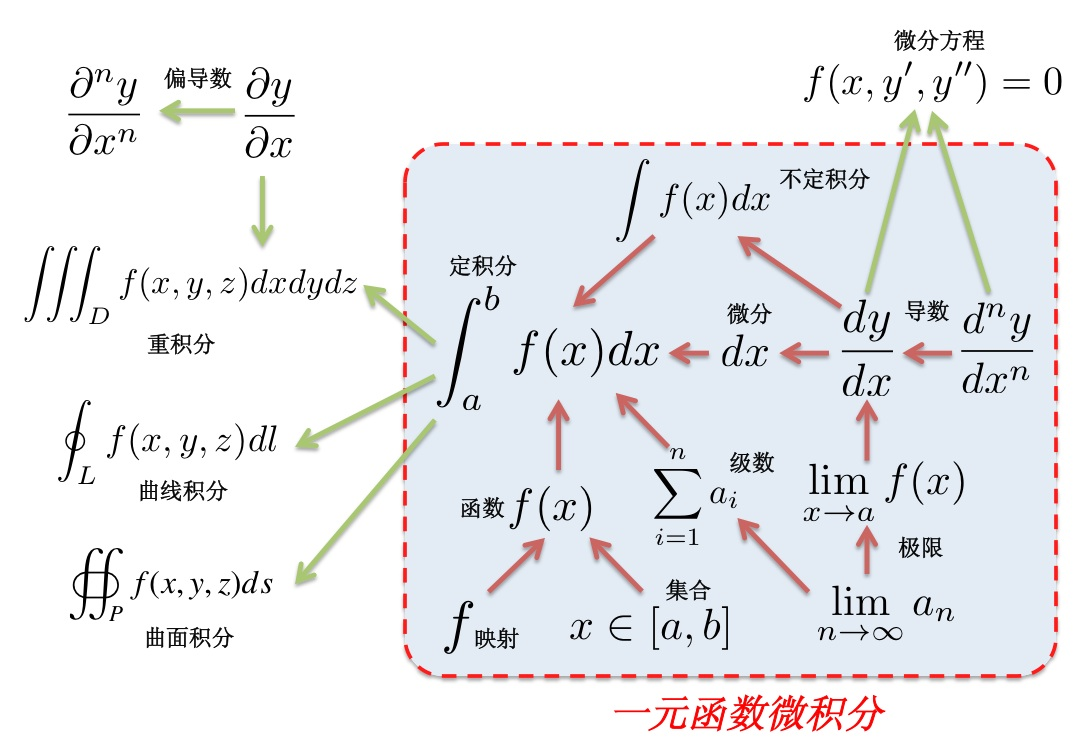
\includegraphics{./images/ch1/AM_architecture.jpg}}
% 	\caption{微积分中的主要概念及其关系\;
% 	({\it 个人整理,仅供参考})}
% % 	\label{图:0.1}
% \end{figure}

% \begin{center}
% 	\scalebox{0.3}{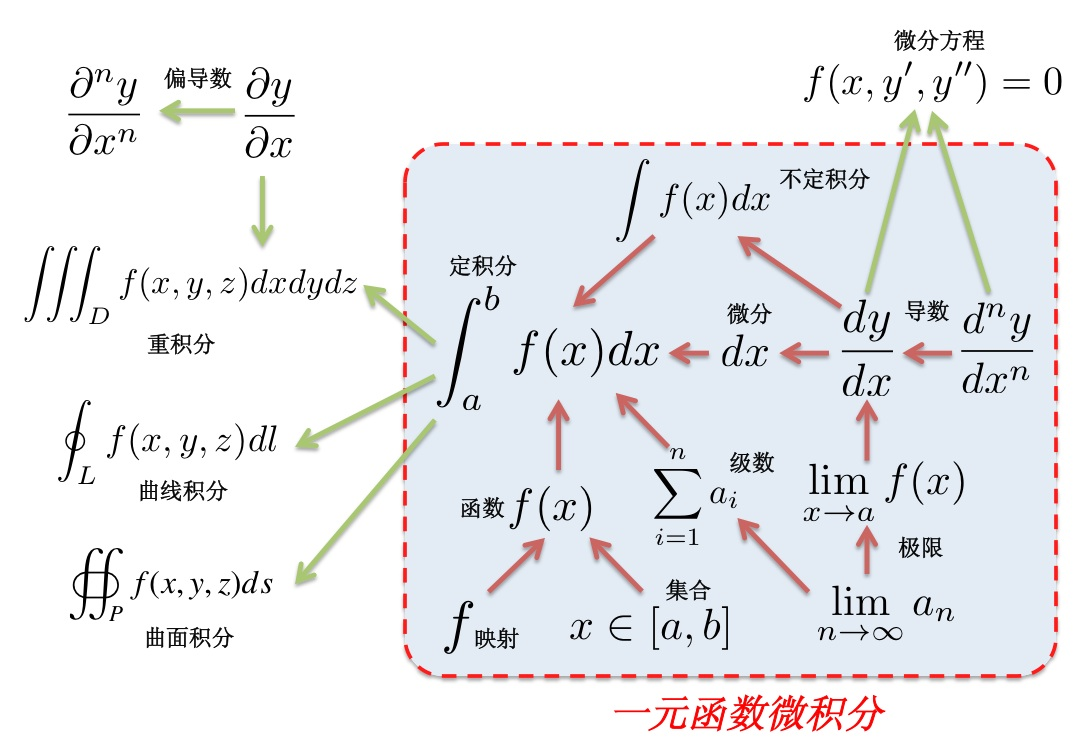
\includegraphics{./images/ch1/AM_architecture.jpg}}
% % 	\ps{上课前画好}
% \end{center}

\begin{center}
	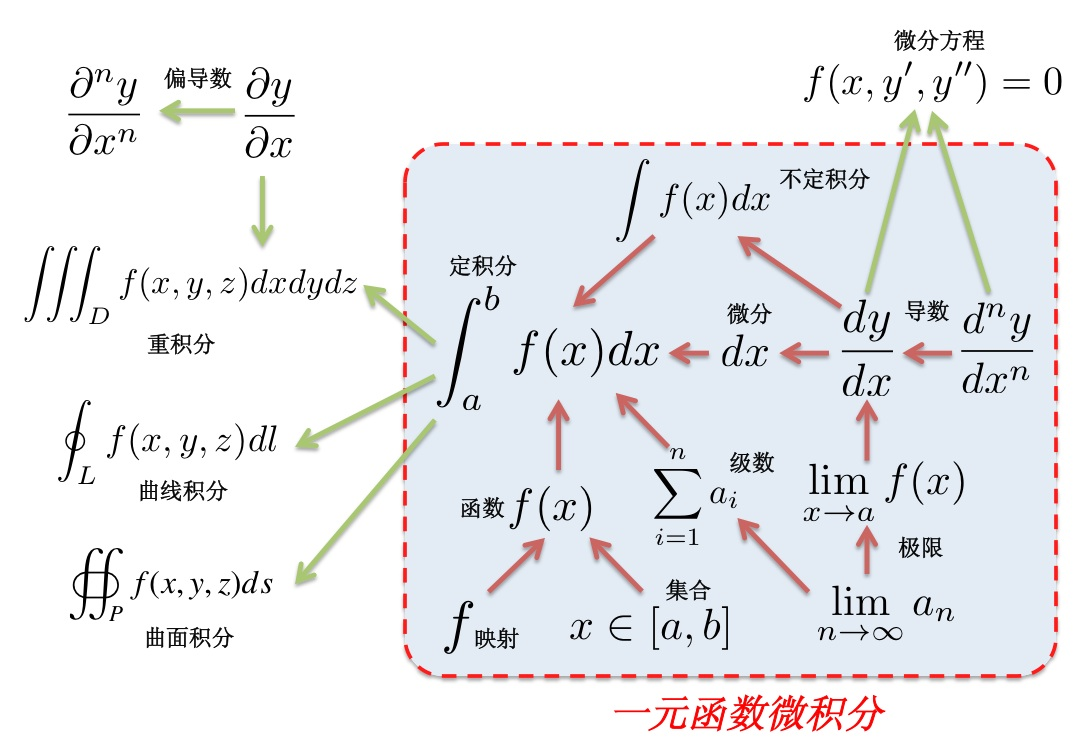
\includegraphics[width=0.8\textwidth]{./images/ch1/AM_architecture.jpg}
	
	{微积分中的主要概念及其关系\;
	({\it 个人整理,仅供参考})}
\end{center}

\begin{itemize}
	  \item {\bf Wikipedia——微积分(Calculus)} 
	\begin{itemize}
	  \item Latin: {\it a small stone used for counting}  
	  \item {\it a branch of mathematics focused on \underline{limits, functions,
	  	derivatives, integrals, and infinite series}} 
  	  \item {\it widespread application in \underline{science, economics,} 
  	  and \underline{engineering}} 
	  \item {\it constitues a major part of modern mathematics}
	  \item {\it 微}的意思是很小的东西,如微生物,{\it 积}就是加起来的意思,
	  {\it 积分}的意思就是把极小的东西加起来。微,是积的相反。 
	\end{itemize}
	\item {\bf John von Neumann} ({\small\it The Mathematician, 1947})
	\begin{itemize}
	  \item {\it The calculus was the \underline{first achievement} of modern
	  mathematics, and it is difficult to overestimate its importance.}
	\end{itemize} 
\end{itemize}

\subsection{为什么学}

微积分为什么如此重要,毫无疑问,与其在众多领域的应用密不可分,甚至可以说,
在其中绝大多数的问题中,微积分的作用是无可替代的。任何一门工科类的专业课程,
只要涉及与连续运动(变化)相关的问题,都不可避免地会以微积分作为其预备知识,
或者说,将这些课程视为微积分的应用也不为过。

当然,微积分不总是“美丽”的,因为它的美可能不是那么显而易见。我们很难用一两句话
来描述,微积分到底有什么用?它美在哪里?但是,一旦你理解了微积分背后的深刻思想,
开始能够将其应用于解决一些实际问题,或者通过它理解一些最前沿的科技成就时,
你一定会对它的美产生深深地赞叹,也许那时,再回头来看微积分的重要性也就不言而喻了。

学习微积分的过程也许会有些枯燥甚至痛苦\ps{“从前有棵树,叫高数,上面挂了很多人”}
,但它无疑是值得的,能够从看似单调痛苦的过程中领略数学的美丽,发现它的深刻与强大,
也是它作为“{\it 大学第一课}”\ps{无论从体量、难度还是学习的先后来看}所期望带给
大家的体验。

\begin{shaded}
	{\bf 知乎:学数学有什么好处?我们为什么要学数学?}
	\begin{itemize}
	  \item Engles:{\it 数学是一门研究现实世界的数量关系和空间形式的科学。}数学具有:
	  抽象性、精确性和应用的广泛性
	  \item Marx:{\it 一种科学只有在成功运用数学时,才算达到了真正完善的地步。}
	  \item Galileo:{\it “数学符号就是上帝用来书写自然这一伟大著作的统一语言,
	  不了解这些文字就不可能懂得自然的统一语言,只有用数学概念和公式所表达的物理世界
	  的性质才可认识……”}
	  \item Gauss:{数学是科学的女王}
	  \item 韩寒:{\it
	  我们生活中用到的数学估计到小学三年级就已经够用了。}然而在之后我们多年来学习的数学,
	  实际上塑造了我们一种理性的、条理的、系统化的思维方式。这种思维方式在我们解决自己
	  一生中遇到的诸多问题时,都有非常重要的作用。比如慎密的思考、分类的思想、排序的思想等。
	  很多东西其实都带有学习数学这个过程产生的影响,只是由于其作用方式非常隐晦,
	  也不容易被追溯其源头,我们平时不容易注意到罢了。
	  \item 王小波:{\it 我上大学时,有一次我的数学教授在课堂上讲到:我现在所教的数学,
	  你们也许一声都用不到,但我还要教,因为这些知识是好的,应该让你们知道。”}
	  \item 崔钢:{\it\b 1,用通用简洁的方式来表达自然规律。2,提供一些问题的分析手段。
	  3,提供认识世界的一种模式。4,了解自己的智力水平。.}
	\end{itemize}
	{\bf 豆瓣:为什么没人喜欢学习高等数学?木遥}
	\begin{itemize}
% 	  \item {\it 我完全不能理解,一个非数学或物理专业的学生怎么可能从这样的教育中获得一丝一毫的教益?
% 	  他怎么可能不发自内心地痛恨这门课程,然后在考完试之后的一个小时之内把所有内容忘得精光?
% 	  象三角代换这类积分技巧,不要说一个普通的心理学或者经济学专业的学生一辈子都用不到,
% 	  就连我也一辈子都用不到。就算在极其罕见的情形下需要求解这类问题,也完全可以求助于
% 	  wolframalpha.com 或者类似的工具。
	  \item 在我看来,在二十一世纪还要求一个普通学生手算积分,
	  就像是要求一个汽车驾校学员一定要从骑马学起一样。
	  \item \ldots 一本基于数学家思维方式写出来的教材,亦即在每一个课题上从最基本的定义
	  和定理开始堆砌,直到超出教材所可能涵盖的水平为止
	  \item 如果是我来编写大学数学教材,我会争取让每一个在大学里读过数学课的人都能回答这样的问题:
	  为什么人们能精确预测几十年后的日食,却没法精确预测明天的天气;为什么人们可以通过 https 
	  安全地浏览网页而不会被监听;为什么全球变暖的速度超过一个界限就变得不可逆了;
	  为什么把文本文件压缩成 zip 体积会减少很多,而 mp3 文件压缩成 zip 大小却几乎不变;
	  民生统计指标到底应该采用平均数还是中位数;当人们说两种乐器声音的音高相同而音色不同的时候
	  到底是什么意思\ldots\ldots这不是什么「趣味数学」,这就是数学。基础、重要、深刻、美的数学。
	  \item 在我的设想里,这才是大学基础数学教育所应该达成的任务。
	  {\it 不是培养一个非数学专业的现代人在数学领域的专业素质(这是无论如何也不可能成功的),
	  而是让一个人能够在非专业的前提下最大程度地掌握真正有用的现代数学知识,
	  了解数学家们的工作怎样在各个层面上和社会产生互动,以及社会在这个领域的投资得到了怎样的回报。}
	  别的科学门类的基础教育也应当是这样。
	\end{itemize}
	{\bf 知乎:学习编程及做程序员对微积分的要求高吗?}
\end{shaded}

\begin{itemize}
  \item {\bf 数学的三大功能}
  \begin{enumerate}
    \item 为学习其他知识(课程)提供数学工具
    \item 培养理性思维
    \item 弘扬数学文化
  \end{enumerate}
  \item {\bf 数学素质}
  \begin{enumerate}
    \item 从实际问题抽象出数学模型的能力
    \item 计算与分析的能力
    \item 了解和使用现代数学语言和符号的能力
    \item 使用数学软件学习和应用数学的能力
  \end{enumerate}
\end{itemize}

\subsection{怎么学}

\begin{itemize}
	\item {\bf 参考资料}
  	\begin{enumerate}
		\item {\bf 课程配套辅导}
	  	\begin{itemize}
	  	  \item \underline{同济大学数学系,高等数学(第七版,上、下),高等教育出版社,2014,北京}
	  	  	\ps{简称:\b 同济}  
	  	  \item 朱健民 等,高等数学(第二版,上、下),高等教育出版社,2015,北京
	  	  	\ps{简称:\b KD教材} 
	      \item 李建平 等,高等数学典型例题与解法(上、下),国防科技大学出版社,2009,长沙
	    	\ps{简称:\b 辅导书} 
	  	\end{itemize}
  		\item {\bf 参考书} 
  		\begin{itemize}
	    	\item 菲赫金哥尔茨,微积分学教程(第一至三卷),第8版,高等教育出版社,2006,北京
	    	  \dotfill{\it\b 读不懂不必勉强,它回答不了的微积分问题大学阶段你肯定碰不到} 
	    	\item James Stewart, Calculus(11th eds.)(影印版,上、下册),高等教育出版社,2016,北京
	    	  \dotfill{\it\b 大部头,但绝对浅显易懂}
	    	\item 斯蒂芬.弗莱彻.休森,数学桥,上海科技出版社,2010,上海
	    	  \ldots\dotfill{\it\b 值得常常拿出来读的数学书,一遍绝对不够} 
	    	\item William Dunham,微积分的历程——从牛顿到勒贝格,人民邮电出版社,2011,北京
	    	\dotfill{\it\b 了解微积分的历史,能够更好地理解其中深刻的思想} 
  		\end{itemize}
  		\item {\bf 在线资源}
  		\begin{itemize}
  		  \item 朱健民,高等数学(一-五),中国大学MOOC%,http://www.icourse163.org/course/NUDT-9004
  		    \ps{简称:\b MOOC}\ldots
  		    \dotfill{\it\b 缺课或者课上没听懂,就用它补补课}
  		  \item 李建平\,等,高等数学典型例题与解法(一、二),中国大学MOOC%,\\
  		    %http://www.icourse163.org/course/NUDT-1001979006
  		    \ldots\dotfill{\kaishu\b 辅导书的配套MOOC}
  		  \item 闫浩,高等数学习题课,学堂在线%,\\
  		     %https://xuetangx.com/courses/course-v1:BUPT+3412113011+2017_T2/about
  		     \dotfill{\it\b 讲得棒极了,这老师其实是清华的}
%   		  \item 李建平\,等,微积分CAP,中国大学MOOC%,
  		     %http://www.icourse163.org/course/NUDT-1001626005
%   		    \dotfill{\it\b 高中没学好,来这补一补}
		\end{itemize} 
		\item {\bf 扩展阅读}\dotfill{\it\b 读一些课外书,让学习显得不那么枯燥}
		\begin{itemize}
		  \item 基斯.德夫林,数学思维导论,人民邮电出版社,2016,北京
		  \item G.波利亚,怎样解题:数学思维的新方法,上海科技教育出版社,2011,上海
		  \item 李学数,数学与数学家的故事(1-5),上海科学技术出版社,2015,上海
		  \item 塞德里克·维拉尼\,等,一个定理的诞生:我与菲尔茨奖的一千个日夜,人民邮电出版社,2016,北京
		  \item 春日真人,庞家莱猜想:追寻宇宙的形状,人民邮电出版社,2015,北京
		  \item 蒂莫西.高尔斯,数学,译林出版社,2014,南京
		  \item 吴军,数学之美,人民邮电出版社,2016,北京
		  \item 李建平,漫谈数学与军事,中国大学MOOC
		  \item \ldots\ldots
		\end{itemize}
	\end{enumerate}
	\item {\bf 学习方法}
% 	\begin{itemize}
% 	  		\item {\bf 听课}\dotfill {\bf 30}
% 		\begin{itemize}
% 	  		  \item 典型问题、典型方法
% 	    	  \item 师傅领进门,修行在个人
% 	 	\end{itemize}
% 	  		\item {\bf 练习}\dotfill {\bf 50}
% 	 	\begin{itemize}
% 	    		\item 熟能生巧!
% 	    		\item 记忆!琢磨!
% 	  	\end{itemize}
% 	  		\item {\bf 思考}\dotfill {\bf 20}
% 	  	\begin{itemize}
% 	    		\item 总结!
% 	    		\item 质疑!
% 	  	\end{itemize}
% 	\end{itemize}
	\begin{enumerate}
	  \item {\bf 预习:}课前3-5分钟,快速翻阅教材,浏览本讲内容梗概,
	  标记出新的名词和例题,试着理解其大概意思,确保听课时心中有数;
	  \item {\bf 听课:}抓住关键思路,卡住了或者有疑点立即举手问,
	  简要记笔记\ps{推荐:\b 康奈尔笔记法},重点记思路和书本上没有的内容
	  \item {\bf 复习:}要么读教材,要么读笔记,也可以先作习题,搞不定
	  再回来翻书查笔记,重在理清思路\ps{重要概念,典型问题,典型方法},
	  消化细节,肯花时间才有好的效果
	  \item {\bf 练习:}作业之外,有选择地作题,学习也是个熟能生巧的过程,
	  提高效率是关键\\
	  G.Polya:{\it 我们的任何一门学问都由知识和技能组成。如果你对初等或高等数学的研究工作
	  的确有真正的经验的话,那么你对下述这一点将毫不怀疑:在数学中,技能比仅仅掌握
	  一些知识要重要得多。什么是技能呢?数学技能就是解题能力——不仅能解决一般的问题,
	  而且能解决需要某种程度的独立思考、判断力、独创性和想象力的问题}
	  \item {\bf 思考:}多琢磨,让知识点在大脑中结成网络,融会贯通,
	  会提问是思考能力的体现\ps{Einstein:提出一个问题往往比解决一个问题更重要!}
	  \centerline{\it What$\to$How$\to$Why$\to$Why not$\to$What if}
	\end{enumerate}
\end{itemize}

\section{几点要求}
\begin{itemize}
	\item {\bf 课堂:安静!安静!!安静!!!}
	尊重他人学习的权利,安排好自己的时间
	
	{\bf - No to}
	  \begin{itemize}
	    \item Chatting
	    \item zZZ\ldots
	    \item anything noisy
	    \item \ldots
	  \end{itemize}
	{\bf - Yes to}
  \begin{itemize}
    \item listen to me
    \item discuss {\bf with me}
    \item do sth. you like {\bf quietly}
    \item zzz\ldots
    \item leave/enter the classroom {\bf quietly}
    \item \ldots
  \end{itemize}
  \item {\bf 作业}
  \begin{center}
  	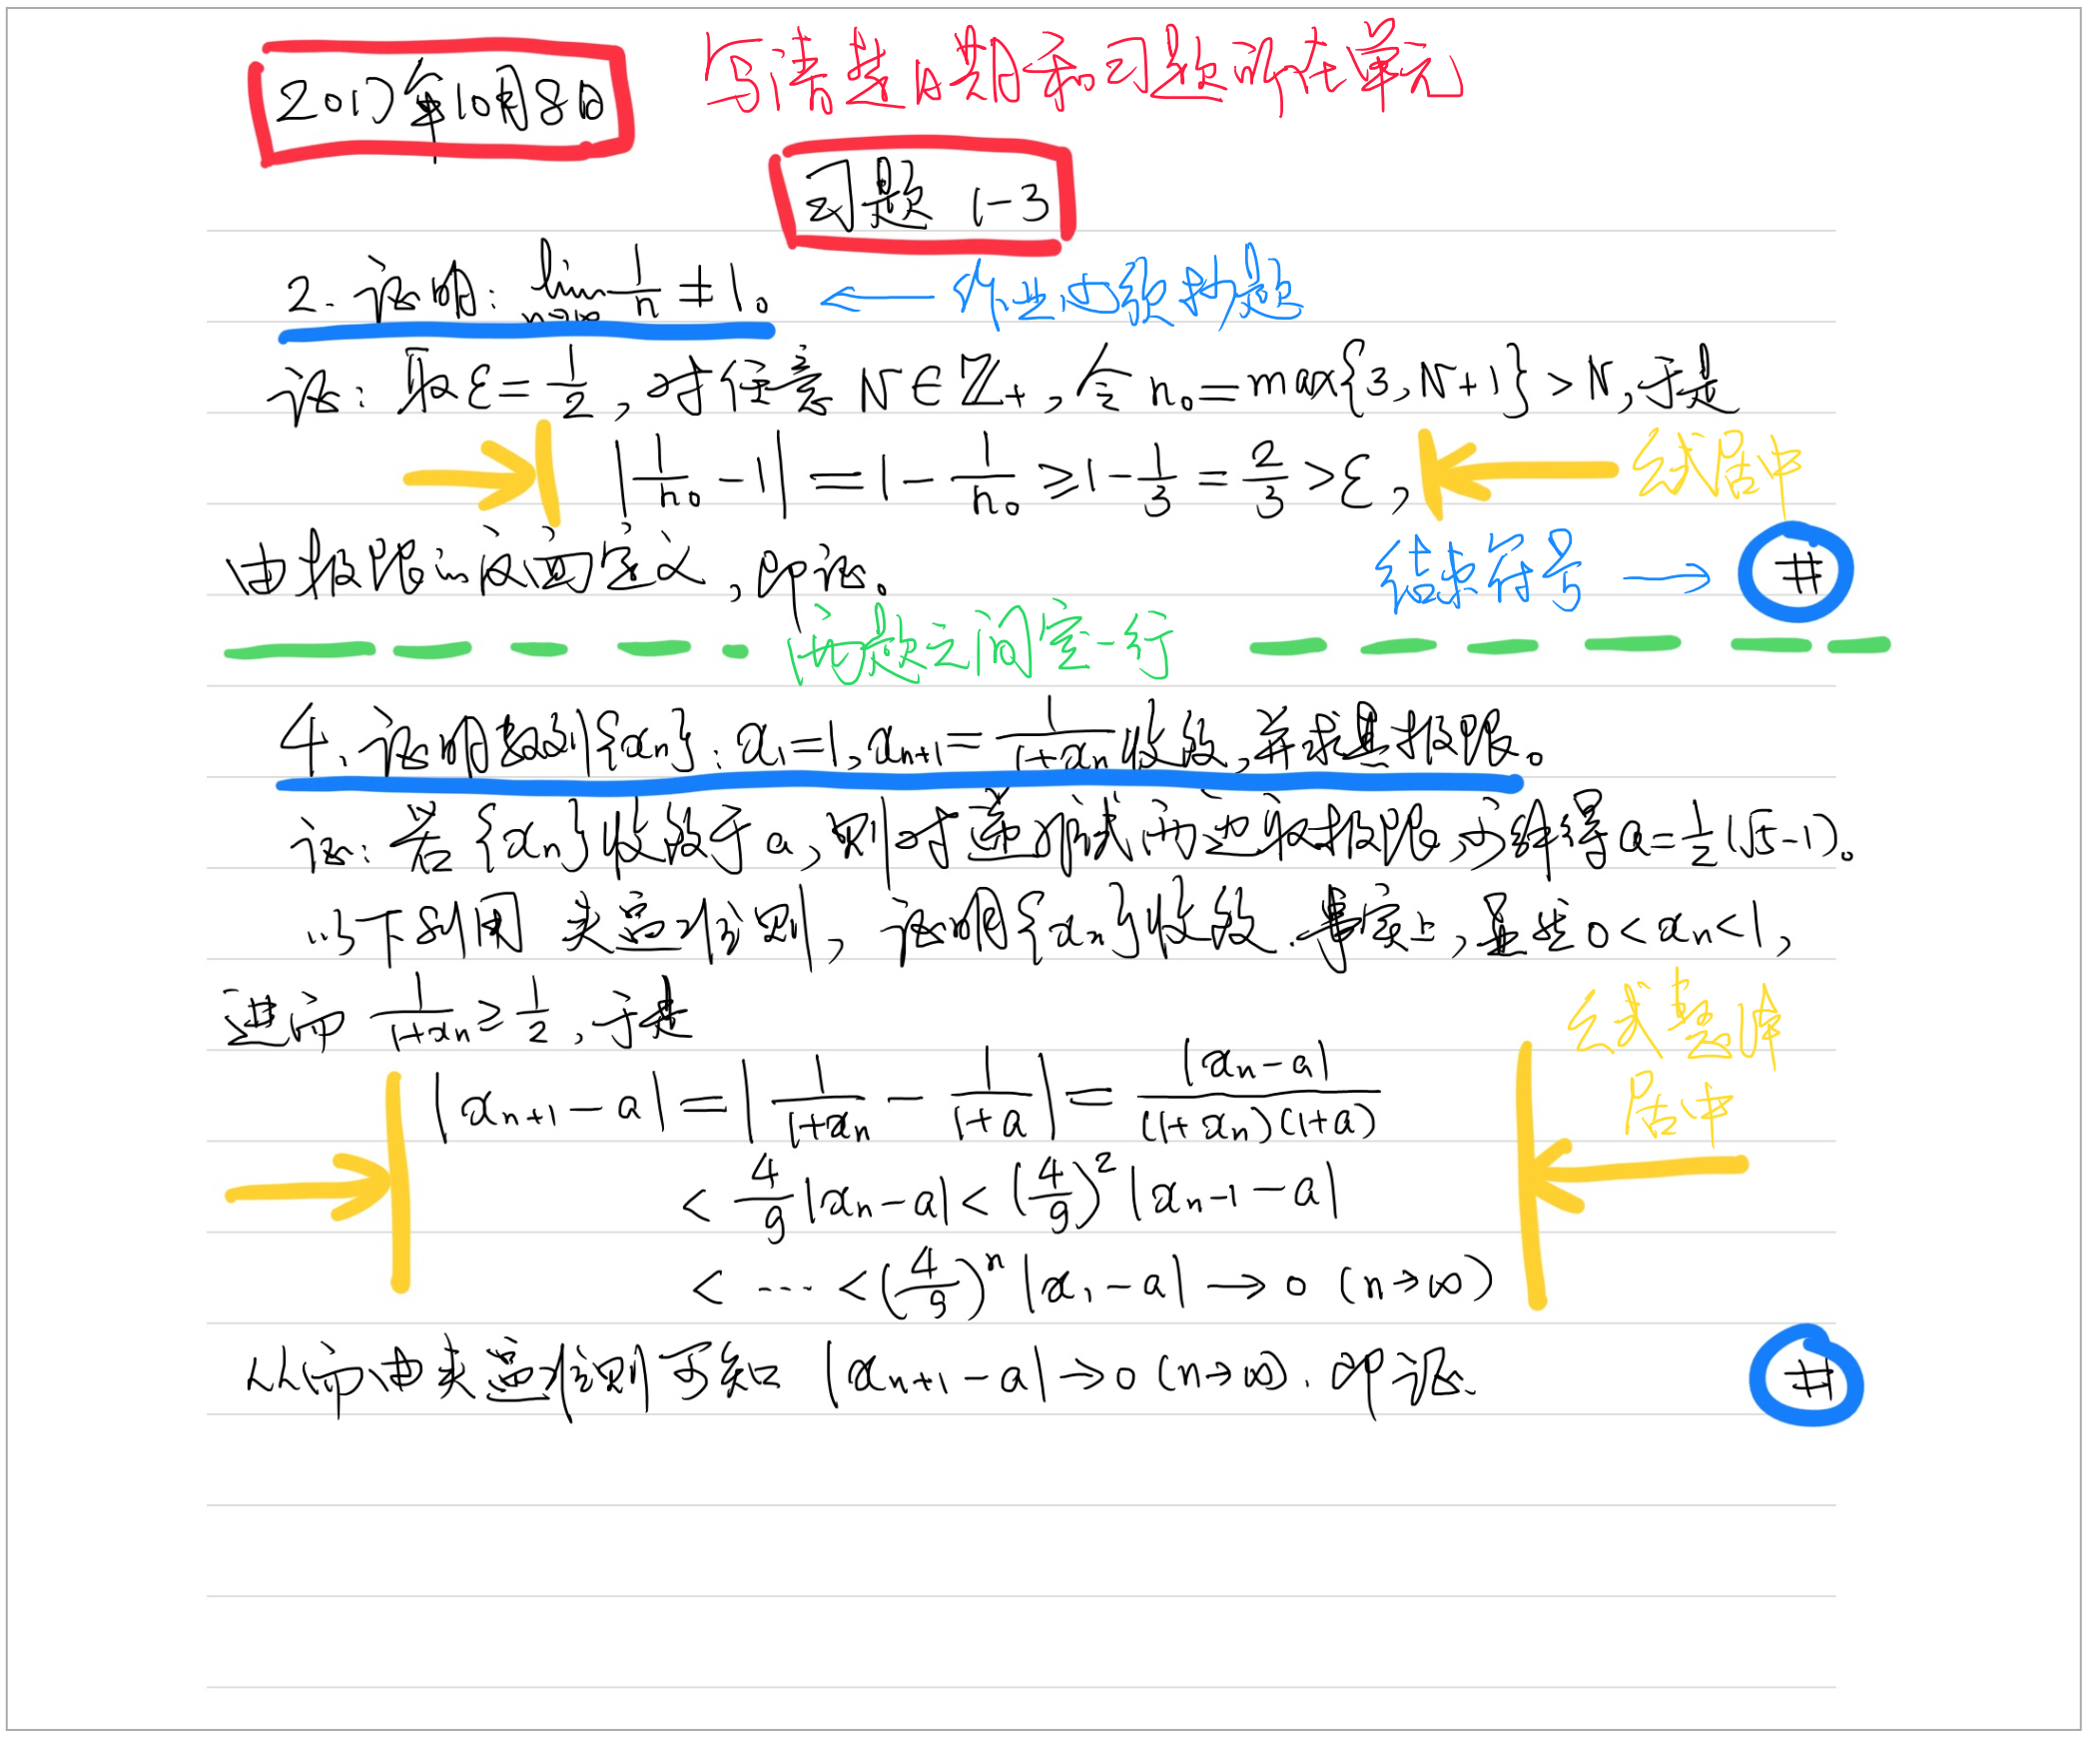
\includegraphics[width=0.95\textwidth]{./images/00/hw-sample.jpg}
  	
  	作业书写参考样式({\it 以黑色字体为准,彩色部分为格式说明})
  \end{center}
  \begin{itemize}
    \item 作业书写的规范
    \begin{enumerate}
      \item 写清楚作业日期(对应讲课的日期)和习题所在单元;
      \item 作业必须抄题,写清楚题号
	  \item 解题过程以“证:”或“解:”开始,以$\#$号结束;
	  \item 公式整体居中书写;
	  \item 无论大题小题,两题之间空一行;
	  \item 不允许使用铅笔、红笔书写作业,可以用铅笔画图;
	  \item 作业本不许分栏使用;
	  \item 文字、符号书写清晰规范,尽量少涂改。
    \end{enumerate}    
    \item no copy ??!
    \item 及时订正错误,补上缺漏
  \end{itemize}
	\item {\bf 答疑}
	  \begin{itemize}
	    \item 每周一次面对面答疑,1-2小时
	    \item 提问题的能力不完全是天生的,脸皮要厚一点
	    \item 综合利用各种手段(微信、网站、邮件、\ldots)
	  \end{itemize}
% 	  \item {\bf 从善如流}
\end{itemize}

\section{关于考试}

以下是2017-2018学年开始实施的“{\it 新政}”:

考试分为{\it 形成性考试}和{\it 终结性考试}两个部分,两部分成绩按照$40\%$和$60\%$的比例综合
得到最终的课程期末成绩。

每学期末设一次终结性考试,采用闭卷笔试形式。{\color{red}\bf 终结性考试不及格,
则课程成绩不合格!}

每学期的形成性考试分为四个部分,一是{\it 平时作业和表现}成绩,占$10\%$,剩下的为三次
{\it 单元测试}成绩,各占$10\%$。

单元测验的形式为笔试或网络测试,具体待定。

\newpage

\begin{shaded}
	{\bf\Large Cornell Note-Taking System}\hfill{\it 康奈尔笔记法(5R笔记法)}
	
	\bigskip
	
	这一方法适用于一切依赖讲授或自学的学习过程,特别是对于听课笔记,5R笔记法堪称首选。
	该方法的重点是记与学、思考与运用的结合,以及将笔记的记录与完善作为学习的过程载体。
	最终完成的笔记类似于下图:
	
% 	\begin{figure}[htbp]
% 		\centering
% 		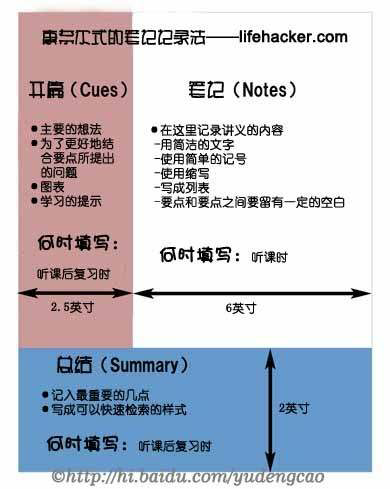
\includegraphics[width=0.4\textwidth]{./images/00/Cornell-NTS/NTS-CH.jpg}\quad
%  		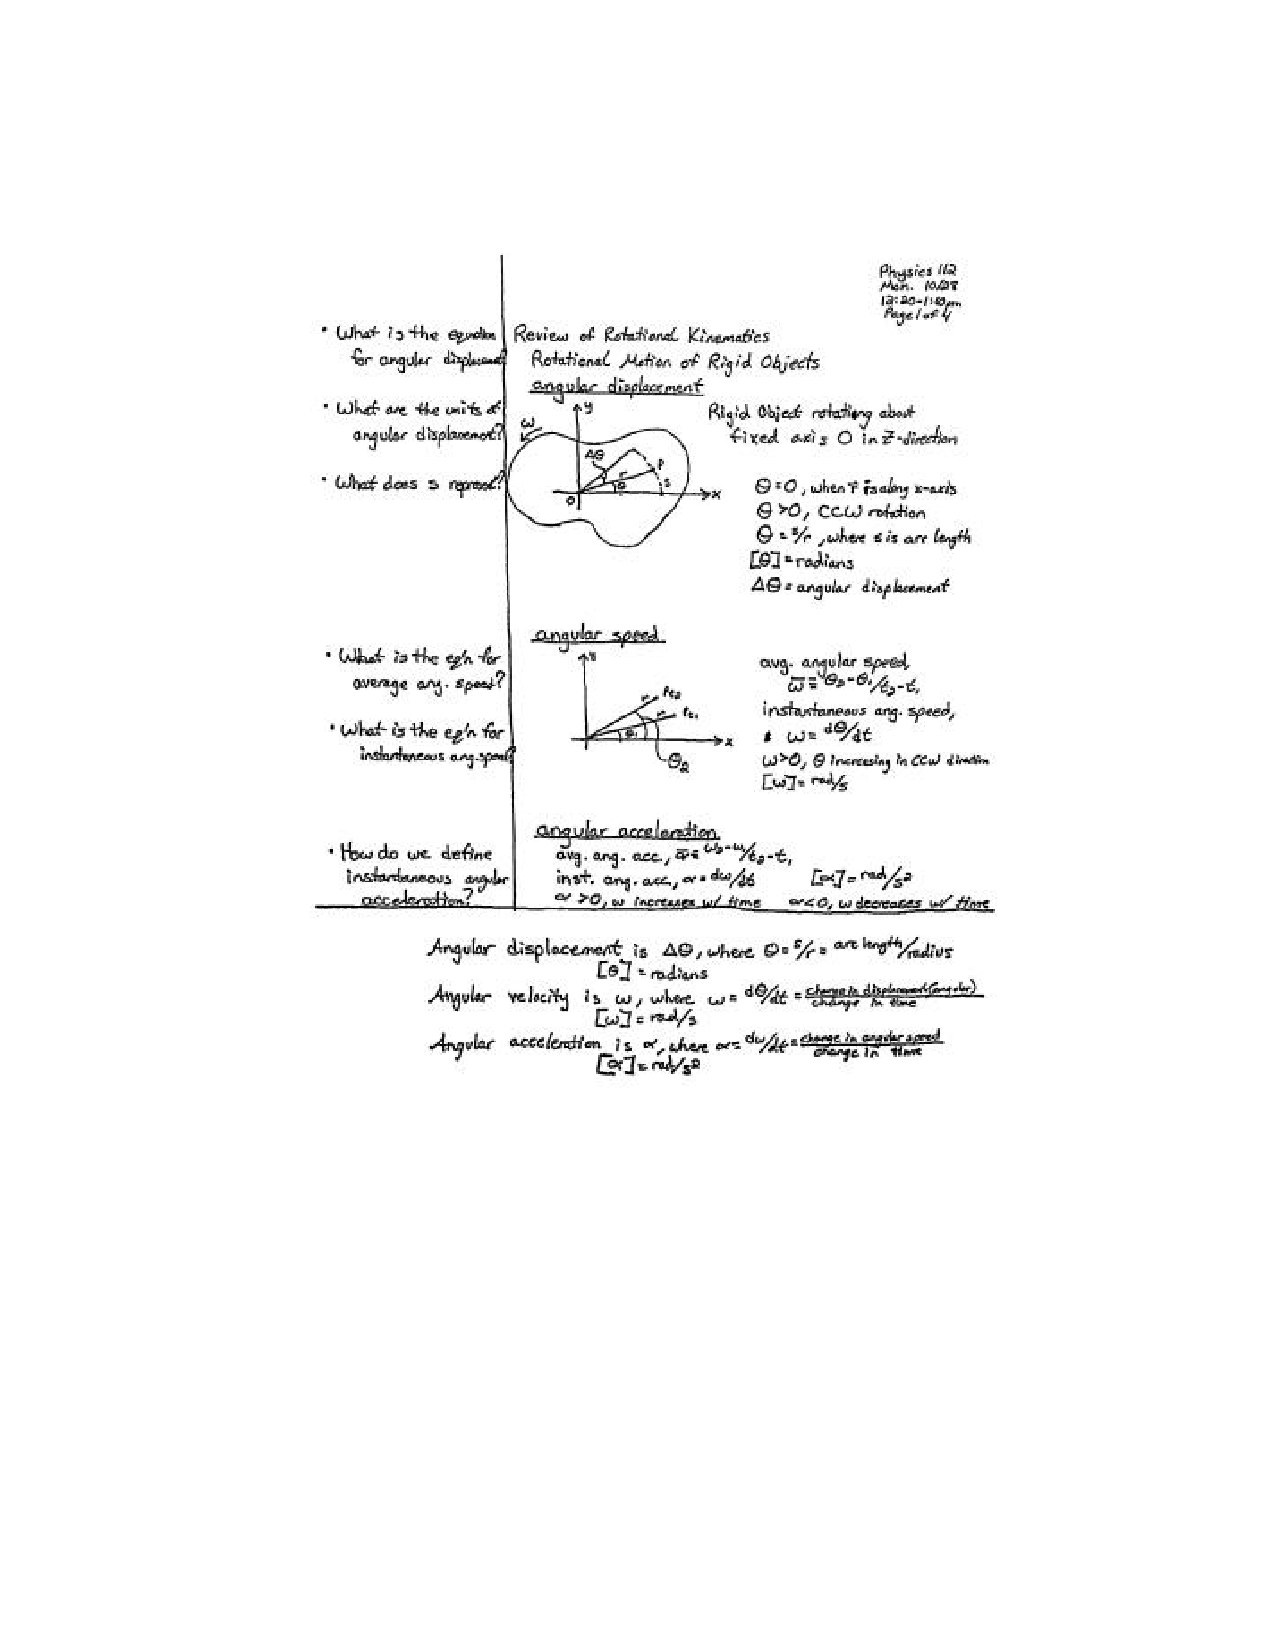
\includegraphics[height=8cm]{./images/00/Cornell-NTS/exCNTS.pdf}
% 	\end{figure}
	
	\begin{center}
		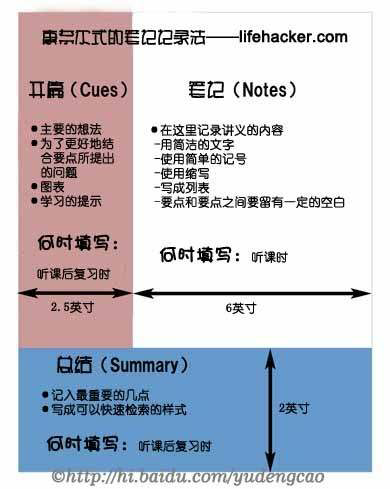
\includegraphics[height=8cm]{./images/00/Cornell-NTS/NTS-CH.jpg}\quad
		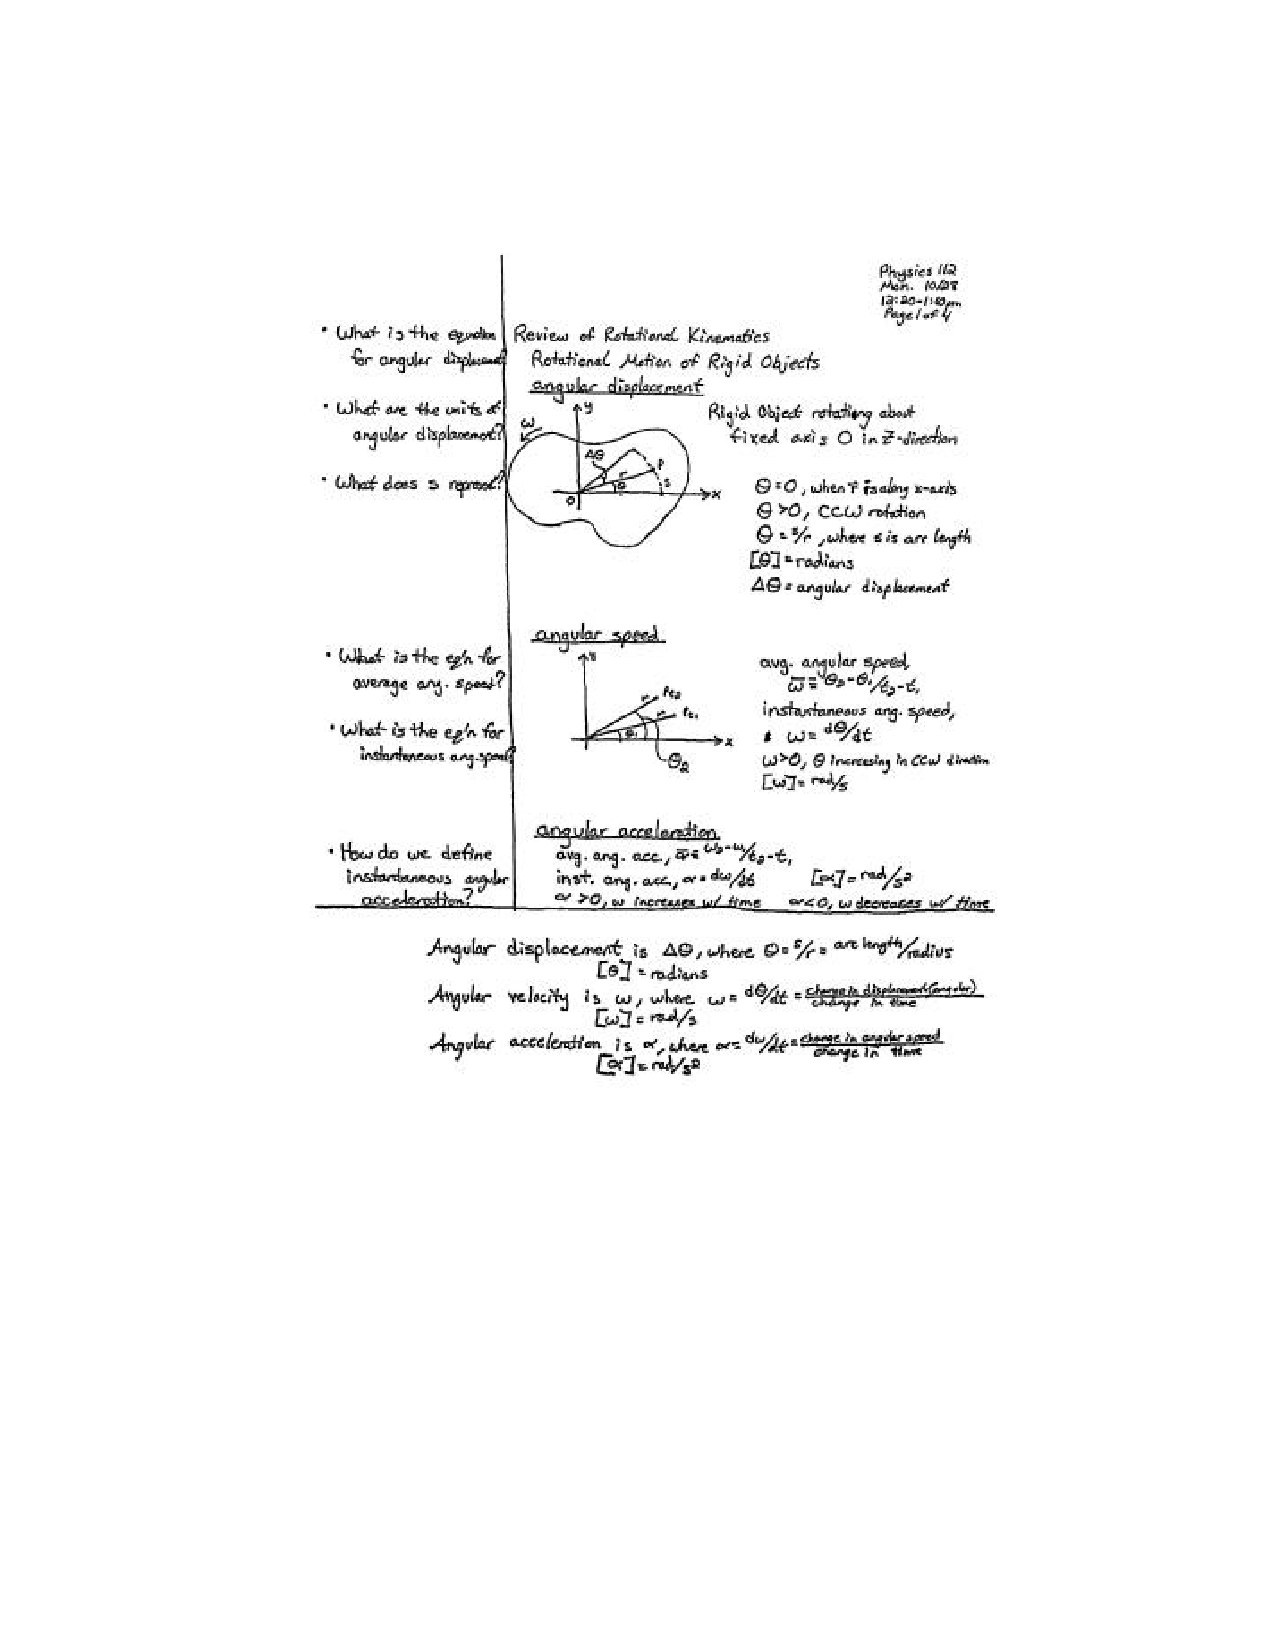
\includegraphics[height=8cm]{./images/00/Cornell-NTS/exCNTS.pdf}
	\end{center}
	
	笔记的行程过程可以分为所谓的{\bf 5R}:
	
	\begin{enumerate}[Step1]
	  \setlength{\itemindent}{1cm}
	  \item {\it 记录(Record):}在听讲或阅读过程中,
	  在主栏(将笔记本的一页分为左大右小两部分,
	  左侧为主栏,右侧为副栏)内尽量多记有意义的论据、概念等讲课内容。
	  \item {\it 简化(Reduce):}下课以后,尽可能及早将这些论据、概念简明扼要地概括(简化)
	  在回忆栏,即副栏。
	  \item {\it 背诵(Recite):}把主栏遮住,只用回忆栏中的摘记提示,
	  尽量完满地叙述课堂上讲过的内容。
	  \item {\it 思考(Reflect):}将自己的听课随感、意见、经验体会之类的内容,
	  与讲课内容区分开,写在卡片或笔记本的某一单独部分,加上标题和索引,
	  编制成提纲、摘要,分成类目。并随时归档。
	  \item {\it 复习(Review):}每周花十分钟左右时间,快速复习笔记,主要是先看回忆栏,
	  适当看主栏。
	\end{enumerate}
	
	在课本、参考书原文的旁边加上各种符号(如直线、双线、黑点、圆圈、
	曲线、箭头、红线、蓝线、三角、方框、着重号、惊叹号、问号等等),便于找出重点,
	加深印象,或提出质疑。什么符号代表什么意思,自己掌握即可,但最好形成一套比较
	稳定的符号系统。这种方法特别适合于自学笔记和预习笔记。
	
	操作时注意以下一些准则:
	{\it 读完后再做记号,要非常善于选择,用自己的话进行注记,形式和过程力求简洁,迅速,整齐}
	
	笔记的加工:{\it 忆$\to$补$\to$改$\to$编$\to$分$\to$舍$\to$记}	
\end{shaded}

\chapter{函数与极限}

极限是微积分理论中最基础的概念(定义和讨论微分和积分的基础),理解极限的数学
定义与性质,掌握极限收敛判定和极限计算的方法,是真正深入理解微积分的第一步。

极限的数学定义(更具体地称为“$\e-\delta$”或“$\e-N$”定义)是进入微积分学习
后可能遇到的第一个难点(难度可能因人而异),因为它兼具形式的抽象性和逻辑的复杂性
(因为必须严谨、准确)。学会用数学和逻辑的语言表达某个概念、性质和进行推理、分析,
也是通过微积分的学习需要锻炼和培养的能力。从这个角度来说,极限概念的重要性就更加
不言而喻了。

% {\bf 关键词:}集合、集合论、映射、函数、曲线及其表示

% \setcounter{section}{-1}

\section{集合、映射与函数}

\subsubsection{集合}

{\it Cantor,1874:}\ps{对于集合,“我们只需描述它,而不必给出精确的定义”}
所谓{\it 集合},是指把一些个体({\it 元素}) 放在一起考虑时它们形成的整体。
\begin{itemize}
  \setlength{\itemindent}{1cm}
  \item 关系符号:$\subset, \in, =, \subseteq, \neq$
  \item 运算符号:$\cap,\cup, \setminus, \bar{A}, \times, +, - $\quad ({\it
  依次为:交、并、差、补、笛卡尔积、不交并、差})
\end{itemize}
	
本门课程中常见(用)的集合:
$$\b\mathbb{N}\subset\mathbb{Z}\subset\mathbb{Q}
\subset\mathbb{R}\subset\mathbb{C}$$
\quad({\it 依次为:自然数集\ps{\b 国内教材一般约定,自然数集包含数$0$}、
整数集\ps{德语Zahlen(数)的首字母}、有理数集、无理数集和复数集})


通过集合的{\it 笛卡尔积}“$\times$” 可以定义更{\it
“高维”}的集合,例如:$\mathbb{R}$表示数轴(上的所有点构成的集合),则
$${\b \mathbb{R}^2=\mathbb{R}\times\mathbb{R}}$$
表示全平面(上的所有点构成的集合)

{\bf 【区间和邻域】}

{\bf 例:}给定$a,b\in\mathbb{R},a<b$,区间$(a,b)=\{x\in\mathbb{R}|a<x<b\}$

{\bf 例:}记实数集$\mathbb{R}=(-\infty,+\infty)$

{\bf 注意:}{\b 由于$\pm\infty$都不是具体的数,因此在本门课程中,除非特别说明,形如
\ps{\b 请对讲义中蓝色字体的部分多加留意!}
$$x=+\infty\quad\mbox{或}\quad x=-\infty$$
的写法总是错误的,而只能写
$$x\to+\infty\quad\mbox{或}\quad x\to\infty$$
}

{\bf 邻域}
$${\b U(a,\delta)}=(a-\delta,a+\delta)=\{x\in\mathbb{R}||x-a|<\delta\}$$
含义为:实数集中所有与$a$绝对值小于(距离小于)$\delta$的数(点)构成的集合

{\bf 例:}
$$(a,b)=U\left(\df{a+b}2,\df{b-a}2\right)$$

{\bf 去心邻域}
%\ps{同济写做$U^0(a,\delta)$,我们在使用是可不加区别}
$${\b
U_0(a,\delta)}=(a-\delta,a+\delta)-\{a\}=\{x\in\mathbb{R}|0<|x-a|<\delta\}$$

{\bf 无穷邻域}*\ps{名词后面加星号的,表示了解即可}
$$\{x\in\mathbb{R}||x|>M\},\;M>0$$

{\bf 问:}以上无穷邻域可以写成类似$U(\infty,M)$的形式吗?

答:因为$\infty$不是一个具体的数(点),
所以为了避免误解,我们不会这么写!

{\bf 半邻域,左(右)邻域},例如:点$a$的右半邻域为
$$\{x\in\mathbb{R}|a<x<a+\delta\}$$

\ps{灰色背景内容为扩展知识,了解即可}

\begin{shaded}

{\bf 集合论、Russell Paradox与公理系统}

	{\it Cantor,1874:}朴素集合论的诞生。	

	{\it Poincare,1900,国际数学家大会:} 
		 {“\ldots 借助集合论概念,我们可以建造整个数学大厦\ldots  今天,我们可以说绝对的严格性已经达到了\ldots”}
	
	{\it Russell, 1901:}只给不给自己理发的人理发的理发师该不该给自己理发?
	
	“由所有不包含集合自身的集合所构成的集合”,记为$S$。不论$S$是不是自身的元素,按照$S$的定义都会有矛盾。
	
	设$x\in A$表示:$A$给$x$理发, 定义
	$$A=\{x|x\notin x\},$$ 
	
	问:$A\in A$还是$A\notin A$? 
	
% 	\ba{罗素悖论导致了第三次“数学危机”的出现!}
	{{\bf {第三次“数学危机”}}(Frege,1901,《算术基础》)}
		“在工作结束之后发现那大厦的基础已经动摇,对于一个科学工作者来说,没有比这更不幸的了”
		
	\begin{itemize}
	  \item {{\bf 无限抽象原则}(Cantor,Frege):} 任意给定某个条件就可以确定一个集合。(每个概念的外延可以确定一个集合)
	  \item {\bf 观点:}不加限制地使用无限抽象原则将导致罗素悖论
	  \item {{\bf 有限抽象原则}(限制公理):} 如果已知一个集合和一个给定的条件,
	  则该集合中所有满足条件的元素{\it 可以}构成一个集合。
	  \item {\bf ZF(Zermelo-Fraenkel)公理化集合论}
	  (Zermelo-Fraenkel Set Theory):包含选择公理的称ZFC,否则为ZF。
	  
	  {\bf 命题:}在ZF/ZFC中,无法定义包含所有集合的集合。
	
	[证]:反证法。设$A$是一个这样的集合。定义
	$$B=\{x\in A|x\notin x\}$$
	若
	$B\in A$,则必有$B\in B$或$B\notin B$。而若$B\in B$,可推出$B\notin B$;同理,
	由$B\notin B$,也可推出$B\in B$。从而$B\notin A$,推出矛盾。这说明$B$的定义存在问题,故知假设错误。

	\item {\bf 公理(Axiom):}无须证明即为正确的命题。
	\begin{itemize}
	  \item {\it Engles:}数学上的所谓公理,是数学需要用作自己出发点的少数思想上的规定 
	  \item {\bf ZFS系统:}公理就是一些关于逻辑符号{“$\in$”}和{字母}的组合使用方法的约定
	  \item {\bf 公理化方法}是构建现代数学理论体系的基石
	\end{itemize}
	\item {\bf {数学等于永恒的真理吗?}}
	\end{itemize}
	
	{\bf 注:}ZFC有无穷多个公理,因为替代公理实际上是公理模式。已知ZFC和ZF集合论
	二者都不能用有限数目个公理来完全公式化。
	
	{\bf 讨论:}公理(Axiom)、定理(Theorem)、定律(Law)、假设(Assumption)、
	引理(Lemma)、推论(Corallary)、猜想(Conjuction)有何异同?
	{\b\dotfill\it 建议做常识性了解!}
	
	{\it 试答:这些概念都是对自然规律或数学规则的表达。
	
	公理是数学及其相近领域所使用的概念,即在数学理论体系中无须证明即视为正确的命题(例如:
	两点之间直线最短),是数学理论体系的出发点。通过推理和演绎,我们可以在公理的基础上
	进一步推出新的结论,这些结论我们通常称为定理,引理和推论则是定理推导的中间和后续结果。
	使用不同的公理作为出发点,可能得到完全不同的理论体系,例如:非欧几何的多条基本公设(公理
	的另一种说法)就是和欧式几何不同的,这导致二者的理论体系看起来大相径庭。
	
	我们目前所使用的公理多数来源于生活中的直观体验,是一种对直觉观察的抽象描述。而由于
	我们对自然世界认识的局限性,这些描述本身可能是不精确甚至是不正确的。从这个意义上说,我们
	更应该说公理其实是我们对于客观规律的假定,是先验的,但也是可以有所调整和变化的。
	
	定律也具有类似的特点,因为人类总是在不断改进和加深对于自然世界的认识。定律更多
	地出现于物理、化学等非抽象领域,体现的是对自然规律的描述。定律背后通常存在一些的
	基本假定(例如:原子是不可分的、光既是例子又是波),定律的发现需要以重复实验为基础,
	定律的描述中一部分是可以用数学工具来刻画的(例如万有引力定律、质能方程)。
	
	公理、定理、定律的共性之处在于它们在各自的领域中或背景下,都被视为是“正确的”(请注意在数学中
	正确和可证明有时是被混同的),是被验证、证明或直接假定为真的命题,而猜想则是被
	猜测为真,但未经过这些过程,所以仍无法断言为真的。当今的数学界,仍有大量的猜想有待证明或证否,
	这些问题所代表的恰恰是数学的最前沿。
	}
\end{shaded}
	
{\bf 【实数集的性质】}
	\begin{enumerate} 
	  \item {\bf 有序性:}即任何两个实数均可以比大小\quad (注:$\mathbb{R}^2$、$\mathbb{C}$不具备有序性) 
	  \ps{$\mathbb{R}$是全序的,而$\mathbb{R}^2$、$\mathbb{C}$在一定的度量下
	  是半序的}
	  \item {\bf 完备性(连续性): }实数集与数轴上的点之间存在一一对应
	  \ps{这是KD教材上的说法,不够严谨!}
	  
	  {\bf{连续性公理(确界原理):}}非空有{上界}的实数集必有{上确界} (最小的上界)\\
	  {\bf 注}:实数集的完备性更准确的说法应该是:
	  {\it 实数集的任意非空有上界的子集都有上确界,且该上确界为实数}
	\end{enumerate}
	
	为了更好地理解确界原理,必须对集合的有界性以及上(下)界和上(下)确界的概念有非常准确的理解:
	
	{\bf 上界:}$M\in\mathbb{R}$称为集合$A\subset\mathbb{R}$的上界,是指:对任意$x\in A$,均有
	$x\leq M$。
	
	{\bf 集合$A$有上界:}存在$M\in\mathbb{R}$为$A$的上界\ps{\b 显然上界是不唯一的!}
	
	{\bf 集合$A$有界:}即$A$同时有上下界。
	
	设$M$和$m$分别为$A$的上界和下界,令$M^*=\max\{|m|,|M|\}$,则可以证明,对
	任意$x\in A$,有$-M^*\leq x\leq M^*$,或$|x|\leq M^*$。这个命题
	也常常作为集合有界的定义。
	
	{\bf 上确界:}{\b
	$M_0\in\mathbb{R}$称为集合$A\subset\mathbb{R}$的上确界
	(记为$M_0=\mathrm{sup}A$),
	是指:$M_0$是$A$的最小上界},也即同时有:
	\ps{准确理解上确界的概念是本章的难点!\\
	下确界记为:\b$\mathrm{inf}A$}
	\begin{enumerate}[(1)]
	  \setlength{\itemindent}{1cm}
	  \item $M_0$是$A$的上界,即:对任意$x\in A$,均有$x\leq M_0$;
	  \item $A$的任意上界都不小于$M_0$,即:若$M$为$A$的一个上界,则$M_0\leq M$。
	\end{enumerate}
	
	{\bf $M_0$为$A$的上确界}一个常见的数学定义为:{\b 对任意小的$\e>0$,
	都存在某个与之对应的$x_{\e}\in A$,使得$M_0-\e<x_{\e}\leq M_0$,}
	或者简写作
	$$\b M_0=\mathrm{sup}A\;\Leftrightarrow\;
	\forall\e>0,\;\exists x_{\e}\in A,\;M_0-\e<x_{\e}\leq M_0.$$
	
	{\bf 思考:}上面这个对上确界的数学定义
	\ps{大多数时候,我们并不严格区分{\b 数学定义}和{\b 概念},只是数学定义通常
	会用更抽象的数学符号和更严谨的逻辑语言来表达,今后我们所说的{\b 定义}即指
	数学定义或概念}
	,与前面我们讨论的上确界的概念之间	是什么关系?你能否证明它们是等价的?
	
	{\bf 思考:}上确界和最大值有什么异同?如何确定一个集合的上确界?
	
	{\bf 讨论:}{\b 有理数集不满足连续性公理!}准确地说就是:有理数集的非空有上界的子集,
	其上确界未必是有理数	(但肯定是实数)!为了说明这一点,来看下面的例子:
% 	\ps{如果将取上确界视为一种集合运算,这里所说的完备性可以理解为,
% 	该集合对于取上确界的运算封闭}
	
	{\bf 例:}考虑集合$A=\left\{\left(1+\frac 1n\right)^n|n\in\mathbb{N}\right\}$,因为
	有理数的有限次四则运算仍是有理数,故显然$A\subset\mathbb{Q}$。如下图所示,集合$A$中的点如果按照
	$n$从小到大的顺序排列,恰好是构成一个随$n$单调递增有上界($3$就是它的一个上界)的数列,也即:
	$$\left(1+\frac11\right)^1<\left(1+\frac12\right)^2<\left(1+\frac13\right)^3<\ldots
	\left(1+\frac1n\right)^n<\ldots<3,$$
	\begin{center}
		\resizebox{!}{6cm}{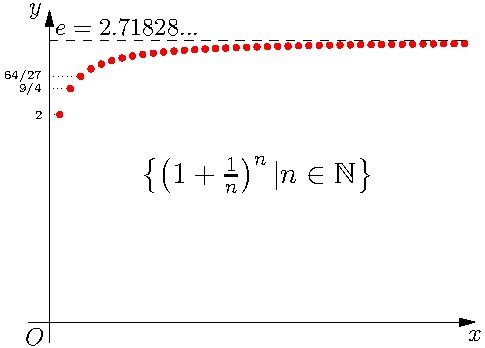
\includegraphics{./images/ch1/e-notin-N.pdf}}
% 		\resizebox{!}{4.8cm}{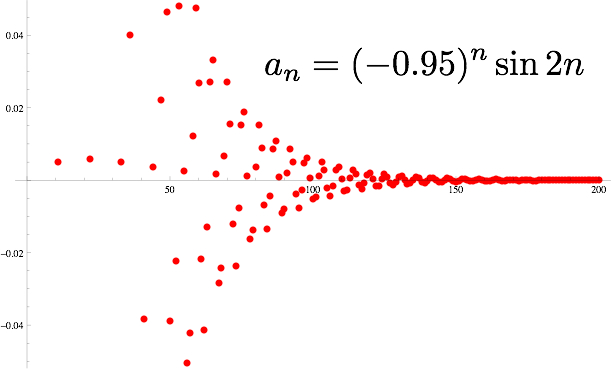
\includegraphics{./images/ch2/sin2nn.jpg}}
% 		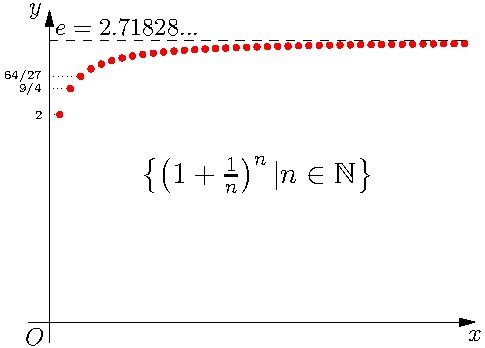
\includegraphics[width=6cm]{./images/ch1/e-notin-N}
	\end{center}
	根据常用极限\ps{稍后就会学到}
	$$e=\lim\limits_{n\to\infty}\left(1+\df1n\right)^n,$$
	不难看出$e=\mathrm{sup}A$。由于$e\notin\mathbb{Q}$,故有理数集不满足连续性公理。
	
	又比如下面的例子:
	
	{\bf 例:}$A=\{x\in\mathbb{Q}|x\geq 0,\;x^<2\}$,显然,
	$\mathrm{sup}A=\sqrt2\notin\mathbb{Q}$。
	
	{\bf 思考:}任给一个实数,如何构造一个有理数集合,使得该实数恰好为
	该有理数集合的上(下)确界?
	
	\begin{shaded}
	{\bf 开集与闭集}
	
	集合$A\subset\mathbb{R}$为{\bf 开集},是指:对任意$x\in A$,均存在$\delta>0$,使得
	$U(x,\delta)\subset A.$
	
	集合$A\subset\mathbb{R}$为{\bf 闭集},是指其补集$\bar{A}=\mathbb{R}-A$为开集。
	
	例如:所有的开区间都是开集,所有的闭区间为闭集;我们通常{\it 约定空集$\phi$既是开集又是闭集,
	因此{\b 实数集$\mathbb{R}$既是开集又是闭集}}。
	
	点$a$称为集合$A$的{\bf 内点},是指:存在$\delta>0$,使得$U(a,\delta)\subset A$。显然开集中的点均为其内点!
	
	点$a$称为集合$A$的{\bf 外点},是指:存在$\delta>0$,使得$U(a,\delta)\cap A=\phi$,
	或者说$a$为$A$的补给的内点。
	
	点$a$称为集合$A$的{\bf 边界点},是指$a$既不是$A$的内点,也不是$A$的外点,或者说
	对任意的$\delta>0$,$U(a,\delta)\cap A\ne\phi$。
	
	显然,闭集可以视为其最大开子集和其所有边界点的并。
	
	{\bf 例:}以下集合哪些是开集,哪些是闭集?
	\begin{enumerate}[(1)]
	  \setlength{\itemindent}{1cm}
	  \item $\{1,2,3,5\}$\quad\quad({\it 闭})
	  \item $U_0(1,3)$\quad\quad({\it 开})
	  \item 自然数集\quad\quad({\it 闭})
	  \item 有理数集\quad\quad({\it 既非开又非闭})
	  \item 无理数集\quad\quad({\it 既非开又非闭})
	  \item $\left\{\left(1+\frac
	  1n\right)^n|n\in\mathbb{N}\right\}+\{e\}$\quad\quad({\it 闭})
	\end{enumerate}
	
	\end{shaded}

\subsection{映射}

映射通常被定义为,事物之间“一对一”或“多对一”的依赖关系。更形象地说,可以将
映射视为一种输入输出过程,“一对一”或“多对一”保证了
一个输入只能得到一个特定的输出,因此结果是{\it 无歧义}
\ps{无歧义是保证数学论证简明性的一个常见的要求}
的。从这个意义上说,对于映射的这种定义方式也是一种{\it 约定}。
由集合$A$到$B$的映射$f$一般记为:

$$f:A\mapsto B \quad\mbox{或}\quad y=f(x),\;x\in A,y\in B$$

{\it 映射的三要素:}定义域、值域、对应关系,任何一项不明确都不足以确定一个函数,或者说,
两个映射在这三方面有一点不同,则应视为不同的映射。
\ps{之所以有时候只关心定义域和对应关系,前提是默认假设映射为满射}

{\bf 函数}通常是指实数集(的子集)之间的映射。有时也推广到高维的实数集,例如
$$z=x^2+y^2,\;(x,y)\in\mathbb{R}^2.$$

{\bf 例:}假设下列函数均取{\it 自然定义域}\ps{即在$\mathbb{R}$中最大的定义域},
且均为满射,指出其中哪些是完全相同的?
		$$x,\quad |x|,\quad e^{\ln x},\quad \ln(e^x),\quad \sqrt{x^2},\quad
		\frac{x^2-4}{x-2}-2,$$
		$$\sin(\arcsin x),\quad \arcsin(\sin x), \quad \tan(\arctan x)$$

相关概念:{\bf 单射、满射、一一映射(双射)}

\begin{shaded}
	{\bf 一一映射与无穷集合}
	
	{\bf 问题:}如何比较两个集合中元素的个数({\it 元素有限的情况下通常称为“度”})?
	
	答:如果存在集合$A$和$B$之间的一一映射,则称$A$和$B$是{\it 等势}的。
	
	{\bf 例:}以下集合两两等势吗,为什么?({\b 正确的命题须给出证明,错误的给出证明或举反例})
	\begin{enumerate}[(1)]
	  \setlength{\itemindent}{1cm}
	  \item 自然数与正偶数({$\surd$})
	  \item 自然数与整数({$\surd$})
	  \item 自然数与有理数({$\surd$})
	  \item 区间$(0,1)$中的实数与$\mathbb{R}$中({$\surd$},例如:$y=\df1{e^x+1}$)
	  \item 自然数与实数({$\times$})
	\end{enumerate}
	
	[提示]:(2)\;一个集合与自然数集等势,等价于这个集合中的所有数可以不重复地
	排成一列,形象地说,就是可以把这个集合中所有的数一个个地数完而没有任何重复
	与遗漏。例如要证明整数集与自然数集等势,显然只需这样来排列整数集:
	$$0,1,-1,2,-2,3,-3,4,-4,\ldots,$$
	很容易看出这样的排列是既没有遗漏也没有重复的,事实上等于给出了从自然数集到
	整数集的一一映射。
	
	(3)\;参照上面的作法,要证明自然数集与有理数集等势,也只需要考虑能否找到一种方式
	将所有的有理数排成一列,既不重复也不遗漏。参考下图,我们可以先说明所有的正有理数
	可以排成一列:
	\begin{center}
		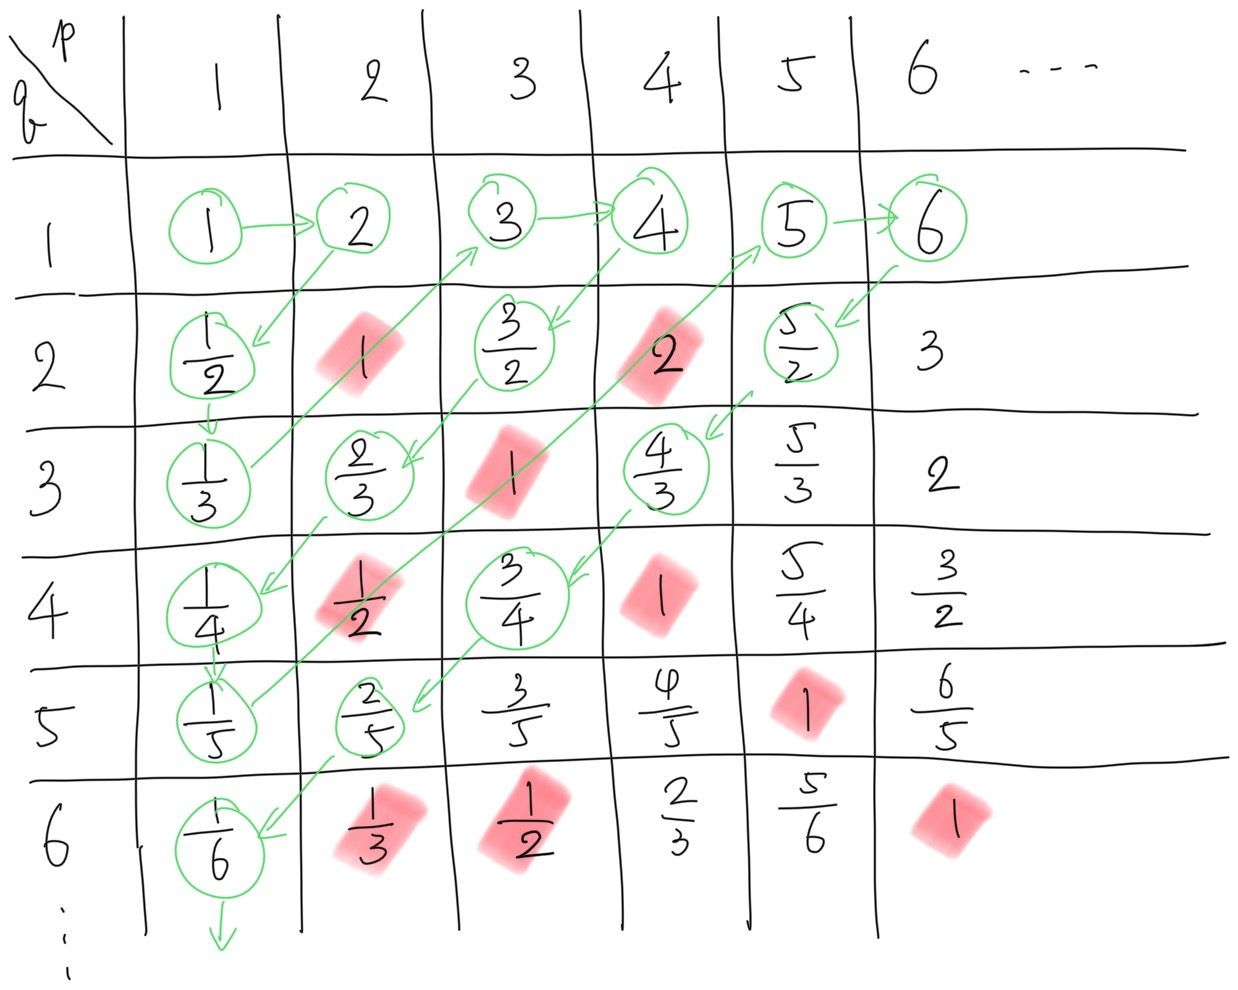
\includegraphics[width=8cm]{./images/ch1/Qp.jpg}
		
		{\it 表格中列出了所有的正有理数,红色覆盖的是重复出现的数字}
	\end{center}
	$$1,2,\df12,\df13,3,4,\df32,\df23,\df14,\df15,5,6,\df52,
	\df43,\df34,\df25,\df16,\ldots,$$
	从图上不难看出,这个排列事实上给出了从自然数集到正有理数集的一一映射。
	接下来,在其中逐个插入对应的负有理数,即可得到从自然数集到有理数集的
	一一映射。
	
	(5)\;了解了(4)的结论,我们只需证明不存在自然数集到区间$(0,1)$的一一
	映射即可。
	
	我们采用反证法:假设存在自然数集到$(0,1)$的
	一一映射,这意味着$(0,1)$中所有的数可以排成一个数列,没有重复也没有遗漏,
	其中第$i$个数表示为
	$$a_i=a_{i1}a_{i2}a_{i3}a_{i4}\ldots,$$
	其中$a_{ij}(j=1,2,\ldots)$都是$0$到$9$之间的个位整数。
	
	接下来,我们构造一个新的数
	$$a_*=a_{*1}a_{*2}a_{*3}a_{*4}\ldots,$$
	其中$a_{*j}(j=1,2,\ldots)$也都是$0$到$9$之间的个位整数,同时满足
	$$a_{*j}\ne a_{jj},\; j=1,2,3,\ldots.$$
	
	从$a_*$的构造特点上,我们可以得出如下两个结论:
	\begin{enumerate}[(i)]
	  \setlength{\itemindent}{1cm}
	  \item $a_*\in(0,1)$,
	  \item $a_*\ne a_i,\;i=1,2,3,\ldots$
	\end{enumerate}
	由于根据我们的假设,数列$\{a_i\}$中已经不多不少地包含了$(0,1)$中所有的数,因此
	以上第二条恰好说明$a_*\notin(0,1)$,这就出现了矛盾。从而可以断言
	假设错误,也就是说,不存在自然数集到$(0,1)$的一一映射,因此二者
	不等势,最终得到结论自然数集与实数集也不等势。
	
	上面这些结论反映出一个有趣的现象,就是有些集合可以和自己的真子集建立起
	一一映射。	Cantor敏锐地抓住了这一点,并认为应该是{\b\it 无穷集合}本质
	特征,进而第一次给出了无穷集合的概念,即:{\b 可以和自身的某个子集建立起
	一一映射的集合。}
	
	历史上,Cantor曾被人称为“{\it 数学史上最富于想象力的最具争议的人物之一}”、
	拥有“{\it 对于提出深刻的问题以及不时探索始料未及的解法以至寻求非正统答案的天赋}”。
	他的名言也是信条是“{\it 数学的本质在于它超然的自主性}”。
\end{shaded}	

	
\subsection{函数}
	
% 	\begin{shaded}
% 		{\bf 关于函数}
% 		\begin{itemize}
%   		  \setlength{\itemindent}{1cm}
% 		  \item 微积分是关于运动和变化的数学;
% 		  \item 函数是对运动(例如:曲线、曲面、波以及各种变化)变化过程中各种量与量的依赖关系的抽象描述;
% 		  \item 函数刻画了运动变化中的量之间的相互依存关系({\bf 注:}与“依存”对应的关系叫做“独立”)
% 		\end{itemize}
% 		
% 		{\bf 常量和变量}
% 		\begin{itemize}
%   		  \setlength{\itemindent}{1cm}
% 		  \item {\it 常量和变量是相对的},在一定条件下可以相互转化
% 		  \item 变量之间的关系可能是相互依存,也可能是相互独立的
% 		  \item 为了避免讨论过于复杂,简化问题,我们可能选择只考虑部分参数的变化,而将其他参数视为(或设为)常量,
% 		  例如:万有引力与两个物体的质量、距离以及引力常数(系数)都有关,为了确定其数量关系,需要事先假定部分的参数
% 		  值是固定不变的
% 		\end{itemize}
% 		
% 		{\bf 大学数学 vs. 中学数学}
% 		\begin{itemize}
%   		  \setlength{\itemindent}{1cm}
% 		  \item 数学并无严格的{\it “高等”}和{\it “初等”}之分,只是存在众多的分支和领域
% 		  (例如:代数、几何、分析、图论,几何又分为平面几何、立体几何、解析几何等),
% 		  不同分支或领域的直观性和难度各有不同
% 		  \item 对于函数,中学阶段更注重在对应关系“确定”的情况下,寻找其数学描述或利用给定的值进行计算
% 		  \item 大学阶段,从微积分开始,更着重对函数的特性(如导数、积分、曲率),
% 		  不同函数间的转换、类比,以及关于函数整体特征的计算与分析
% 		\end{itemize}
% 		
% 		 {\bf James Stewart, Calculus(5th eds.), 2004}
% 		  \begin{itemize}
%   		    \setlength{\itemindent}{1cm}
% 		    \item {\it Calculus is fundamentally different from the mathematics that
% 		    you have studied previously}
% 		    \item {\it Calculus is less static and more \underline{dynamic}
% 		    :微积分更加关注动态多余静止}
% 		    \item {\it It is concerned with change and \underline{motion}
% 		    :研究的对象是运动和变化}
% 		    \item {\it It deals with quantities that \underline{approach} 
% 		    other quantities
% 		    :关注数量之间的相互趋近}
% 		  \end{itemize}
% 	\end{shaded}
	
	函数是微积分研究的基本对象,不同于中学阶段,以对函数值的讨论和计算为重点,
	微积分更关注函数的变化特征(如导数与高阶导数、曲率)与整体性质(如连续性、
	定积分)。
	
	{\bf (一元)函数:}由实数集到实数集的映射
	$$f:D\mapsto\mathbb{R},\;(D\subset\mathbb{R})$$
	或
	$$y=f(x),\quad (x\in D\subset\mathbb{R},y\in\mathbb{R})$$
% 	\begin{itemize}
% 	  \item {\bf 定义域:} $D\subset \mathbb{R}$ ,且$D\ne\phi$ 
% 	  \item {\bf 对应关系:} $f:D\to\mathbb{R}$
% 	\end{itemize} 
	
	{\bf (一元函数的)函数图像:}
	$$G=\{(x,f(x))\in\mathbb{R}^2|x\in D\}$$
	
	\begin{shaded}
		{\bf 多元函数:} 
		$$f:D\to\mathbb{R},\quad D\in\mathbb{R}^n$$
		
		{\bf 向量值函数:}
		$$f:D\to\mathbb{R}^n,\quad, D\in\mathbb{R}$$
		
		{\bf 思考:}二元函数和三维的向量值函数可以表示怎样的几何对象?
	\end{shaded}
	
	\begin{center}
		\resizebox{!}{4.2cm}{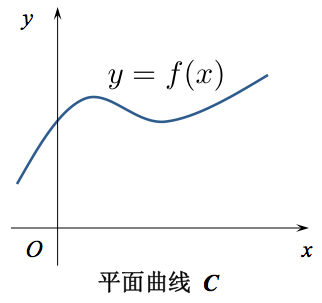
\includegraphics{./images/ch1/C_fx.jpg}}\quad	
		\resizebox{!}{4.5cm}{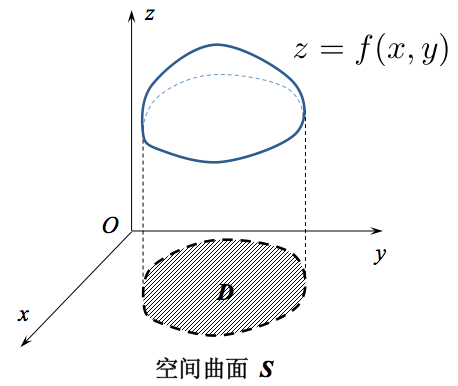
\includegraphics{./images/ch1/S_fxy.jpg}}
	\end{center}
	
	{\bf 思考:}{\b 平面曲线与一元函数具有一一对应关系吗?}空间曲面和二元函数呢?
	
	答:不是的,例如圆$x^2+y^2=1$如果写成一元函数形式,需要至少两个函数
	$y=\pm\sqrt{1-x^2}$。空间曲面和二元函数的关系与之类似,例如空间球面
	$x^2+y^2+z^2=1$也至少需要写成两个$z$关于$x,y$的二元函数
	$z=\pm\sqrt{1-x^2-y^2}$。
	
	由于以上问题的存在,为了表示平面曲线(空间曲面),我们会用到其他一些的曲线方程,
	例如:单位圆的方程也可以写为:\ps{关于参数方程和极坐标方程的介绍,参见KD教材1.3节}
	\begin{itemize}
%   		\setlength{\itemindent}{1cm}
		\item {\bf 隐函数方程}:$x^2+y^2=1$
		\item {\bf 参数方程}:$(x,y)=(\cos t,\sin t),\quad t\in[0,2\pi]$
		\item {\bf 极坐标方程}:$\rho=1,\theta\in[0,2\pi]$
	\end{itemize}
	
\subsubsection{函数的运算}

% {\bf 基本的函数运算}
% \ps{\b 因为无穷次的函数四则运算和复合可能导致一些特殊的函数性质出现,
% 以下如未特别说明,所列出的运算次数均为有限的}
\begin{enumerate}
  \setlength{\itemindent}{1cm}
  \item {\it 四则运算:}$+,-,\cdot,/$
  \item {\it 复合运算:}函数的复合运算就是中间变量的代入过程,$(f\circ g)(x)=f(g(x))$
  \item {\it 逆运算:}函数求逆(反函数)要注意反函数存在的条件:$f$为{\it 双射}
\end{enumerate}

{\bf 问:}$y=f(x)$和$x=f^{-1}(y)$的图形的关系是怎样的?({\it 答:相同!})

\subsubsection{函数的简单性质}
	
\begin{shaded}
	{\bf 常用的简写符号:}约定用于数学推导中一些常用文字的书写替代,汉英通用
	\begin{itemize}
	  \setlength{\itemindent}{1cm}
	  \item {\b$\bm{\forall}$} \quad 任意 (for all, arbitrary)
	  \item {\b$\bm{\exists}$} \quad 存在 (exist)
	  \item {\b$\bm{\Rightarrow}$} \quad 推出 (deduce, imply)
	  \item {\b$\bm{\Leftrightarrow}$} \quad 等价、当且仅当 (equivalent, if and only if)
	  \item {\b$\bm{\to}$} \quad 趋于 (approach)
	\end{itemize}
\end{shaded}

{\bf 【有界性】}			

	设$I\subset\mathbb{R}$,$f(x)$在$I$上有定义,若集合
	$\{f(x)|x\in I\}$	有界,则称{\it $f(x)$在$I$上有界}
	或{\it $f(x)$是$I$上的有界函数}
	\ps{函数的有界性就是其值域的有界性}

	{\bf 例:}判断以下函数在其定义域上的有界性
	\ps{注意掌握这几个函数图形的大致轮廓}
	
	\quad(1)\;$y=x\sin x$,\hspace{5em} (2)\;$y=\df{\sin x}x$,
	\hspace{5em} (3)\;$y=\sin\df1x$
		
	\begin{center}
		\resizebox{!}{4cm}{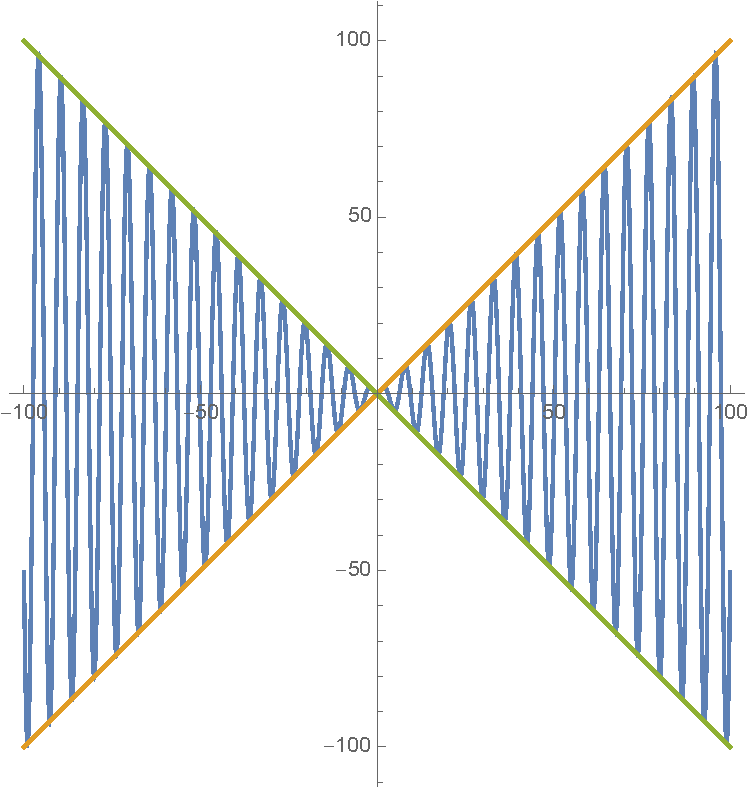
\includegraphics{./images/ch1/xsinx.pdf}}
		\resizebox{!}{3cm}{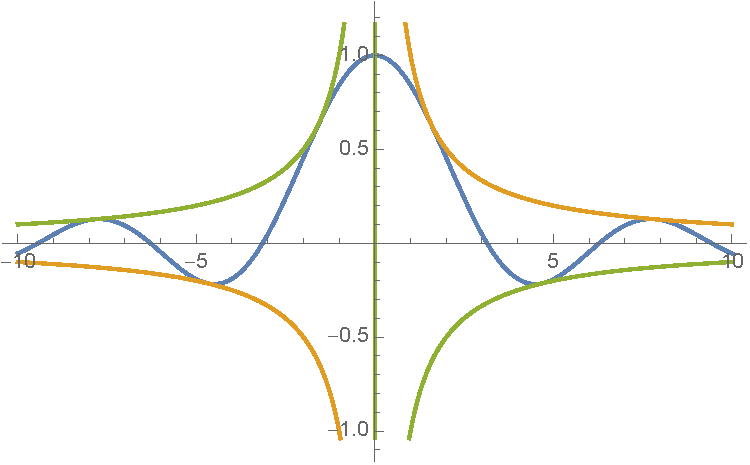
\includegraphics{./images/ch1/1xsinx.pdf}}	
		\resizebox{!}{3cm}{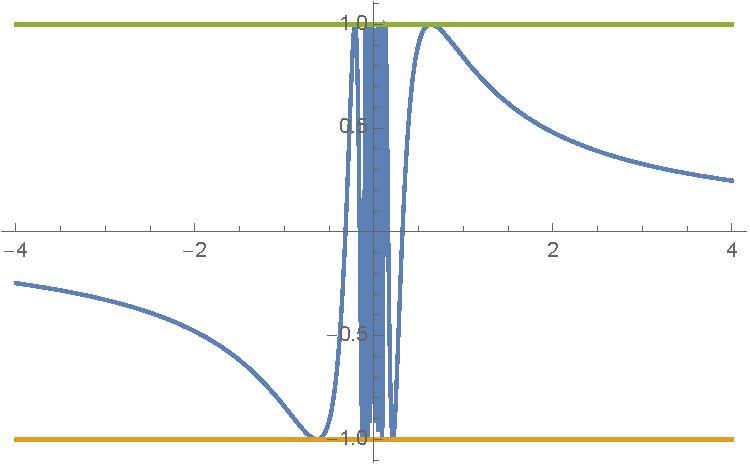
\includegraphics{./images/ch1/sin1x.pdf}}
	\end{center}
	
\begin{shaded}
	{\bf “反面定义”(否命题)的写法:}对命题中的如下文字进行相互替换
	\begin{enumerate}
	  \setlength{\itemindent}{1cm}
	  \item {\b “任意”与“存在”}
	  \item {\b “$\geq(\leq)$”与“$<(>)$”}
	  \item {\b “和”与“或”}
	\end{enumerate}
	
% 	[提示]::参考De Morgen律,任何命题的成立都是与一定范围有关的
	以函数的有界性为例,其否命题为函数无界。
	
	{\it $f(x)$有上界}:{\b\it 存在}$M\in\mathbb{R}$,对
	{\b\it 任意}$x\in D$,有$f(x){\b \leq} M$。
	
	{\it $f(x)$有上界}:对{\b\it 任意}$M\in\mathbb{R}$,{\b\it 存在}$x_M\in
	D$,使得$f(x_M){\b >}M$。
	
	{\bf 例:}用以上关于函数无上界的定义,证明$y=x\sin x$无界。
	
	注:所谓{\it 用定义证明}函数的性质,就是验证该函数满足这个定义中的命题
	
	[证]:对任意$M\in\mathbb{R}$,
	令$x_M=\left(\left[\df{M}{2\pi}\right]+1\right)
	\cdot2\pi+\df{\pi}2$(其中$[x]$为{\it 下取整函数},表示不大于$x$的最大整数,
	显然$[x]\leq x<[x]+1$),	则有
	$$x_M>\df{M}{2\pi}\cdot2\pi+\df{\pi}2>M,\quad\mbox{且}\quad \sin x_M=1,$$
	故
	$$x_M\sin x_M=x_M>M.$$
	从而根据函数无上界的定义,可知该函数无上界,从而无界。\hfill $\Box$
	
	注:有界是指既有上界又有下界,故无上界或无下界都可推出无界!
	
	{\bf 例:}证明:$f(x)=\df{\cos x}x$无界。
	
	[证]:对任意$M>0$,令$x_M=\min\left\{\df{\pi}4,\df1{2M+1}\right\}$,
	由于$x_M<\pi/3$时,$\cos x_M>\df12$,故
	$$f(x_M)>\df1{2x_M}>\df1{2\df1{2M+1}}=M+\df12>M,$$
	于是由定义可知,$f(x)$无界。\hfill $\Box$

	又比如数列极限的反面定义:

	{\it 数列$\{a_n\}$以$A$为极限:}任意$\e>0$,存在$N$,对任意
	$n>N$,满足$|a_n-A|<\e$

	{\it 数列$\{a_n\}$不以$A$为极限:}存在$\e_0>0$,对任意$N$,
	存在$n_0>N$,满足$|a_{n_0}-A|\geq\e_0$
\end{shaded}		

{\bf 【单调性】}

设$f:I\mapsto\mathbb{R}$,若对$\forall x_1,x_2\in I$,总有
$$x_1<x_2\Rightarrow f(x_1)\leq f(x_2)$$
则称{\it $f(x)$在$I$上单调递增}(若不等式中的等号总是无法成立,则称为
{\it 严格单调递增})
	
{\b{\bf 例:}证明函数$f(x)=x+\sin x$严格单调递增。}

\begin{center}
	\resizebox{!}{5cm}{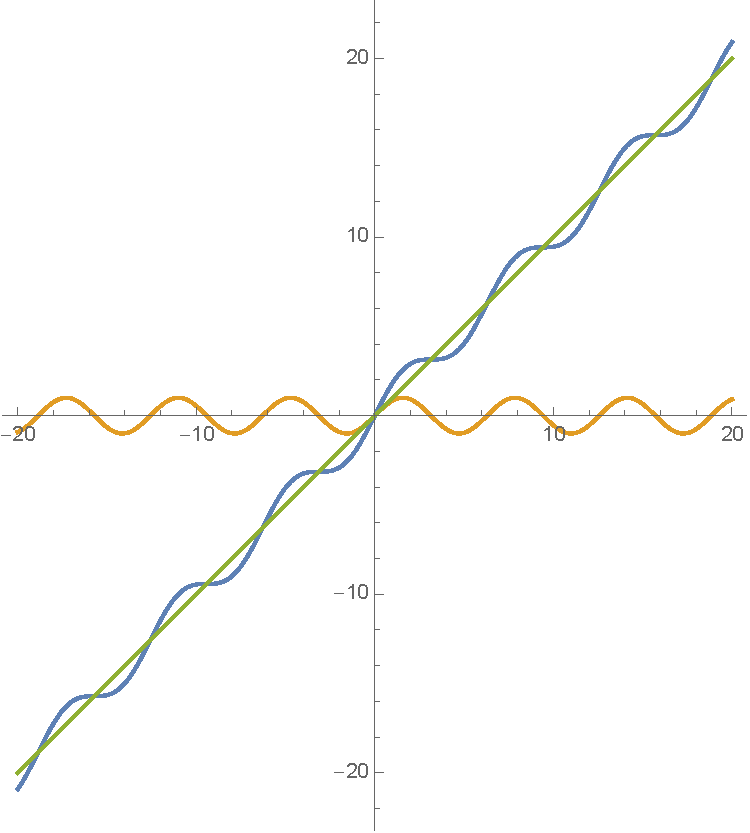
\includegraphics{./images/ch1/xpsinx.pdf}}
\end{center}

[证]:该函数的定义域为$\mathbb{R}$,任取$x_1,x_2\in\mathbb{R}$,则
$$f(x_2)-f(x_1)=(x_2-x_1)+2\sin\df{x_2-x_1}{2}\cos\df{x_2+x_1}{2}.$$

若$x_2-x_1>2\pi$,则由$\sin\df{x_2-x_1}{2}\cos\df{x_2+x_1}{2}\geq -1$,可得
$$f(x_2)-f(x_1)>(x_2-x_1)-2>2\pi-2>0;$$

若$0<x_2-x_1<2\pi$,注意到$|\sin x|<x\;(x>0)$,则有
$$f(x_2)-f(x_1)>(x_2-x_1)-2\left|\sin\df{x_2-x_1}{2}\right|
>(x_2-x_1)-2\df{x_2-x_1}{2}=0.$$

综上所述,对任意$x_2>x_1$,恒有$f(x_2)-f(x_1)>0$,故$f(x)$严格单调递增。
\hfill $\Box$


{\b{\bf 问:}严格单调的函数一定是一一映射,故一定存在反函数。如果反之,
存在反函数的函数一定会严格单调吗?}
\ps{要说明一个命题不成立,只需举出反例即可}

[答]:反之不成立。例如函数
$$f(x)=\left\{\begin{array}{ll}
	x,&0<x<1;\\
	3-x,&1\leq x<2
\end{array}\right.$$
的反函数就是其自身,但在定义域上不是单调的。

进一步思考:以上反例中的函数在每个连续的区间(例如$(0,1)$)上仍然是严格单调的,
这是函数存在反函数的必要条件吗?换句话说,是否存在某个函数存在反函数,
却在任意的区间上都不单调呢?

{\b {\bf 思考:}若对任意$x_1,x_2$,总有
$$[f(x_2)-f(x_1)](x_2-x_1)\leq 0,$$
可以推断$y=f(x)$具有何种性质?}
[答]:$y=f(x)$单调递减。

{\bf 【奇偶性】}

	设函数$f:D\mapsto\mathbb{R}$,{\it 称$f(x)$为偶(奇)函数},是指:
	对任意$x\in D$,有$f(-x)=f(x)\quad(f(-x)=-f(x))$

奇偶性是对称性的一种特例,由奇偶性的定义,很容易得到关于函数对称性的一些定义:

{\bf 例:}试给出如下性质的数学定义
\begin{enumerate}[(1)]
  \setlength{\itemindent}{1cm}
  \item {\b 函数$y=f(x)$的图像关于$x=a$对称
  \dotfill$f(2a-x)=f(x)$}
  \item {\b 函数$y=f(x)$的图像关于点$(x_0,y_0)$对称
  \dotfill $f(2a-x)=2f(a)-f(x)$}
\end{enumerate}

{\b {\bf 思考:}$f(x)=g(a-x),\;(x\in\mathbb{R})$有什么几何意义?

[答]{\it $f(x)$和$g(x)$的图像关于$x=a/2$对称!}}

{\bf 例:}$\sin x=\cos(\pi/2-x)$,
故可知$\sin x$和$\cos x$的图像关于$x=\pi/4$对称。

{\bf 定理:}{\b 任意一个定义在对称区间上的函数均可以表示为一个偶函数和一个奇函数的和},即
$$f(x)=\df{f(x)+f(-x)}{2}+\df{f(x)-f(-x)}{2}.$$
例如:
$$e^x=\df{e^x+e^{-x}}2+\df{e^x-e^{-x}}2$$

{\bf 【周期性】}

设函数$f:\mathbb{R}\to\mathbb{R}$,
称{\it $f(x)$为周期函数},是指: 存在$T>0$,
使对任意$x\in\mathbb{R}$,有
$f(x+T)=f(x)$。
满足以上性质的最小正数$T$称为$f(x)$的{\it 最小正周期}。
		 
{\bf 注:}若$T$为$f(x)$的一个周期,则任意$n\in\mathbb{Z}$和
任意$x\in\mathbb{R}$,总成立
$$f(x+nT)=f(x).$$

\subsubsection{常用函数}

{\bf 【符号函数】}

  $${\b \bm{\mathrm{sgn}}\,x =\left\{
	\begin{array}{rl}
	-1,\;&x<0 \\
	0,\;&x=0 \\
	1,\;&x>0
	\end{array}
  \right.}$$
显然,{\b $|x|=x \cdot\mathrm{sgn} x$}
	
{\bf 【(下)取整函数(阶梯函数)】}

  $${\b y=\left[ \,x\, \right]}$$
  $[\,x\,]$表示小于等于$x$的最大整数

{\bf 性质:}
\begin{enumerate}[(1)]
  \setlength{\itemindent}{1cm}
  \item {\b $[x]\leq x<[x]+1$}
  \item {\b $[x+1]=[x]+1$}
\end{enumerate}

{\bf 例:}试给出以下曲线的方程

\begin{center}
	\resizebox{!}{2.5cm}{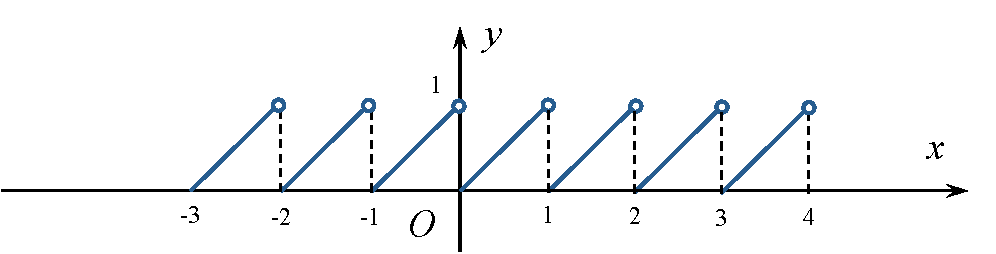
\includegraphics{./images/ch1/f1.pdf}}\quad $y=x-[x]$\\

	\resizebox{!}{2.5cm}{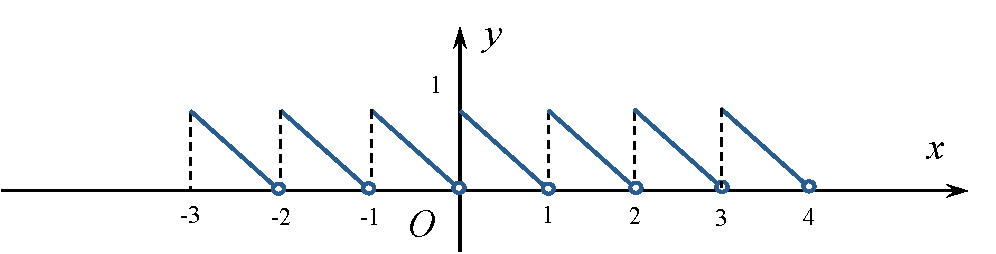
\includegraphics{./images/ch1/f2.pdf}}\quad $y=[x]-x+1$\\

	\resizebox{!}{2.5cm}{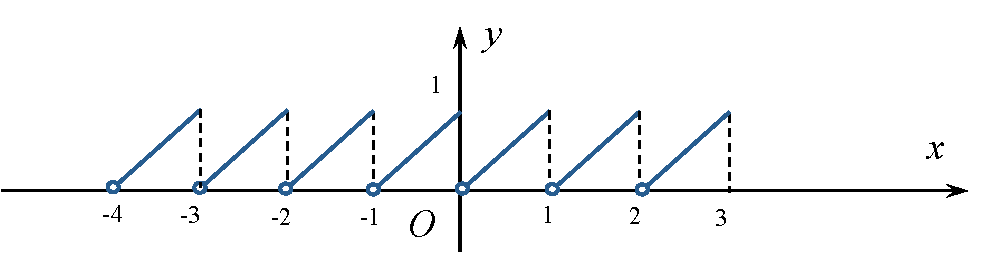
\includegraphics{./images/ch1/f3.pdf}}\quad $y=[-x]+x-1$
\end{center}
	
{\bf 例:}$(-1)^{[x]}$的图像?\quad({\it 方波!})

{\bf 例:}{\it 三角波}
$$y=\left|x-2\left[\df x2\right]\right|
\quad\mbox{或者}\quad
y=\df1{\pi}\arccos(\cos\pi x)$$

\begin{center}
	\resizebox{!}{2cm}{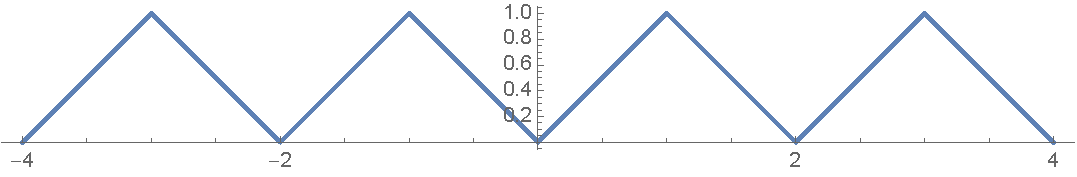
\includegraphics{./images/ch1/trif.pdf}}
\end{center}

{\bf 例:}证明:$f(x)=x-[x]$是以$1$为最小正周期的周期函数。\ps{参见MOOC第四讲}

{\bf 【Dirichlet函数】}
  $${\b \bm{D}(x) =\left\{
  \begin{array}{ll}
  	1,\;& x\in\mathbb{Q} \\
  	0,\;& x\notin\mathbb{Q}
  \end{array}
  \right.}$$
  {\bf 性质:}\ps{在后续章节中加以证明}
  \begin{enumerate}[(1)]
    \setlength{\itemindent}{1cm}
    \item $D(x)$在实数轴上处处无极限
	\item $D(x)$在实数轴上处处不连续
	\item {\it 仅在$x=0$这一点连续的函数:}$y=xD(x)$
	\item {\it 仅在$x=0$这一点可导的函数:}$y=x^2D(x)$
  \end{enumerate}

{\bf 【Riemann函数】} :\ps{这个函数也被称为“直尺函数”,最初由卡尔$\cdot$托梅提出}
设$x\in[0,1]$,
  $$\bm{R}(x) =\left\{
	\begin{array}{ll}
	1,\;&x=0\\
	\displaystyle\frac 1q,\;&x=\displaystyle\frac pq,\,p,q\mbox{互素}\\
	0,\;&x\notin\mathbb{Q}
	\end{array}
  \right. $$
  {\bf 性质:}
  \begin{itemize}
    \item 对任意$x_0\in[0,1]$, $\lim\limits_{x\to x_0}R(x)=0$
    \vspace{1ex}
    \item $R(x)$在{\it 无理数点连续, 有理数点不连续}
    \item $R(x)$是Riemann可积的
  \end{itemize}

{\bf 【初等函数】}

五类{\it 基本初等函数}:

\begin{enumerate}
  \setlength{\itemindent}{1cm}
  \item {\it 幂函数:} $y=x^a,\; (a\in\mathbb{R})$
  \ps{只有整数次幂的函数可以手工计算!!!}
  \item {\it 指数函数:} $y=a^x,\; (a>0,a\ne 1)$
  \begin{itemize}
    \item {$y=e^x$}
  \end{itemize}
  \item {\it 对数函数:} $y=\log_ax,\; (a>0,a\ne 1)$
  \begin{itemize}
    \item {$y=\ln x$}
  \end{itemize}
  \item {\it 三角函数:} $\sin x, \,\cos x,\, \tan x, \,\cot
  x,\, \sec x,\, \csc x$
  \item {\it 反三角函数:} $\arcsin x, \,\arccos x, \arctan x,
  \ldots$
\end{enumerate}

{\bf 问:}$\arcsin x$和$\arccos x$的定义域值域有何不同?
\ps{这是中学阶段需要了解的知识,不会的话自己好好补一补}

由常数和基本初等函数经过{\it 有限次}的四则运算和{\it 有限次}的函数复合
步骤所构成并{\it 可用一个式子表示}的函数,称为{\it 初等函数}

{\b 学习要求:熟练掌握五类基本初等函数的定义、图像、基本性质、各种运算公式(例如:
三角函数的和差化积、积化和差、半(倍)角公式、万能公式;反三角函数的定义域、值域、单调性;
一些常用的不等式,如$e^x-1>x>\ln(x+1)\;(x>0)$、平均值不等式、
$\sin x<x<\tan x\;(x>0)$等等。}

{\bf 例:}写出以下两个函数的表达式\ps{MOOC第五讲例1}
$$\arcsin(\sin x),\quad \sin(\arcsin x)$$

{\bf 例:}化简$\tan(\arcsin x),\;x\in(-1,1)$\ps{MOOC第五讲例2}

[解]:注意到
$$\tan x=\df{\sin x}{\cos x}=\df{\sin x}{\sqrt{1-\sin^2x}},$$
故
$$\mbox{原式}=\df x{\sqrt{1-x^2}},\quad x\in(-1,1).$$
\hfill $\Box$

{\bf 思考题:}证明:$\pi=20\arctan\df17+8\arctan\df3{79}$.

[提示]:等式两边都除以$4$,然后取正切,再反复利用
$$\tan(A+B)=\df{\tan A+\tan B}{1-\tan A\tan B}.$$

{\bf 【($n$次)多项式(函数)】}

{\b $$P_n(x)=\sum_{i=0}^na_ix^i,
  \quad (a_i\in\mathbb{R},a_n\ne 0,i=1,2,\ldots,n)$$
  {\bf 性质:}\ps{掌握结论,不要求了解证明}
  \begin{enumerate}[(1)]
    \setlength{\itemindent}{1cm}
    \item { $n$次多项式方程$P_n(x)=0$在$\mathbb{R}$上最多有$n$个根 (包含重根) ,在
    $\mathbb{C}$上有且仅有$n$个根(包含重根)};
    \item 设$x_i\in\mathbb{C}(i=1,2,\ldots,n)$为$P_n(x)=0$的全部根 ,则
    $$P_n(x)=a_n\prod_{i=1}^n(x-x_i)=a_n(x-x_1)(x-x_2)\ldots(x-x_n),$$
    \item 已知$P_n(x)$在$n+1$个点处的值, 可以唯一确定$P_n(x)$。
  \end{enumerate}
}

{\bf 【有理(分式)函数】}

$$f(x)=\frac{P(x)}{Q(x)}, \quad\mbox{其中}P(x),Q(x)\mbox{均为多项式函数}$$
  
{\bf 注:}{\b 任意有理函数总可以化为一个多项式函数和一个真分式(分子的次数比分母低的有理函数)
的和}
	  
{{\bf 例:}用多项式除法化简以下函数}
$$\frac{x^3+x^2-1}{x-1}=x^2+2x+2+\df{1}{x-1}$$
具体的除法过程如下,类似于小学学习过的竖式除法
\begin{center}
	{\b \polylongdiv{x^3+x^2-1}{x-1}}
\end{center}

{\bf 【双曲函数】}

{\small $$\sinh x =\df{e^x-e^{-x}}{2}, \quad
\cosh x =\df{e^x+e^{-x}}{2}, \quad\tanh x=\df{\sinh
x}{\cosh x}, \ldots$$}
{\bf 注:}双曲函数在很多场合也写作$\mathrm{ch}(x)$和$\mathrm{sh}(x)$
\ps{运算规律参见KD教材}

\section{数列的极限}

极限概念的引入是微积分发展史上具有革命性的一步,为奠定微积分理论“无可非议”的扎实
基础提供了可能。后续我们将要学习的导数、积分、级数等重要概念都是以极限的形式定义的。

数列极限是极限问题中最为简单的一类,也是性质非常典型的一类,可以作为我们后续学习
函数极限的基础。

{\bf 数列:}按一定规律排列的无穷多个(相同或不相同的)数,记作:
\ps{\b 有序性是数列最重要的特征,改变了数列中数的排列顺序将得到不同的数列}
$$a_1,a_2,\ldots,a_n,\ldots$$
或者$\{a_n\}$。

$\{a_n\}$的实质是定义在$\mathbb{N}_+$上的函数,因此也被称为
{\it 整标函数}或{\it 整序函数}。

如果在平面直角坐标系内作图,也可以将其视为一个动点随$n$增大所留下的离散的运动轨迹。

{\bf 思考:}数列与集合有哪些区别?\ps{1、有序-无序;\\ 2、无限-可能有限;\\ 3、可重复-不可重复}

{\bf 例:}数列举例

\begin{enumerate}[(1)]
  \setlength{\itemindent}{1cm}
  \item[(1)] $\left\{\df{n+1}n\right\}:\df 21,\df 32,\df43,\df54,\df65,\ldots$
  \item[(2)] $\left\{\df{(-1)^n}n\right\}:-1,\df12,-\df13,\df14,-\df15,\df16,\ldots$
  \item[(3)] $\{n^2\}:1,4,9,16,25,36,\ldots$
  \item[(4)] $\left\{n^{(-1)^n}\right\}:1,2,\df13,4,\df15,6,\ldots$
\end{enumerate}

\subsubsection{数列极限的定义}

形象地说,数列$\{a_n\}$的{\bf 极限}
\ps{现实生活里的极限更类似于我们所说的上限(确界)和下限(确界),例如:人类速度的极限}
,就是$a_n$的值随$n$的不断增大而趋向的某个确定的值,
当然,对于不同的$\{a_n\}$,这个确定的值不一定都存在!例如:
\begin{itemize}
  \item $\left\{\df1n\right\}$
  的值随着$n$不断增大会越来越趋近于$0$,因此其极限为$0$;
  \item $\{n\}$的取值会越来越大,甚至可以超过任何事先给定给定的值,
  因此也不会趋于任何确定的值,极限不存在;
  \item $\{(-1)^n\}$的取值在$1$和$-1$上反复交替,从整体上看,
  既不能说它趋近与$1$,也不能说它趋近于$-1$,所以极限也不存在。
\end{itemize}

在直观理解的基础上,我们集中来关注一个问题,即:{\it 数学上如何表达这种
趋向某个确定值的特征,或者说,如何给出数列极限的数学定义?}

以下的定义由数学家Weierstrass最终完成(注意,不是发明)\ps{现行的极限符号
$\lim$据说由数学家Hardy(1877-1947)引入,而最初提出通过引入极限来解决
微积分理论不严密问题的人是法国数学家d'Alembert}
,是被数学界最广泛接受的一种极限定义:

对于数列$\{a_n\}$,若存在常数$a$,{\b 对任意$\e>0$(不论它有多小),
都存在$N\in\mathbb{Z}_+$,使对任意$n>N$,都有
$$|a_n-a|<\e$$
成立},
%\ps{可简写为:$\forall\e>0,\exists N,\forall n>N,|a_n-a|<\e$}
则称{\it 数列$\{a_n\}$存在极限(或收敛)},常数$a$称为该数列的极限,记为
$$\b\lim_{n\to\infty}a_n=a$$
或\ps{\b 使用后面一种记号时,必须要写上$(n\to\infty)$}
$$\b a_n\to a\;(n\to\infty)$$
若上述常数$a$不存在,则称{\it 数列$\{a_n\}$不存在极限}(或{\it 发散})。

从几何上看(如下图所示),数列$\{a_n\}$以$a$为极限,意味着随着$n$的增大,$a_n$可以无限地
靠近$a$。为了表达这种“无限靠近”,数学上可以这样来解释:对于以$a$为中心的任意小的邻域$(a-\e,
a+\e)$(图上的蓝色阴影部分),只要把$n$取得充分大($N$的意义就是为了界定这个所谓的充分大
\ps{\b 显然,$\e$取得越小通常意味着$N$要取得越大,但必须注意的是$N$和$\e$
之间并不是简单的函数对应关系,因为如果某个$N$可以满足命题要求,
则$N$加任意的正常数显然也满足}
),则$a_n$都将落在$(a-\e,a+\e)$之内
\ps{\b 除了有限多个$a_n$外(准确地说是除了至多$\{a_n\}$的前$N$项外)}
。

\begin{center}
	\resizebox{!}{3cm}{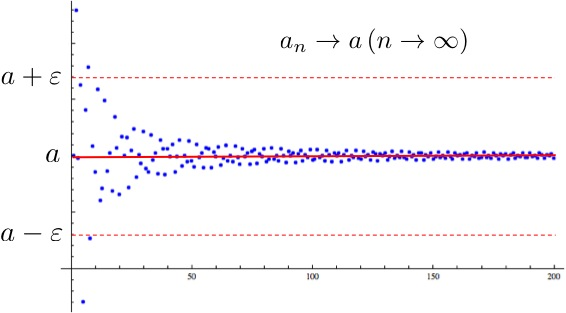
\includegraphics{./images/ch2/lim-en/en1.jpg}}\quad
	\resizebox{!}{3cm}{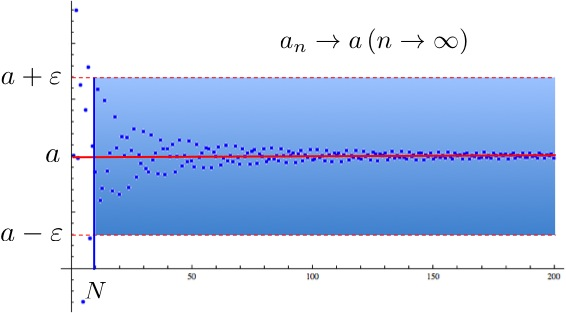
\includegraphics{./images/ch2/lim-en/en2.jpg}}
	
	\resizebox{!}{3cm}{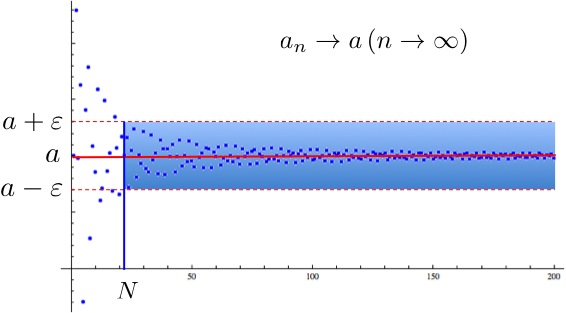
\includegraphics{./images/ch2/lim-en/en3.jpg}}\quad
	\resizebox{!}{3cm}{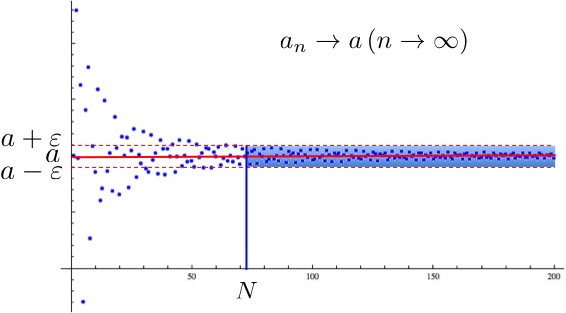
\includegraphics{./images/ch2/lim-en/en4.jpg}}
% 	
% 	\resizebox{!}{3cm}{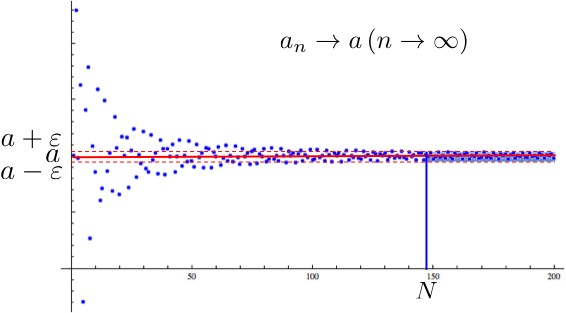
\includegraphics{./images/ch2/lim-en/en5.jpg}}
\end{center}

\begin{shaded}
	关于极限的定义,历史上曾经有过很长时间的讨论,当时的许多数学家都尝试
	过给出一个“合适”的极限定义,例如:Cauchy是这样描述极限的:
	
	{\kaishu
		当属于一个变量的相继值无限地趋近某个固定值时,如果以这样一种方式告终,
		变量值同固定值之差小到我们希望当任意小,那么这个固定值就成为其他所有值的极限。
	}
	
	这个定义中所描述的“趋近”这个行动,很难说是一种令人满意的表达方式。趋近是指
	一种实际的动作吗?如果是,是否意味着我们在讨论极限时,必须把时间和空间的概念
	包含在内?此外,什么才是这个过程的“告终”?
	
	相对而言,Weierstrass的极限定义里,没有任何动作,不涉及任何时间,完全
	是一个“{\it 静态的而非动态的定义}”,同时又是一个“{\it 代数的而非几何的定义}”。
	定义的核心是一个关于不等式的断言(命题)。最重要的是,利用它能够很容易地
	证明各种关于极限的定理,例如“和的极限等于极限的和”、“极限的保号性”。
	至此,对于类似的定理终于可以像Euclid的几何命题一样完全地严格化了。
	这是微积分发展历史上一个巨大的进步。
	
	Weierstrass被称为“{\it 现代分析学之父}”,《微积分的历程》一书这样评价他:
	{\kaishu
		19世纪,数学家们将微积分的严格性提高到一个新的水平。然而,按照我们今天的标准,
		这些成就并不是无可挑剔的。当你拜读那个时期的数学文献时,犹如聆听音乐大师肖邦
		在一架三两琴键失调的钢琴上演奏乐章,固然能够怡然自得地鉴赏音乐的神韵,不过
		间或也会听到些许畸变之音。只有在微积分中消除不精确的最后痕迹,分析论证变成对于
		一切实用目的都是无可置疑的时候,数学的新纪元才能到来,Weierstrass正是
		实现这个最后转变的最大功臣。 
		
		\ldots\ldots
		
		Weierstrass学派通过Weierstrass本人或者他的门生们发表的研究成果,对分析学
		赋予逻辑上的一种无与伦比的精确性。他矫正了许多难以捉摸的错误概念,证明了大量
		重要的定理,并且构造出一个令数学家们惊叹不已的处处连续而又不可微的函数的反例。
	}
	
	Weierstrass同时还是一名出色的数学教育家,Hiene(1821-1881)和Cantor都是他的门生。
\end{shaded}
	
前述定义更为简洁的写法:
\ps{\it\b 这种纯符号的表述方式固然简洁,但要正确掌握,
必须首先对更完整的文字表述有准确的理解,否则不建议随意使用}
$${\b \forall\e>0,\exists N\in\mathbb{Z}_+,\forall n>N,|a_n-a|<\e}\eqno{(1)}$$

{\bf 讨论:}以下说法和$(1)$等价的是:

\begin{enumerate}
  \setlength{\itemindent}{1cm}
%   \item[(2)] $\forall\e>0$,$\exists N>0$,$\forall
%   n>N$,$|a_n-a|<\e$ \hfill{$\surd$}\\
%   \hfill(直接写$\exists N$即可)
  \item[(2)] $\forall\e>0$,$\exists N$,$\forall
  n>N$,$|a_n-a|\leq\e$ \hfill{$\surd$} 
  
  \quad [提示]:只要强调$n>N$为正整数即可,根据需要$N$总是可以取得更大,
  无所谓是不是正整数。
  \item[(3)] $\exists N\in\mathbb{Z}_+$,$\forall\e>0$,$\forall
  n>N$,$|a_n-a|<\e$ \hfill{$\times$}
  
  \quad [提示]:(3)可以推出(1),但反之不然。事实上,由(3)可以推出,
  $\{a_n\}$仅有有限项的值不等于$a$,但显然不是所有收敛的数列都有此
  性质,例如$\{1/n\}$
  \item[(4)] $\forall\e>0$,仅有有限多个$n$,使得$|a_n-a|\geq\e$
  \hfill{$\surd$}
  
  \quad [提示]:由(4),仅有有限多个$a_n$不满足$|a_n-a|<\e$,则我们总可以取
  其中下标最大的下标作为$N$,则当$n>N$时,总有$|a_n-a|<\e$,即(1)成立;反之,由
  (1),最多有不超过$N$个$a_n$不满足$|a_n-a|<\e$,故(4)成立。
  
  \item[(5)] $\forall\e>0$,总有无穷多个$n$,使得$|a_n-a|<\e$
  \hfill{$\times$} 
  
  \quad [提示]:考虑反例:$a_n=(-1)^n$,取$a=1$。
  \item[(6)] $\forall\e>0$,要使$|a_n-a|<\e$,只须$n$充分大 \hfill{$\surd$}
  
  \quad [提示]:语序有变化,但逻辑关系和含义并未发生改变。
  \item[(7)] $\forall\e>0,\exists N\in\mathbb{Z}_+,\forall
  n>N,|a_n-a|<2\e$\hfill{$\surd$}
  
  {\quad\b\kaishu [注]:由于$\e$是任意的,$2\e$和$\e$的取值范围并没有区别,都是
  $(0,+\infty)$!事实上,在用定义证明极限时,完全可以使用$C\e$,
  其中$C\in\mathbb{R}$为给定的常数,这是数列极限最常用的一种等价定义。}
\end{enumerate}

{\bf 例:}证明:
$$\limn(-1)^n\df1{n^2}=0$$

[证]:对任意$\e>0$,{\b 令$N=\left[1/\sqrt{\e}\right]+1$}
\ps{不要忘记:\b $[x]\leq x<[x]+1$}
,则对任意$n>N$,有
$$\left|(-1)^n\df1{n^2}-0\right|=\df1{n^2}<\df1{N^2}
<\df1{(\sqrt{\e})^2}=\e,$$
由极限的定义,即证。\ps{\b 用定义证明数列极限,说明$N$的存在性是关键,为此主要有两种方式:\\
1、直接给出$N$的取值,例如$N=1/\e$\\
2、利用已知极限间接说明$N$存在,如$N=N_1$}
\hfill $\Box$

{\bf 例:}证明:
$$\limn\left(\df n{n+1}\right)^2=1$$

[证]:对任意$\e>0$,{\b 令$N=\left[2/\e\right]+1$},则对任意$n>N$,有
$$\left|\left(\df
n{n+1}\right)^2-1\right|=\df{2n+1}{(n+1)^2}<\df{2(n+1)}{(n+1)^2}
<\df2{n+1}<\df2n<\df2N<\e,$$
由极限的定义,即证。\hfill $\Box$

{\bf 例:}证明:若$\limn a_n=a$,则$\limn|a_n|=|a|$

[证]:对任意$\e>0$,由$\limn a_n=a$可知,存在$N_1\in\mathbb{Z}_+$,
对任意$n>N_1$,有
$$|a_n-a|<\e.$$
于是{\b 令$N=N_1$},则对任意$n>N$,有\ps{\b 利用$N_1$的存在性间接说明了$N$的存在性}
$$||a_n|-|a||\leq|a_n-a|<\e,$$
由极限的定义,即证。\hfill $\Box$

{\bf 课堂练习:}证明:若$|q|<1$,则$\{q^n\}$收敛。

[提示]:令$N=\left[\log_{|q|}\e\right]+1$

% {\bf 思考:}已知$|q|>1$时,$\{q^n\}$发散,请问该如何证明?
% 
% {\bf 注:}利用有界性,也可以证明发散。

\begin{shaded}
	{\bf 【极限定义的反面说法】}
	
	参照上一节对反面说法的介绍,由数列$\{a_n\}$以$a$为极限的定义:
	$$\limn a_n= a\quad\Leftrightarrow\quad\forall\e_0>0,
	\exists N\in\mathbb{Z}_+,\forall n>N,|a_n-a|<\e_0$$
	可以写出{\it 数列$\{a_n\}$不以$a$为极限}的定义:
	$$\limn a_n\neq a\quad\Leftrightarrow\quad\exists\e_0>0,
	\forall N\in\mathbb{Z}_+,\exists n_0>N,|a_{n_0}-a|\geq\e_0$$
	
	下面用这个定义来证明几个例子:
	
	{\bf 例:}证明:$\limn\df 1n\neq 1$
	
	[证]:取$\e=\df12$,对任意$N\in\mathbb{Z}_+$,令$n_0=\max\{3,N+1\}>N$,
	从而
	$$\left|\df1{n_0}-1\right|=1-\df1{n_0}\geq 1-\df13=\df23>\e,$$
	由极限的反面定义,即证。\hfill $\Box$
	
	{\bf 例:}证明$\{(-1)^n\}$发散。
	
	[证]:任取$a\in\mathbb{R}$,只需证明$\limn(-1)^n\ne a$。以下不妨设$a>0$。
	
	取$\e=1$,对任意$N\in\mathbb{Z}_+$,令$n_0=\max\{2[N]+1,1\}>N$,则
	$$\left|(-1)^{n_0}-a\right|=|-1-a|=a+1>\e,$$
	由极限的反面定义,即证。\hfill $\Box$
	
	相对于使用的反证法,用反面定义证明极限不存在,形式上更简洁,但
	却不是特别直观和容易理解。
	
	需要提醒的是,数列不以某个值为极限和数列发散是两个不同的概念,后者意味着
	数列不以任何的值为极限。
	
	{\bf 思考:}数列发散可能有哪些不同的情形?\hfill({\it 趋向无穷,或反复振荡不收敛})
\end{shaded}

\subsubsection{数列极限的性质}

以下三个性质的证明,可以作为用极限定义证明命题的典型例子,应重点理解、掌握。

{\bf 唯一性:}数列极限若存在,必唯一。\ps{可以说,是唯一性的要求决定了当前的极限定义。
从这个意义上说,目前使用的极限定义其实也是一种约定。}
%“记录重大技术突破的技术发展史其实就是一部人类社会发展的技术选择史”

\begin{center}
	\resizebox{!}{4cm}{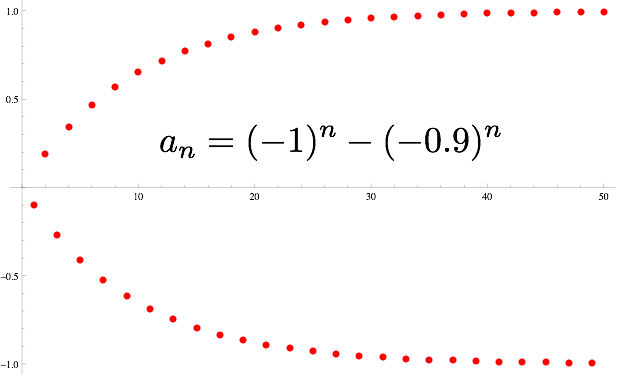
\includegraphics{./images/ch2/1-0.9n.jpg}}
	
	一个不收敛的数列
\end{center}

下面的证明需要用到如下的命题:设$a,b\in\mathbb{R}$,若对任意$\e>0$,
有$|a-b|<\e$,当且仅当$a=b$
\ps{\b 两个确定的数如果可以无限靠近(小于任意给定的距离),则意味着它们相等。}

[证]:设$a,b$均为数列$\{a_n\}$的极限。

对任意$\e>0$,由$\limn a_n=a$,存在$N_1\in\mathbb{Z}_+$,对任意$n>N_1$,有$|a_n-a|<\e$;

同理,由$\limn a_n=b$,存在$N_2\in\mathbb{Z}_+$,对任意$n>N_2$,有$|a_n-b|<\e$。

令{\b $N=\max\{N_1,N_2\}$},则当$n>N$时,有
$${\b |a-b|\leq|a_n-a|+|a_n-b|<2\e},$$
由此可知,必有$a=b$,即证。\hfill $\Box$

{\bf 有界性:}数列$\{a_n\}$若收敛,则{\it $\{a_n\}$有界},即:存在$M>0$,对任意
$n\in\mathbb{Z}_+$,恒有$|a_n|\leq M$。

\begin{center}
	\resizebox{!}{4cm}{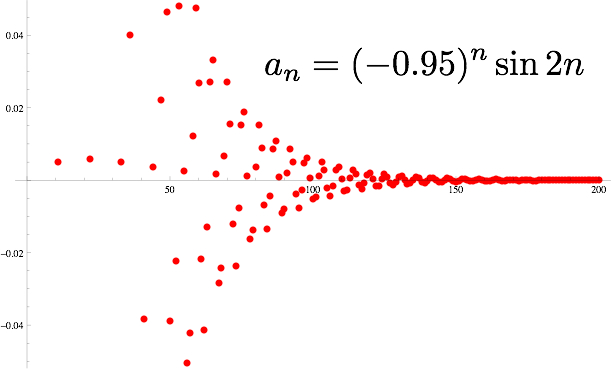
\includegraphics{./images/ch2/sin2nn.jpg}}
	
	一个收敛的数列
\end{center}

思路:{\b 利用$\e$的特定取值“控制”无穷的部分,剩余的有限多个数构成的集合自然是有界的}

[证]:记$\limn a_n=a$。由极限的定义,对{\b$\e=1$},存在$N\in\mathbb{Z}_+$,
对任意$n>N$,有
$$|a_n-a|<\e=1\quad\Rightarrow\quad |a_n|<|a|+1.$$
记{\b$M=\max\{|a|+1,|a_1|,|a_2|,\ldots,|a_{[N]+1}|\}$},则对
任意$n\in\mathbb{Z}_+$,均有
$$|a_n|\leq M,$$
即证。\hfill $\Box$

该性质的一个显然的推论是:{\b 如果数列无界,则必发散。}

{\bf 例:}讨论$\{\sqrt[n]{n!}\}$的敛散性。

思路:对任意$M>0$,当$n$充分大时,总有$n!>M^n$,故$\{\sqrt[n]{n!}\}$无界,
从而发散。

[证]:对任意$M>0$,令$N=[2M]+1$,则当$n>N$时,总有$n>2M$。此时
$$\df{n!}{M^n}=\df{N!}{M^N}\cdot\df{N+1}{M}
\cdot\df{N+2}{M}\ldots\df{n}{M}<\df{N!}{M^N}\cdot2^{n-N+1}.$$
注意到$\df{N!}{M^N}$为有限值,而$2^{n-N+1}$随着$n$的增大趋于正无穷,
故当$n$充分大时,必有
$$\df{n!}{M^n}=\df{N!}{M^N}\cdot2^{n-N+1}>1,$$
从而$\sqrt[n]{n!}>M$,也即$\{\sqrt[n]{n!}\}$无界,故发散。\hfill $\Box$

{\bf 保号性:}设$\lim\limits_{n\to\infty}a_n=a>0$,则存在$N$,
对任意$n>N$,$a_n>0$

[证]:由$\lim\limits_{n\to\infty}a_n=a>0$,对$\e=a/2$,存在
$N$,对任意$n>N$,
$$|a_n-a|<\e=a/2\quad\Rightarrow\quad \df32a>a_n>a/2>0,$$
即证。\hfill $\Box$
		
{\bf 保号性常见的几种形式(几个推论):}
\begin{enumerate}
  \setlength{\itemindent}{1cm}
  \item 对任意$n\in\mathbb{N}$,$a_n\geq
  0$, $\lim\limits_{n\to\infty}a_n=a$, 则$a\geq 0$
%    \ps{\b 保号性可以理解为极限运算保持不等号的方向不变,即:
%    若$\{a_n\}$收敛,则由$a_n\geq 0$可推出$\limn a_n\geq0$} 
  \item 设$\lim\limits_{n\to\infty}a_n=a\ne
  0$, 则$\exists N$,当$n>N$时,$|a_n|>|a|/2$
  \item  设$\lim\limits_{n\to\infty}a_n=a$, 且最多有有限
  个$a_n$小于零, 则$a\geq 0$
\end{enumerate}	

{\bf 注:}{\b 保号性的实质,是{\it 极限运算保持不等号的方向
\ps{但严格大(小)于可能变成大(小)于等于}不变},
若已知$\limn a_n=a,\limn b_n=b$,则
$$a_n\geq b_n\,(n\in\mathbb{Z}_+)\quad\Rightarrow
\quad\limn a_n\geq\limn b_n$$
}

{\bf 收敛数列与其子数列的关系:}数列$\{a_n\}$收敛,当且仅当它的所有
子列均收敛到相同的极限。

{\it 子数列:}从原数列中按一定顺序选取数,所构成的一个新的数列,通常记为
$\{a_{n_k}\}$,其中$\{n_k\}$是一个严格单调递增的正整数列。显然,
对{\b 任意$k\in\mathbb{Z}_+$,$n_k\geq k$。}

数列$\{a_n\}$的{\it 奇子列}和{\it 偶子列}可记为$\{a_{2k}\}$、$\{a_{2k-1}\}$,
有时也直接写为$\{a_{2n}\}$、$\{a_{2n-1}\}$。

{\it 子数列$\{a_{n_k}\}$以$a$为极限},
也即:对任意$\e>0$,存在$K\in\mathbb{Z}_+$,使对任意$k>K$,总有
$$|a_{n_l}-a|<\e.$$
记为\ps{强调$k$变化而不是$n$变化,事实上$n_k$可以视为整序函数的复合函数中的中间变量}
$$\b\lim\limits_{k\to\infty}a_{n_k}=a,\quad 
\mbox{或}\quad a_{n_k}\to a\;{(k\to\infty)}$$

下面证明上述性质:

[证]:充分性是显然的,因为$\{a_n\}$可以看成是自身的一个子列。

下面证明必要性。设$\limn a_n=a$,则对任意$\e>0$,存在$N\in\mathbb{Z}_+$,
使对任意$n>N$,有$|a_n-a|<\e$。

设$\{a_{n_k}\}$为$\{a_n\}$的任一子列。令$K=N$,则由$\{n_k\}$严格单调递增,
可知对任意$k>K$,都有$n_k>n_K\geq K=N$,从而 
$$|a_{n_k}-a|<\e.$$
也即$\lim\limits_{k\to\infty}a_{n_k}=a$。因为$\{a_{n_k}\}$是任意的,即证。
\hfill $\Box$

% 该性质的另一种表述方法:
% $$\limn a_n=a\quad\Leftrightarrow\quad
% \mbox{对任意严格单调递增的正整数数列}\{n_k\},
% \lim_{k\to\infty}a_{n_k}=a.$$

这个性质的一个明显用途,是判定一些数列的发散。

{\bf 例:}证明数列$\{(-1)^n\}$发散。

[证]:取该数列的欧子列和奇子列,分别即为$\{a_{2k}\}$和$\{a_{2k-1}\}$。显然,
对任意$k\in\mathbb{Z}_+$,都有
$$a_{2k}\equiv 1,\quad a_{2k-1}\equiv -1,$$
因此
$$\lim\limits_{k\to\infty}a_{2k}=1,\quad
\lim\limits_{k\to\infty}a_{2k-1}=-1.$$
由二者极限不相等可知原级数发散,即证。\hfill $\Box$

这种方法证明发散,比前面使用数列收敛的反面定义要更加简洁,也更加直观。

{\bf 例:}\ps{KD教材2.2.2节-例4}
证明数列$\left\{n^{(-1)^n}\right\}$发散。

[提示]:原数列存在发散子列$\left\{(2n)^{(-1)^{2n}}\right\}=\{2n\}$。

{\bf 例:}证明$\left\{\left(1+\df1{\sqrt n}\right)\sin\df{\pi\sqrt n}2\right\}$
发散。

[提示]:取$n_k=k^2$。 

\begin{shaded}
	{\bf 例:}证明:$\{\sin n\}$发散。
	
	[证一]:用反证法。设有$\limn\sin n=a$,则
	$$\limn[\sin(n+2)-\sin n]=0.$$
	进而由
	$$\sin(n+2)-\sin n=2\sin 1\cos(n+1),$$
	可得$\limn\cos(n+1)=0$。又
	$$\cos(n+1)=\cos n\cos 1-\sin n\sin 1,$$
	可得$\limn\sin n=0$。如此就有
	$$\limn\sin n=\limn\cos n=0,$$
	显然与$\sin^2n+\cos^2n=1$矛盾。\hfill $\Box$
	
	[证二]:注意到当$x\in[2k\pi+\pi/4,2k\pi+3\pi/4]\,(k\in\mathbb{N})$时,总有
	$$\sin x>\sqrt2/2.$$
	由于此类区间的长度均超过$1$,故其中必包含至少一个自然数。于是对每个$k\in\mathbb{N}$,
	可取自然数$n^{(1)}_k\in[2k\pi+\pi/4,2k\pi+3\pi/4]$,显然$\{\sin{n^{(1)}_k}\}$构成了$\{\sin
	n\}$的一个子列。
	
	若$\{\sin n\}$收敛,则$\{\sin{n^{(1)}_k}\}$也收敛,且与之极限相同。由极限的保号性,
	可知$\{\sin{n^{(1)}_k}\}$的极限不小于$\sqrt2/2$,从而$\{\sin
	n\}$的极限应大于等于$\sqrt2/2$。
	
	同理,利用区间$[2k\pi+5\pi/4,2k\pi+7\pi/4]\,(k\in\mathbb{N})$,可构造$\{\sin
	n\}$的另一个子列 $\{\sin{n^{(2)}_k}\}$。若$\{\sin n\}$收敛,同样利用保号性可证明其极限应小于等于$-\sqrt2/2$。
	
	以上两方面的结论矛盾,故假设错误,即证。\hfill $\Box$
\end{shaded}

该性质的一个常见推论称为{\it 拉链定理}:若某个数列的奇子列和偶子列收敛到相同的极限,
则该数列收敛。

请自行尝试证明该定理。此外,还请想一想,这个定理可以进一步推广吗?

{\bf 注:}更一般性的推广:如果选择的多个子列按顺序合并起来能够完全覆盖原数列,
或最多不能覆盖原数列中有限多个数,且这些子列均收敛于相同的极限,则原数列收敛。
例如:{\it 若子数列$\{a_{3n}\},\{a_{3n-1},\{a_{3n-2}\}\}$都收敛于$a$,
则$\{a_{n}\}$收敛于$a$。}

\begin{shaded}

{\bf 思考题:}证明:若$\limn a_n=a$,则$\limn\df{a_1+a_2+\ldots+a_n}n=a$。

[证]:对任意$\e>0$,由$\limn a_n=a$,存在$N_1$,对任意$n>N_1$,总有
$$|a_n-a|<\e.$$
记
$$M_{N_1}=|(a_1-a)+(a_2-a)+\ldots+(a_N-a)|,$$
显然$M_{N_1}$的值只与$N_1$有关,而与$n$无关,故令$N_2=\df{M_{N_1}}{\e}$,
则对任意$n>N_2$,总有
$$\df{M_{N_1}}{n}<\e.$$

至此,令$N=\max\{N_1,N_2\}$,则对任意$n>N$,均有
\begin{align*}
	&\left|\df{a_1+a_2+\ldots+a_n}n-a\right|\\
	&=\df1n|(a_1-a)+(a_2-a)+\ldots+(a_n-a)|\\
	&\leq\df1n\left[M_{N_1}
	+|(a_{N+1}-a)+(a_{N+2}-a)+\ldots+(a_n-a)|\right]\\
	&<\e+\df1n\left[|a_{N+1}-a|+|a_{N+2}-a|
	+\ldots+|a_n-a|\right]\\
	&<\e+\df1n(n-N)\e<2\e,
\end{align*}
由数列极限的定义,即证。\hfill$\Box$

这个结论也称为Cauchy{\it 极限定理},有着非常重要的应用,例如,今后我们会学习
下面的极限$\limn\sqrt[n]a=1,\,(a>0)$,于是立即可以得到
$$\limn\df1n(a+\sqrt[2]a+\sqrt[3]a+\ldots+\sqrt[n]a)=1.$$

此外,我们今后还会学习到极限运算和初等函数运算可以交换次序,进而可以证明如下的命题:

{\bf 例:}设$a_n$均大于零,且$\limn\df{a_{n+1}}{a_n}=q$,则
$\limn\sqrt[n]{a_n}=q$。

[证]:记$b_1=a_1$,$b_n=\df{a_n}{a_{n-1}}\;(n>1)$,则
% $$a_n=\df{a_n}{a_{n-1}}\cdot\df{a_{n-1}}{a_{n-2}}
% \cdots\df{a_2}{a_1}\cdot a_1$$
$$a_n=b_n\cdot b_{n-1}\cdots b_1,$$
进而
$$\ln a_n=\ln b_n+\ln b_{n-1}+\ldots+\ln b_1,$$
已知$\limn b_n=q$,根据初等函数的性质,可得$\limn\ln b_n=\ln q$,
于是由Cauchy极限定理,
$$\limn\ln \sqrt[n]{a_n}=\limn\df1n\ln a_n=\limn\df1n\left(
\ln b_n+\ln b_{n-1}+\ldots+\ln b_1\right)=\ln q,$$
进而可得$\limn\sqrt[n]{a_n}=q$。\hfill$\Box$

有了这个定理,我们很容易得到下面的结论:若$\limn a_n=a\geq 0$,则
$$\limn\sqrt[n]{a_1a_2\ldots a_n}=a.$$

\end{shaded}

\section{函数的极限}

\subsection{函数极限的定义}

函数极限是我们后续定义导数、积分的概念的基础。从形式上看,可以将它视为数列极限的推广,
但从直观意义上看,二者存在很大的不同。

不同于数列极限只有单一的$n\to\infty$一种(自变量的变化)趋势,
函数极限共有{\it 六种可能的(自变量变化)趋势},分为两大类:

\begin{itemize}
  \setlength{\itemindent}{1cm}
  \item {\it 自变量趋于无穷}
  $$\b x\to\infty,\quad x\to+\infty,\quad x\to-\infty$$
  \item {\it 自变量趋于有限值}
  $$\b x\to x_0,\quad x\to x_0^+,\quad x\to x_0^-$$
\end{itemize}

{\bf 思考:} $\limn f(n)=A\Leftrightarrow\limx{+\infty}f(x)=A$成立吗?

答:显然,{\b$\limx{+\infty}f(x)=A$可以推出$\limn f(n)=A$,但反之不然},
\ps{事实上,$f(n)$的值域是$f(x)$值域的子集}

例如:$y=\sin\pi x$当$x\to+\infty$时不收敛,但$\limn\sin n\pi=0$。

{\bf 【趋于无穷时的函数极限】}

{\bf 定义:}
\ps{\b 和$\limn a_n=a$的定义做类比,进行形式推广}
\begin{enumerate}[(1)]
  \setlength{\itemindent}{1cm}
  \item $\limx{+\infty}f(x)=A\Leftrightarrow\forall \e>0,\exists X,\forall
  x>X,|f(x)-A|<\e$
  \item $\limx{-\infty}f(x)=A\Leftrightarrow\forall \e>0,\exists X,\forall
  x<X,|f(x)-A|<\e$
  \item $\limx{\infty}f(x)=A\Leftrightarrow\forall \e>0,\exists X,\forall
  |x|>X,|f(x)-A|<\e$
\end{enumerate}

{\bf 注:}和数列极限类似,在函数极限的定义中,最后不等式右端的$\e$可以改写为$C\e$,
其中$C>0$为常数,所得命题与原定义等价。

{\bf 例:}证明$\limx{+\infty}\df1{\sqrt x}=0$.

[证]:对任意$\e>0$,取$X=\df1{\e^2}$,则对任意的$x>X$,都有
$$\left|\df1{\sqrt x}-0\right|=\df1{\sqrt x}<\df1{1/\e}=\e,$$
由函数极限的定义,即证。\hfill $\Box$

{\b 趋于无穷的函数极限存在,意味着函数存在{\it 水平渐近线}},需要注意的是,
水平渐近线最多可以有两条,例如:

% \begin{center}
% 	\resizebox{!}{4cm}{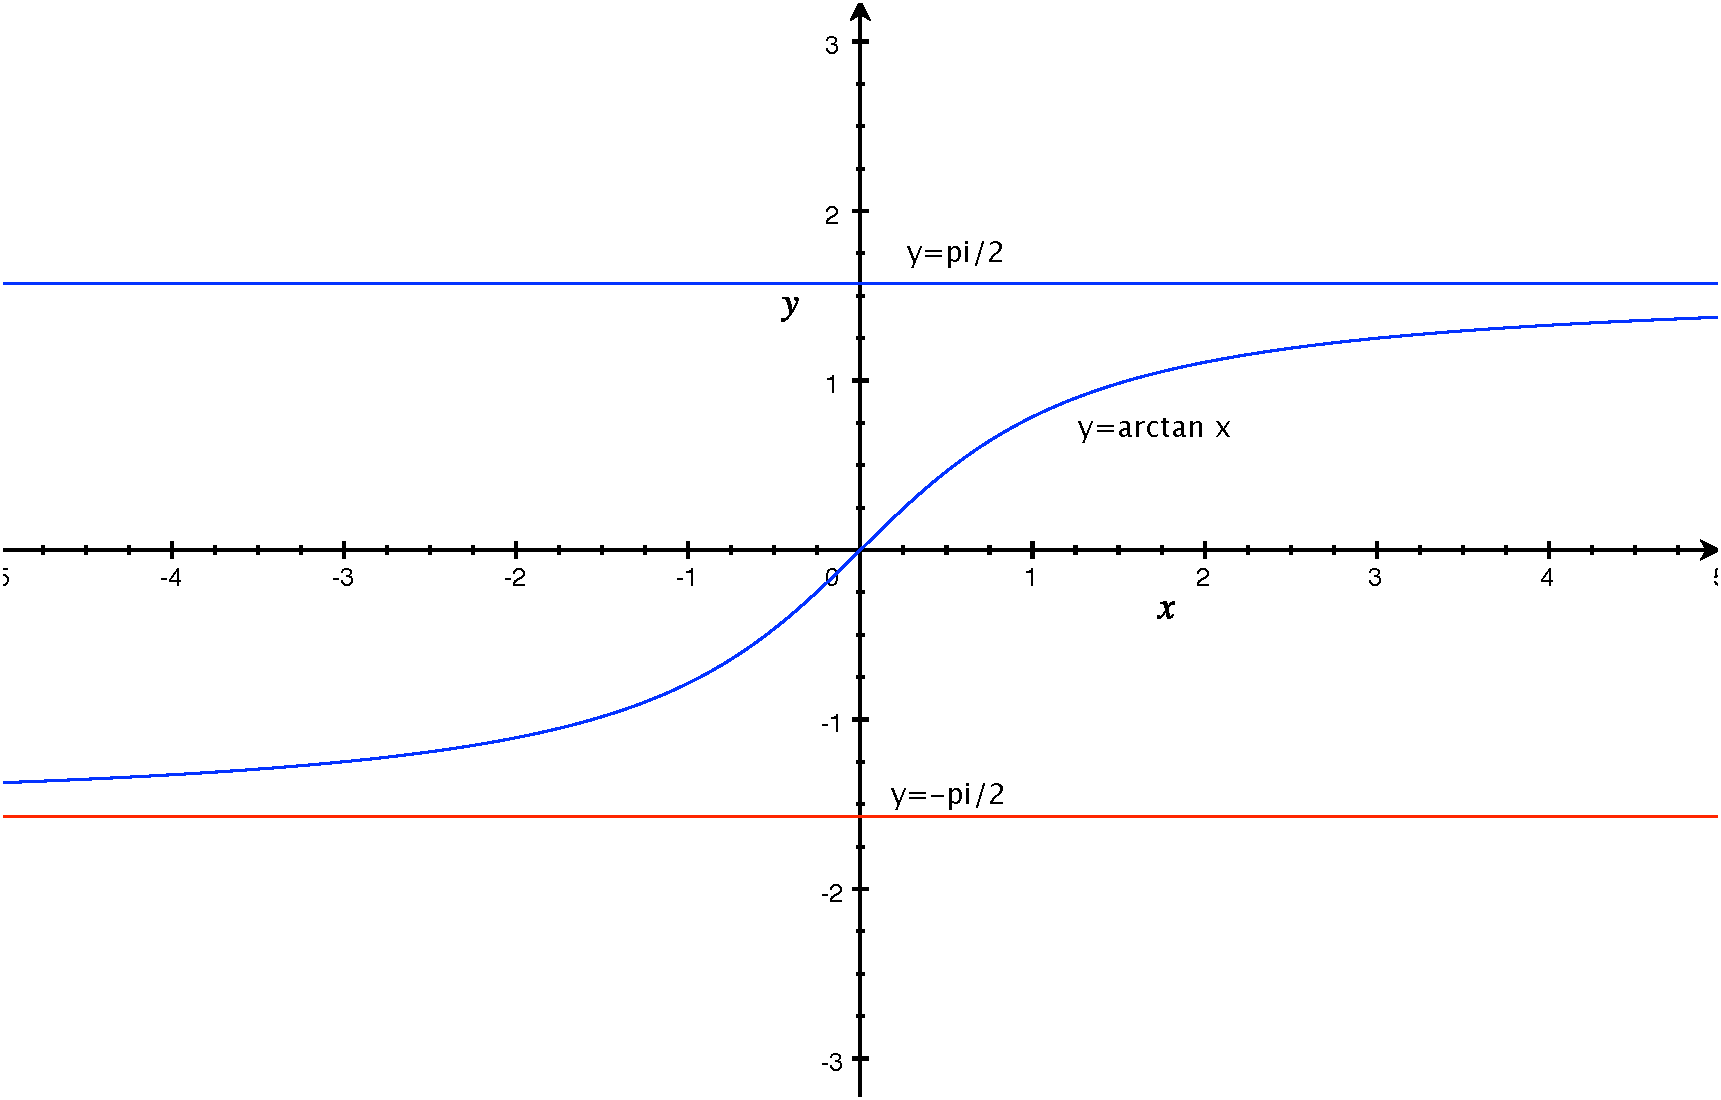
\includegraphics{./images/ch3/arctan.pdf}}
% \end{center}

\begin{center}
	\begin{overpic}[scale=0.3]{./images/ch3/arctan.pdf}
		\put(0,10){\b $\limx{-\infty}\arctan x=-\df{\pi}2$}
		\put(65,53){\b $\limx{+\infty}\arctan x=\df{\pi}2$}
	\end{overpic}
	
	$y=\arctan x$的图像与两条水平渐近线
\end{center}

{\bf 【趋于有限值时的函数极限】}

{\bf 定义:}
\begin{enumerate}[(1)]
  \setlength{\itemindent}{1cm}
  \item $\limx{x_0}f(x)=A\Leftrightarrow\forall \e>0,\exists\delta>0,\forall
  x\in U_0(x_0,\delta),|f(x)-A|<\e$
  \item $\limx{x_0^+}f(x)=A\Leftrightarrow\forall \e>0,\exists\delta>0,\forall
  x\in(x_0,x_0+\delta),|f(x)-A|<\e$
  \item $\limx{x_0^-}f(x)=A\Leftrightarrow\forall \e>0,\exists\delta>0,\forall
  x\in(x_0-\delta,x_0),|f(x)-A|<\e$
\end{enumerate}

{\bf 例:}\ps{KD教材习题3.1-1}
根据图形判断极限的存在性
\begin{center}
	\resizebox{!}{4cm}{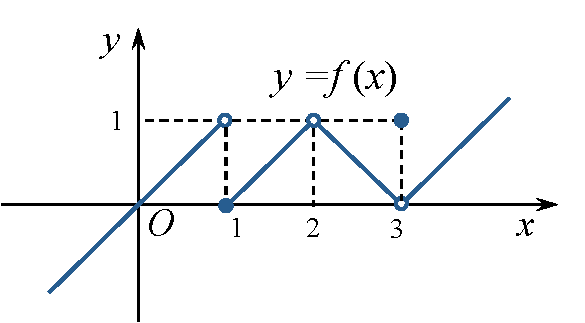
\includegraphics{./images/ch3/limxf.pdf}}
	
	$\limx{1}f(x)$\underline{不存在}
	\quad $\limx{2}f(x)$\underline{$=1$}
	\quad $\limx{1}f(x)$\underline{$=0$}
\end{center}

{\bf 思考:}{\b
	\begin{itemize}
	  \setlength{\itemindent}{1cm}
	  \item 为什么在定义中要求$0<|x-x_0|<\delta$,而不是$|x-x_0|<\delta$?
	  
	   \quad ({\it 因为极限表示的自变量趋于改点的过程中(而不是在该电上)函数值的变化趋势,
	   与函数在该点处的取值无关})
	  \item 符号$f(x_0+0),f(x_0-0)$与$f(x_0)$是何关系?
	  
	  \quad ({\it前两者分别表示左、右极限,最后一个是函数值,三者相互无关})
	\end{itemize}
}

{\bf 例:}证明:$\limx{x_0}\sin x=\sin x_0$。

[证]:对任意$\e>0$,令{\b$\delta=\e$},则当$0<|x-x_0|<\delta$时,有
$$|\sin x-\sin x_0|=2\left|\cos\df{x+x_0}2\right|
\left|\sin\df{x-x_0}2\right|\leq|x-x_0|<\delta=\e,$$
由函数极限定义,即证。\hfill $\Box$

{\bf 例:}证明:$\limx{1}x^2=1$。

[证]:对任意$\e>0$,令{\b$\delta=\min\left\{\df12,\e\right\}$},
\ps{令$\delta\leq\df12$,作用在于使得$|x+1|$有界}
则当$0<|x-1|<\delta$时,有
$$|x^2-1|=|(x+1)(x-1)|<\df32\cdot\delta<\df32\e,$$
由函数极限定义,即证。\hfill $\Box$

{\bf 例:}设$\limx{x_0}f(x)=A$,用定义证明:$\limx{x_0}[f(x)]^3=A^3$

[证]:对任意$\e>0$,由$\limx{x_0}f(x)=A$,存在$\delta>0$,对任意
$0<|x-x_0|<\delta$,有
$$|f(x)-A|<\e.$$
不妨设$\e<1$,由上式可知$0<|x-x_0|<\delta$时,有$|f(x)|<|A|+1$。

综上,记$C=(|A|+1)^2+(|A|+1)|A|+A^2$,则当$0<|x-x_0|<\delta$时,总有
\begin{align}
	|f^3(x)-A^3|&=|f(x)-A||f^2(x)+f(x)A+A^2|\notag\\
	&\leq |f(x)-A|[|f^2(x)|+|f(x)||A|+A^2]\notag\\
	&<\e[(|A|+1)^2+(|A|+1)|A|+A^2]=C\e\notag,
\end{align}
有极限的定义,即证。\hfill $\Box$

\begin{shaded}
	{\bf 【函数极限的反面说法】}
	
	\begin{itemize}
	  \item {\it 当$x\to x_0$时$f(x)$不以$A$为极限:} 
	    $\exists\e_0>0,\forall\delta>0, \exists x^*\in
	    U_0(x_0,\delta),|f(x^*)-A|\geq\e_0$ 
	  \item {\it 当$x\to x_0$时$f(x)$无极限:}
		$\forall A\in\mathbb{R},\exists\e_0>0,\forall\delta>0, \exists x^*\in
	    U_0(x_0,\delta),|f(x^*)-A|\geq\e_0$ 
	\end{itemize}
	
	{\bf 例:}证明:Dirichlet函数在任意点处无极限。
	
	[证]:任取$x_0,A\in\mathbb{R}$,不妨设$A\ne 0$($A\ne 1$的情况同理可证)。
	
	令$\e_0=\df{|A|}2$,对任意$\delta>0$,由有理数的稠密性,总可以在
	$U_0(x_0,\delta)$内取得某个有理数$x^*$,从而$D(x^*)=0$,于是
	$$|D(x^*)-A|=|A|>\e_0,$$
	由上述的定义,可知当$x\to x_0$时$D(x)$无极限,又由$x_0$的任意性,可知
	$D(x)$处处无极限。\hfill $\Box$
\end{shaded}

\subsection{函数极限的基本性质}

参考数列极限的性质,可以类似地证明函数极限的下列性质。

{\bf 唯一性:}函数极限若存在,必唯一。

{\bf 有界性:}
\begin{enumerate}[(1)]
  \setlength{\itemindent}{1cm}
  \item 若$\limx{+\infty}f(x)=A$,则$f(x)$当$x$充分大时有界
  \ps{当$x$充分大时,等价于,存在$X$,当$x>X$时}
  \item 若$\limx{x_0}f(x)=A$,则$f(x)$当$x$充分靠近$x_0$时有界
  \ps{当$x$充分靠近$x_0$时,等价于,存在$\delta>0$,
  当$x\in U_0(x_0,\delta)$时}
\end{enumerate}

{\bf 注意:}函数极限有界性和数列极限有界性的叙述存在的差异:
{\it\b 数列收敛则数列整体有界\ps{数列极限中的数列整体都有界,
是由数列自身的“稀疏”特性所决定的},
函数收敛只能说明在趋近的过程中(或者充分靠近目标时)有界!}请思考一下这是为什么?

[提示]:极限$\limx{+\infty}\df1x=0$,但$\df1x$在定义域上无界;
类似地,$\limx{1}x=1$,但$x$显然也是无界的。

{\bf 保号性:}
\begin{enumerate}[(1)]
  \setlength{\itemindent}{1cm}
  \item 若$\limx{+\infty}f(x)=A>0$,则当$x$充分大时,$f(x)>0$
  \item 若$\limx{x_0}f(x)=A>0$,则当$x$充分靠近时$x_0$时,$f(x)>0$
\end{enumerate}

{\bf 函数极限与数列极限的关系:}({\it Henie定理})
\ps{Henie(1821-1881),德国数学大师Weierstrass的学生。-
1872年证明:有界闭区间上的连续函数必是一致连续的。也即,如果把函数的定义限定在闭区间上,
连续和一致连续的差别将随之消失。} 
已知$\limx{x_0}f(x)=A$,若若数列$\{x_n\}$取值在$f(x)$的定义域内,
且满足:$x_n\to x_0(n\to$ $\infty)$,$x_n\ne 0\;(n\in\mathbb{Z}_+)$,
则必有$\limn f(x_n)=A$。

[证]:已知$\limx{x_0}f(x)=A$,故对任意$\e>0$,存在$\delta>0$,
使对任意$x\in U_0(x_0,\delta)$,都有$|f(x)-A|<\e$。

设$\limn x_n=x_0$,则以上的$\delta>0$,存在$N\in\mathbb{Z}_+$,
使对任意$n>N$,都有$|x_n-x_0|<\delta$。从而,当$n>N$时,必有
$$|f(x_n)-A|<\e.$$
即证。\hfill $\Box$

对于$x\to x_0^+$和$x\to x_0^-$的情形,该定理显然也成立。

与上一节子数列有关收敛性质的用途一样,Henie定理的用途更多地是证明函数极限不存在。
当然,有时遇到一些不方便计算的数列极限,将其转化为对应的函数极限来计算
\ps{由于计算函数极限有类似L'Hospital法则和Taylor公式这样的工具,相对来说
比计算数列极限方法更多样}。

{\bf 例:}{\b 证明:$f(x)=\sin\df 1x$当$x\to 0$时无极限。}\ps{KD教材3.2.2节-例8}

[证]:令
$$x^{(1)}_n=\df1{n\pi},\quad
x^{(2)}_n=\df1{2n\pi+\df{\pi}2},\quad n\in\mathbb{Z}_+$$ 
显然,$\limn x^{(1)}_n=\limn x^{(2)}_n=0$,且
$$f(x^{(1)}_n)\equiv0,\quad f(x^{(2)}_n)\equiv1,$$
进而
$$\limn f(x^{(1)}_n)=0\ne1=\limn f(x^{(2)}_n),$$
由Henie定理,即知极限不存在。\hfill $\Box$

\begin{center}
	\resizebox{!}{5cm}{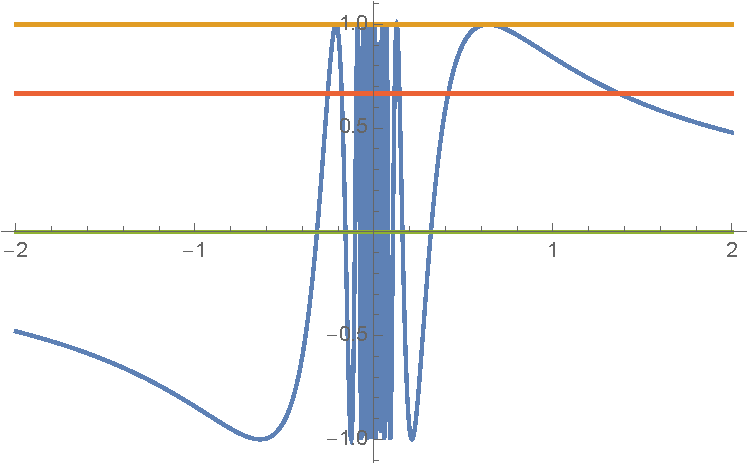
\includegraphics{./images/ch3/sin1x.pdf}}
	
	{\it 以上所取的$x^{(1)}_n$和$x^{(2)}_n$分别取自图上绿色和黄色水平线与
	函数$\sin\df1x$的交点,事实上,对于任意的$a\in[-1,1]$(红色水平线),
	都可以取得类似的点列,用于构造证明所需的收敛到不同值得函数值数列,请思考以下如何写
	出其表达式?
	$$x^{(a)}_n=\df1{2n\pi+\arcsin a},\quad n\in\mathbb{Z}_+$$}
\end{center}

% \begin{shaded}
	{\bf 例:}用Henie定理证明Dirichlet函数在任意点处无极限。
	
% 	{\bf 命题:}对任意$x_0\in\mathbb{R}$,都存在这样的两个数列
% 	$\{x_n^{(1)}\}$和$\{x_n^{(2)}\}$,满足
% 	$$x_n^{(1)}\in\mathbb{Q},\;x_n^{(2)}\notin\mathbb{Q}\;(n\in\mathbb{Z}_+),$$
% 	且
% 	$$\limn x_n^{(1)}=\limn x_n^{(2)}=x_0.$$
% 	
% 	{\bf 思考:}试给出$\{x_n^{(1)}\}$和$\{x_n^{(2)}\}$的通项表达式。
	
	[证]:
% 	1)若$x_0\in\mathbb{Q}$,可令
% 	$$x_n^{(1)}=x_0+\df1n,\quad
% 	x_n^{(2)}=x_0+\df{\sqrt2}n,\;(n\in\mathbb{Z}_+)$$
% 	2)若$x_0\notin\mathbb{Q}$,可令
% 	$$x_n^{(1)}=[x_0]+x_0\mbox{\it 小数部分的前}n\mbox{\it 位},
% 	\;(n\in\mathbb{Z}_+)$$
% 	例如$x_0=\pi=3.1415926\ldots$,则
% 	$$x_1^{(1)}=3.1,\;x_2^{(1)}=3.14,\;x_3^{(1)}=3.141,\;
% 	x_4^{(1)}=3.1415,\;\ldots$$
% 	另,
% 	$$x_n^{(2)}=x_0+\df1n,\;(n\in\mathbb{Z}_+)$$
% 	
% 	{\bf 又解:}
	对任意$x_0$,定义
	$$x_n=[x_0]+x_0\mbox{\it 小数部分的前}n\mbox{\it 位},$$
	$$x_n^{(1)}=x_n+\df1n,$$
	$$x_n^{(2)}=x_n+\df{\sqrt2}n,$$
	显然$\{x_n^{(1)}\}$和$\{x_n^{(2)}\}$分别为趋于$x_0$的有理和无理数列,而
	$$\limn D(x_n^{(1)})=1\ne0=\limn D(x_n^{(2)}),$$
	从而由Hiene定理,即证。\hfill $\Box$
% \end{shaded}

{\bf 例:}设在$(0,+\infty)$上,恒有$f(x^2)=f(x)$,且
$$\limx{0^+}f(x)=\limx{+\infty}f(x)=f(1)$$
证明:$f(x)=f(1)\,(x\in(0,+\infty))$

[提示]:对任意$x_0>1$,都有
$$f(x_0)=f(x_0^2)=f(x_0^4)=\ldots=\limn f(x_0^{2^n})=\limx{+\infty}f(x)=f(1).$$
对任意$x_0<1$,都有
$$f(x_0)=f(x_0^2)=f(x_0^4)=\ldots=\limn f(x_0^{2^n})=\limx{0^+}f(x)=f(1).$$

\section{无穷小与无穷大}

\subsection{无穷小}

以下$\Delta$表示$x_0,x_0^+,x_0^-,\infty,+\infty,-\infty$中的任意一个。

若$\limx{\Delta}f(x)=0$,则称{\it $f(x)$为$x\to\Delta$时的无穷小},记为
$${\b f(x)=\circ(1),\;(x\to\Delta).}$$

注意,{\b 谈到无穷小,一定是和某个变化过程相对应的}。例如:$f(x)=x-1$是$x\to 1$时的
无穷小,但不是$x\to 2$时的无穷小。

显然,常值函数$f(x)\equiv 0$是任何过程中的无穷小。

利用函数极限和无穷小的定义,容易证明:
$\limx{\Delta}f(x)=A\Leftrightarrow f(x)=A+\alpha$,其中$\alpha$
  是$x\to\Delta$时的无穷小。
% \begin{enumerate}[(1)]
%   \setlength{\itemindent}{1cm}
%   \item 
%   \item $\limx{\Delta}f(x)=A$,$\alpha$是$x\to\Delta$时的无穷小,则$\alpha f(x)$
%   也是$x\to\Delta$时的无穷小,也即:{\it 在同一过程中,无穷小和有界函数的乘积仍为无穷小}。
% \end{enumerate}

\subsection{无穷大}

无穷大意味着在某个过程中,函数的绝对值会无限增大,这同时也就意味着其倒数会趋于零。

若$\limx{\Delta}\df1{f(x)}=0$,则称{\it $f(x)$为$x\to\Delta$时的无穷大}。
\ps{这里我们的定义和同济的教材上略有区别,但是完全等价}。

需要注意的是,无穷大和无界是不同的。例如:$f(x)=x$和$g(x)=x\sin x$都是$x\to\infty$时
的无界量(即:只要$x$充分远离原点,则函数值可以超过任何事先给定的值),但前者是该过程中的
无穷大,后者不是。

此外,{\b 要注意无穷大有正负之分,而无穷小没有。}

无穷大的等价定义:$f(x)$为$x\to\Delta$时的无穷大,也即:
对于任意$M>0$,当$x$充分靠近$\Delta$时,总有$|f(x)|>M$。
下面就$x\to x_0$的情况给出证明。

{\bf 例:}证明:$f(x)$为$x\to x_0$时的无穷大,也即:
对于任意$M>0$,存在$\delta>0$,使对任意$x\in U_0(x_0,\delta)$,总有$|f(x)|>M$。

[证]:任取$M>0$,令$\e=\df1M$。由无穷大的定义,$\limx{\Delta}\df1{f(x)}=0$,故对
此$\e$,存在$\delta>0$,使对任意$x\in U_0(x_0,\delta)$,总有
$$\left|\df1{f(x)}\right|<\e\quad\Rightarrow |f(x)|>\df1{\e}=M.$$
即证。\hfill $\Box$

{\b$x\to x_0$或$x_0^+,x_0^-$时的无穷大对应的是函数曲线的{\it 铅直渐近线}}。例如:
$\limx{0}\df1x=0$,故$x=0$是$f(x)=\df1x$的铅直渐近线;
$\limx{\pi/2^+}\tan x=-\infty$,故$x=\pi/2$是$f(x)=\tan x$的铅直渐近线。

{\bf 补充例题:}

{\bf 例:}设当$x\to
x_0$时,$f(x)$不是无穷大,则下列命题中正确的是(D)
\begin{enumerate}[(A)]
  \setlength{\itemindent}{1cm}
  \item 若$g(x)$是$x\to x_0$时的无穷小,则$f(x)g(x)$必为$x\to x_0$时的无穷小
  \item 若$g(x)$不是$x\to x_0$时的无穷小,则$f(x)g(x)$必不是$x\to x_0$时的无穷小
  \item 若$g(x)$在$x_0$的某邻域内无界,则$f(x)g(x)$必为$x\to x_0$时的无穷大
  \item 若$g(x)$在$x_0$的某邻域内有界,则$f(x)g(x)$必不是$x\to x_0$时的无穷大
\end{enumerate}

\section{极限运算法则}

以下讨论的所有性质都是指在同一个$x\to\Delta$的极限过程中。

\subsection{极限的四则运算}

{\bf 定理:}
\begin{enumerate}[(1)]
  \setlength{\itemindent}{1cm}
  \item 有限个无穷小的和也是无穷小;
  \item 有界函数与无穷小的乘积是无穷小;
  \item 有限多个无穷小的乘积是无穷小。
\end{enumerate}

{\bf 推论:}若相关极限都有意义,且符合代数运算的基本条件,则极限运算总可以
和有限多次的四则运算交换次序。

{\bf 以上的结论都可以直接套用于数列的极限。}

如果不是有限次数的四则运算,随意交换极限运算和四则运算的次序,
则可能出现如下的错误:
{\b
\begin{align*}
	1&=\limn1=\limn\left(\underbrace{\df1n+\df1n+\ldots+\df1n}
	_{n\mbox{\footnotesize 个}}\right)\\
	&=\underbrace{\limn\df1n+\limn\df1n+\ldots+\limn\df1n}
	_{n\mbox{\footnotesize 个}}\\
	&=\underbrace{0+0+\ldots+0}_{n\mbox{\footnotesize 个}}=0
\end{align*}
}

相当于$n$落在了极限符号之外,显然错误!!

{\bf 例:}计算极限
$$\limx{\infty}\df{3x^3+2x-1}{4x^3+6x^2+9}$$

[解]:
\begin{align}
	\limx{\infty}&\df{3x^3+2x-1}{4x^3+6x^2+9}
	=\limx{\infty}\df{3+2\frac1{x^2}-\frac1{x^3}}
	{4+6\frac1x+9\frac1{x^3}}
	=\df{\limx{\infty}\left(3+2\frac1{x^2}-\frac1{x^3}\right)}
	{\limx{\infty}\left(4+6\frac1x+9\frac1{x^3}\right)}\notag\\
	&=\df{\limx{\infty}3+\limx{\infty}2\frac1{x^2}-\limx{\infty}\frac1{x^3}}
	{\limx{\infty}4+\limx{\infty}6\frac1x+\limx{\infty}9\frac1{x^3}}
	=\df{\limx{\infty}3+\limx{\infty}2\limx{\infty}\frac1{x^2}
	-\limx{\infty}\frac1{x^3}}
	{\limx{\infty}4+\limx{\infty}6\limx{\infty}\frac1x
	+\limx{\infty}9\limx{\infty}\frac1{x^3}}\notag\\
	&=\df{3+2\cdot 0-0}{4+6\cdot 0+9\cdot 0}=\df34\notag
\end{align}
\hfill $\Box$

在日常的解题中,计算过程显然不必都如此详细。

对于与该例类似的极限问题,我们有如下的结论,在今后的极限计算中可以直接应用:

{\b 设$P(x)$和$Q(x)$分别为$m$和$n$次多项式函数,且其最高次项系数分别为
$a,b$,$ab\ne 0$,则
$$
	\limx{+\infty}\df{P(x)}{Q(x)}=
	\left\{\begin{array}{ll}
		a/b, & m=n;\\
		0, & m<n;\\
		\mbox{不存在}, & m>n.
	\end{array}\right.
$$
}

{\bf 定理:}{\b 初等函数运算可以和极限运算交换次序}
\ps{后续章节中,我们将学习到因为初等函数在其定义区间内均连续,故初等函数运算可以和
极限运算交换次序}

{\bf 补充例题:}

{\bf 例:}判断与分析
\begin{enumerate}[(1)]
  \setlength{\itemindent}{1cm}
  \item 若$x\to x_0$时,$f(x)$有极限,$g(x)$无极限,则当$x\to x_0$时,以下哪些函数必无极限:
  $$f(x)g(x),\quad [g(x)]^2,\df{g(x)}{f(x)}, f(x)+g(x)$$ 
  \item 若$\limx{x_0}g(x)=A,\lim\limits_{u\to A}f(u)=B$,是否必有
  $\limx{x_0}f[g(x)]=B$?
  \item 若$\limx{x_0}f(x)g(x)=0$,则当$x\to
  x_0$时, $f(x),$ $g(x)$之一必趋于$0$ ({$\times$})
\end{enumerate}

{\bf 例:}计算极限
$$\limn\df{\cos^n\theta-\sin^n\theta}{\cos^n\theta+\sin^n\theta}\quad
(0\leq\theta\leq\df{\pi}{2})$$

[提示]:根据$\theta$的取值范围,决定是分子分母同时除以$\sin^nx$还是$\cos^nx$,结果
$$\mbox{原式}=\left\{\begin{array}{ll}
-1,& 0<\theta<\df{\pi}4\\
0,& \theta=\df{\pi}4\\
1,& \df{\pi}4<\theta<\df{\pi}2
\end{array}\right.$$

{\bf 例:}$|x|<1$,计算
$$\limn(1+x)(1+x^2)\ldots(1+x^{2^n})$$

[提示]:
$$(1+x)(1+x^2)\ldots(1+x^{2^n})=\df{(1-x)(1+x)(1+x^2)\ldots(1+x^{2^n})}{1-x}
=\df{1-x^{2^{n+1}}}{1-x}$$

{\bf 例:}$|\lambda|<1$,计算$\limn(\lambda+2\lambda^2+\ldots+n\lambda^n)
 =\df{\lambda}{(1-\lambda)^2}$ \hfill({\it 等比数列求和})

{\bf 例:} $\limn\left(\sqrt{n+3\sqrt n}-\sqrt{n-\sqrt{n}}\right)=2$
\hfill({\it 分子有理化})

{\bf 例:} $\limn\left(\sqrt[3]{n^3+2n^2+1}-n\right)=\df23$
% \ps{$a^n-b^n=(a-b)(a^{n-1}+a^{n-2}b+\ldots+b^{n-1})$}
\hfill({\it 分子有理化})

[提示]:利用公式$a^n-n^n=(a-b)(a^{n-1}+a^{n-2}b+\ldots+b^{n-1})$
进行分子有理化:
$$\mbox{原式}=\limn\df{2n^2+1}{(n^3+2n^2+1)^{\frac23}
+(n^3+2n^2+1)^{\frac13}n+n^2}$$

{\bf 例:} $\limn\left(1-\df1{2^2}\right)\left(1-\df1{3^2}\right)\ldots
\left(1-\df1{n^2}\right)=\df12$\hfill({\it 因式分解,消去公共部分})

{\bf 例:} $\limn\sin^2\left(\pi\sqrt{n^2+n}\right)$\hfill({\it 周期性结合分子有理化})

{\bf 例:} $\limn\df32\cdot\df54\cdots\df{2^n+1}{2^n}
=\limn2\left(1-\df12\right)\left(1+\df12\right)\left(1+\df1{2^2}\right)
\ldots\left(1+\df1{2^n}\right)=2$

{\bf 例:} $\sqrt{n+\sqrt{n+\sqrt n}}-\sqrt n\to\df12,\;(n\to\infty)$
\hfill({\it 分子有理化})

\subsection{复合函数的极限}

设有复合函数$y=f[g(x)]$,其中\ps{对比Henie定理}
$$\limx{x_0}g(x)=u_0,\quad\lim\limits_{u\to u_0}f(u)=A,$$
且在$x_0$附近$g(x)\ne u_0$,则
$$\limx{x_0}f[g(x)]=A.$$

{\bf 注:}{\b 为什么要求“在$x_0$附近$g(x)\ne u_0$”?}
  
  答:因为$f(x)$可能在$x_0$处的定义与极限值无关,例如:
  $$f(x)=\left\{\begin{array}{ll}
  1,&x\ne0\\0,&x=0
  \end{array}\right.$$
  $g(x)\equiv 0$,则$f(g(x))\equiv0$,从而$\limx{0}f(g(x))=0$,
  而不是如定理所述$\limx{0}f(g(x))=1$

直观的理解,以上的结论告诉我们:若相关极限都存在,则极限运算可以和函数运算交换次序。

显然,这个结论可以类似地推广到$x\to\infty$的情形。

\section{极限存在准则与两个重要极限}

\subsection{夹逼准则}

有时也叫{\it 迫敛准则}或者{\it 三明治定理}。

{\bf 准则I:}设对任意$n\in\mathbb{N}$,$x_n\le a_n\le y_n$,
且$\{x_n\},\{y_n\}$收敛于相同的极限$a$,则$\limn a_n=a$。

\begin{center}
	\resizebox{!}{5cm}{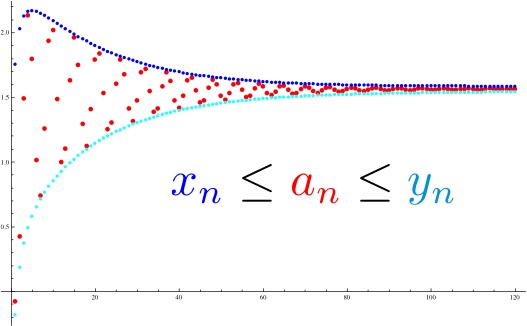
\includegraphics{./images/ch2/xay_n.jpg}}
\end{center}

{\bf 例:}证明:$\limn (\sqrt{n+1}-\sqrt{n})=0$。

[证](夹逼准则):注意到
$$0<\sqrt{n+1}-\sqrt{n}={\b\df1{\sqrt{n+1}+\sqrt{n}}
\leq\df 1{\sqrt{n}}},$$
又
$$\limn 0=\limn\df 1{\sqrt{n}}=0,$$
故由夹逼准则,可知$\limn (\sqrt{n+1}-\sqrt{n})=0$。\hfill $\Box$

对比一下用定义证明的过程:

[证](定义):对任意$\e>0$,令$N=[1/\e^2]+1$,则对任意$n>N$,总有
$$\left|\sqrt{n+1}-\sqrt{n}-0\right|
={\b\df1{\sqrt{n+1}+\sqrt{n}}\leq\df 1{\sqrt{n}}}
<\df 1{\sqrt{N}}<\df 1{\sqrt{1/\e^2}}=\e,$$
由此可知$\limn (\sqrt{n+1}-\sqrt{n})=0$。\hfill $\Box$

不难发现,两个证明中最关键的放缩步骤是完全一致的,而使用夹逼准则时,可以直接
使用一些已知的或“简单的”极限结论,避免了推导$N$的繁琐过程,因此过程显得更加
简洁也更容易理解。

{\bf 思考:}证明:$\limn [(n+1)^k-{n}^k]=0$,其中$0<k<1$。

[提示]:$n^k\left[\left(1+\df1n\right)^k-1\right]
<n^k\left(1+\df1n-1\right)=n^{k-1}\to 0\;(n\to\infty)$

{\bf 例:}\ps{KD教材2.2.3节-例6,重点掌握结论!}
证明:{\b 若$a>0$为常数,则$\limn \sqrt[n]{a}=1$}。

{\bf 例:}计算极限
\begin{enumerate}[(1)]
  \setlength{\itemindent}{1cm}
  \item $\limn\sqrt[n]{n^5}=1$
  \item $\limn\sqrt[n^2]{5^n+1}=1$
  \item 已知$a>b>0$,$\limn\sqrt[n]{\df1{a^n}+\df1{b^n}}=\df1b$
  \item 设$a_k\geq0,\;(k=1,2,\ldots)$,则$\limn\sqrt[n]
  {\sum\limits_{k=1}^na_k^n}=\max\limits_{1\leq k\leq n}a_k$
\end{enumerate}
 
{\bf 补充例题:}

{\bf 例:} $\limn\df{\sqrt{n+\sqrt n}-\sqrt n}{\sqrt[n]{3^n+5^n+7^n}}=\df1{14}$

% {\bf 例:} 已知$\limn a_n=A$,
% \begin{enumerate}[(1)]
%   \setlength{\itemindent}{1cm}
%   \item 证明:$\limn\df{[na_n]}n=A$
%   \item 若$\lambda\in(0,1)$,计算:
%   $$\limn(a_n+\lambda a_{n-1}+\lambda^2a_{n-2}+\ldots+\lambda^na_0)=\df
%   A{1-\lambda}$$
% \end{enumerate}

{\bf 例:} $\limn\sqrt[n]{n^5+5^n}=5$

{\bf 例:} 设$x\geq 0$,则
$\limn\sqrt[n]{1+x^n+\left(\df{x^2}2\right)^n}=
\left\{\begin{array}{ll}
1&x\in[0,1]\\ x & x\in(1,2]\\ \frac{x^2}2& x>2
\end{array}\right.$

{\bf 例:} $\limn\left(\df1{n+1}+\df1{\sqrt{n^2+1}}+\ldots
+\df1{\sqrt[n]{n^n+1}}\right)=1$

{\bf 例:}已知$k\in\mathbb{Z}_+$,计算:$\limn n^2\left(\df kn-\df1{n+1}-\df1{n+2}
-\ldots-\df1{n+k}\right)$

[提示]:
$$\df kn-\df1{n+1}-\df1{n+2}-\ldots-\df1{n+k}=\sum\limits_{i=1}^k\df{i}{n+i}$$
$$\df i{n(n+k)}\leq\df{i}{n+i}\leq\df i{n(n+1)}$$

{\bf 准则I':}设在$x_0$的某邻域内,恒有
$$\varphi(x)\leq f(x)\leq\psi(x), $$
且$\limx{x_0}\varphi(x)=\limx{x_0}\psi(x)=A$,则
$$\limx{x_0}f(x)=A.$$

{\bf 注:}该准则显然可以推广到$x$趋于无穷的情形。

{\bf 例:}\ps{KD教材3.2.3节-例11}(重要极限)证明:
$$\b\limx{0}\df {\sin x}x=1$$

[提示]:
\begin{center}
	\resizebox{!}{5cm}{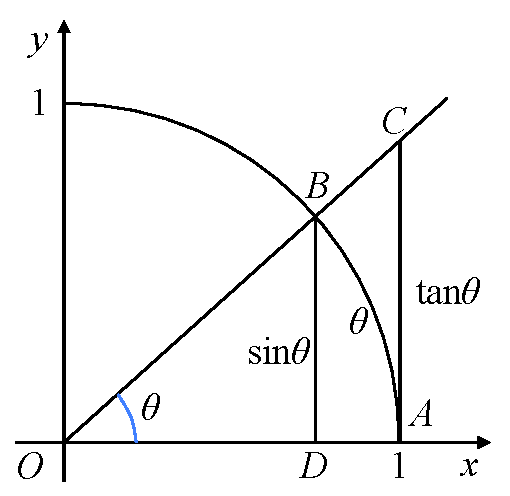
\includegraphics{./images/ch3/xsintan.pdf}}
\end{center}

如图,显然弧$AB$的长度大于直线$BD$,即$\sin\theta<\theta$;又扇形$ABO$的面积
$\df12\theta$小于三角形$ACO$的面积$\df12\tan\theta$,从而$\theta<\tan\theta$

{\b
{\bf 例:}从重要极限$\limx{0}\df{\sin x}x=1$出发可得到的一些常用的极限
\begin{enumerate}[(1)]
  \setlength{\itemindent}{1cm}
  \item $\limx{0}\df{\sin\sin x}{\sin x}=1$ 
  \item $\limx 0\df{1-\cos x}{x^2}=\df12$ 
  \item $\limx 0\df{\sin mx}{\sin nx}=\df mn$
  \item $\limx 0\df{\tan x}{x}=1$
  \item $\limx 0\df{\arcsin x}x=1$
  \item $\limx 0\df{\arctan x}x=1$
  \item $\limx a\df{\sin x-\sin a}{x-a}=\cos a$
\end{enumerate}
}

{\bf 例:}设$f(x)=\sum\limits_{i=1}^na_i\sin
ix$,其中$a_i(i=1,2,\ldots,n)$为常数,且对任意$x\in\mathbb{R}$, $|f(x)|\leq |\sin x|$,证明:
$$\left|a_1+2a_2+\ldots+na_n\right|\leq 1$$

[提示]:{\b 极限运算可以和绝对值运算交换次序!}

\subsection{单调有界准则(原理)}

{\bf 准则II:}单调有界数列必有极限。

即:若数列{\it 从某一项开始}\ps{为什么是从某一项开始?}
严格单调递增(减),且有上(下)界,则该数列收敛。

[证]:假设$\{a_n\}$单调递增有上界,由确界原理,可知其必有上确界,记为$A$。
以下证明$\limn a_n=A$。

事实上,对任意$\e>0$,由上确界的定义,必存在某个$a_N$,使得
$$A-\e<a_N\leq A.$$

$\{a_n\}$单调递增,故对任意$n>N$,恒有$a_n\geq a_N$,又$a_n\leq A$,从而
$$a_n\leq a_n\leq A\quad\Rightarrow\quad |a_n-A|<\e,$$
由极限的定义,即证。\hfill $\Box$

单调有界原理可以证明极限的存在性(或数列的收敛性),但常常无法给出具体的极限值。
例如下面的重要极限:

{\bf 例:}\ps{KD教材2.2.4节-例7,重点掌握结论}
证明:数列$\left\{\left(1+\df1n\right)^n\right\}$收敛。

该数列的极限通常记为$e$,称为{\kaishu Napier常数}\ps{同济教材称之为Euler常数,
我们沿用的是维基百科和国际上通行的叫法;Napier是公认的计算过程“机械化”的先驱}。

\begin{shaded}

以上结论的证明作为了解即可。

[提示]:证明数列$\left\{\left(1+\df1n\right)^n\right\}$单调递增有上界。

先证有上界:

\begin{align}
	\left(1+\df1n\right)^n&=1+\df n1\cdot\df1n
	+\df{n\cdot(n-1)}{2\cdot1}\cdot\df1{n^2}+\ldots
	+\df{n\cdot(n-1)\ldots3\cdot2}{(n-1)\cdot(n-2)\ldots2\cdot1}\cdot\df1{n^2}\notag\\
	&<1+1+\df1{2\cdot1}+\ldots+\df1{(n-1)\cdot(n-2)\ldots2\cdot1}
	+\df1{n\cdot(n-1)\ldots2\cdot1}\notag\\
	&<1+1+\df12+\ldots+\df1{2^{n-2}}+\df1{2^{n-1}}<3\notag
\end{align}

再证单调性:

\begin{align}
	\left(1+\df1n\right)^n&=1+\df n1\cdot\df1n
	+\df{n\cdot(n-1)}{2\cdot1}\cdot\df1{n^2}+\ldots
	+\df{n\cdot(n-1)\ldots3\cdot2}{(n-1)\cdot(n-2)\ldots2\cdot1}
	\cdot\df1{n^{n-1}}\notag\\
	&\quad +\df{n\cdot(n-1)\ldots2\cdot1}{n\cdot(n-1)\ldots2\cdot1}
	\cdot\df1{n^{n}}\notag\\
	&=1+1+\df1{2\cdot 1}\left(1-\df1n\right)+\df1{3\cdot2\cdot
	1}\left(1-\df1n\right)\cdot\left(1-\df2n\right)+\ldots\notag\\
	&\quad +\df1{(n-1)\cdot(n-2)\ldots\cdot2\cdot
	1}\left(1-\df1n\right)\cdot\left(1-\df2n\right)
	\ldots\left(1-\df{n-2}n\right)\notag\\
	&\quad +\df1{n\cdot (n-1)\ldots\cdot2\cdot
	1}\left(1-\df1n\right)\cdot\left(1-\df2n\right)
	\ldots\left(1-\df{n-1}n\right)\notag\\
	&>1+1+\df1{2\cdot 1}\left(1-\df1{n-1}\right)+\df1{3\cdot2\cdot
	1}\left(1-\df1{n-1}\right)\cdot\left(1-\df2{n-1}\right)+\ldots\notag\\
	&\quad +\df1{(n-1)\cdot(n-2)\ldots\cdot2\cdot
	1}\left(1-\df1{n-1}\right)\cdot\left(1-\df2{n-1}\right)
	\ldots\left(1-\df{n-2}{n-1}\right)\notag\\
	&=\left(1+\df1{n-1}\right)^{n-1}\notag
\end{align}

关于单调性,也可以用平均值不等式来证明:
$$\left(1+\df1n\right)^n\cdot 1<
\left[\df{n\left(1+\frac1n\right)+1}{n+1}\right]^{n+1}
=\left(1+\df1{n+1}\right)^{n+1}.$$

\end{shaded}

{\bf 注:}需要掌握的重要性质{\b
\begin{itemize}
  \setlength{\itemindent}{1cm}
  \item 数列$\left\{\left(1+\df 1n\right)^n\right\}$严格单调递增有上界;
  \item 数列$\left\{\left(1+\df 1n\right)^{n+1}\right\}$严格单调递减有下界;
  \item 显然,二者极限相同,都为$e$;
  \item 重要不等式:
\end{itemize}}
$$\b\left(1+\df1n\right)^n<e<\left(1+\df1n\right)^{n+1}$$

{\bf 注意:}
{\b 典型错误
\begin{eqnarray*}
	\limn\left(1+\df1n\right)^n&
	=&\limn \underbrace{\left(1+\df 1n\right)\left(1+\df 1n\right)\cdots
	\left(1+\df	1n\right)}_{n\mbox{\footnotesize\it 个}}\\
	&=&\underbrace{\limn\left(1+\df1n\right)\limn\left(1+\df1n\right)
	\cdots\limn\left(1+\df1n\right)}_{n\mbox{\footnotesize\it个}}\\
	&=&\left[\limn\left(1+\df1n\right)\right]^n=1
\end{eqnarray*}}

相当于$n$落在了极限符号之外,显然错误!!此外,不要忘记,极限运算应该和有限次的四则
运算交换次序。


\begin{shaded}
	{\bf 关于Napier常数$e$}
	
	{\bf 例:}若将$a>0$分成若干份,使得总乘积最大,由平均值不等式可知,显然
	等分最有利,但该分成多大的一份呢?分析可证明分成最接近于$e$的大小最合适。
	
	{\bf 例:}$\e_n=e-\sum\limits_{k=0}^n\df1{k!}$,则
	$$\limn\e_n(n+1)!=1$$
	
	[提示]:利用$\df00$型的Stolz定理(关于该定理参见第三章关于L'Hospital法则的介绍)。
	
	{\bf 例:}$\delta_n=e-\left(1+\df1n\right)^n
	<\left(1+\df1n\right)^{n+1}-\left(1+\df1n\right)^n
	=\left(1+\df1n\right)^n\df1n<\df en<\df3n$
	
	事实上,$\limn\df{2n\delta_n}e=1$
	
	{\bf 重要不等式:}由{$\left(1+\df1n\right)^n<e<\left(1+\df1n\right)^{n+1}$},
	可得
	$${\b \df1{n+1}<\ln\left(1+\df1n\right)<\df1n}$$

	{\bf 例:}证明$a_n=\df1{n+1}+\ldots+\df1{2n},\;(n\in\mathbb{Z}_+)$收敛。

	[提示]:利用$\df1{n+1}<\ln\left(1+\df1n\right)<\df1n$,极限为$\ln2$

	{\bf Euler常数:}
	$$\gamma=\limn\left(\sumn\df1k-\ln n\right)\approx 0.5772\ldots$$
\end{shaded}

利用前述的一些性质,结合夹逼准则,我们可以推广以上的极限得到{\it 第二个重要极限}:
$$\b\limx{\infty}\left(1+\df1x\right)^x=e.$$

[证]:先证明$\limx{+\infty}\left(1+\df1x\right)^x=e$。

以下$[x]$表示对$x$下取整。

对任意$x>0$,显然$[x]\leq x<[x]+1$,于是由前述的重要不等式
$$\left(1+\df1n\right)^n<e<\left(1+\df1n\right)^{n+1},$$
可得
$$\left(1+\df1{[x]+1}\right)^{[x]}<\left(1+\df1x\right)^x
<\left(1+\df1{[x]}\right)^{[x]+1}.$$
利用前述极限容易证明以上不等式两边的数列极限均为$e$,从而由夹逼准则,
$\limx{+\infty}\left(1+\df1x\right)^x=e$。

下证$\limx{-\infty}\left(1+\df1x\right)^x=e$。

事实上,记$y=-x$,则
\begin{align*}
	\limx{-\infty}\left(1+\df1x\right)^x
	&=\lim\limits_{y\to+\infty}\left(1-\df1y\right)^{-y}
	=\lim\limits_{y\to+\infty}\df1{\left(1-\df1y\right)^{y}}\\
	&=\lim\limits_{y\to+\infty}\left(\df y{y-1}\right)^{y}
	=\lim\limits_{y\to+\infty}\left(1+\df1{y-1}\right)^{y}\\
	&=\lim\limits_{y\to+\infty}\left(1+\df1{y-1}\right)^{y-1}
	\lim\limits_{y\to+\infty}\left(1+\df1{y-1}\right)=e\cdot1=e
\end{align*}
\hfill $\Box$

\begin{shaded}
另一种证明思路:
令$f_u(x)=x^ue^{-x}(x\geq 0)$,对于确定的$u$,证明:
\begin{enumerate}[(1)]
  \setlength{\itemindent}{1cm}
  \item $f_u(x)$在$x=u$处取最大值;
  \item 由$f_u(x)>f_u(u+1)$和$f_{u+1}(u+1)>f_u(u)$推出
  $$\left(\df{u+1}u\right)^u<e<\left(\df{u+1}u\right)^{u+1}$$
  \item $\df u{u+1}e<\left(\df{u+1}u\right)^u<e$,由此推出
  $$\lim\limits_{u\to+\infty}\left(1+\df 1u\right)^u=e$$
\end{enumerate}
\hfill $\Box$
\end{shaded}

{\b{\bf 例:}从重要极限$\limx{\infty}\left(1+\df1x\right)^x=e$
出发可得到的一些常用的极限
\begin{enumerate}[(1)]
  \setlength{\itemindent}{1cm}
  \item $\limx{0}(1+x)^{1/x}=1$ 
  \item $\limx 0(1+\sin x)^{1/\sin x}=1$ 
  \item $\limx 0\df{\ln(1+ax)}{x}=a$
  \item $\limx 0\df{e^{ax}-1}{x}=a$ 
  \item $\limx 0\df{a^x-1}{x}=\ln a$ 
  \item $\limx 0\df{(1+x)^a-1}x=a$
  \item $\limn n(\sqrt[n]{a}-1)=\ln a$ 
\end{enumerate}}

单调有界准则一个很常见的应用领域时判断递推数列的敛散性。

{\bf 例:}\ps{KD教材2.2.5节-例9}
设$a_1>0$,$a_{n+1}=\df 12\left(a_n+\df 1{a_n}\right)\,
(n=1,2,\ldots)$,证明$\{a_n\}$收敛,并求其极限。

{\bf 例:}证明极限存在,然后求出极限的值
\begin{enumerate}[(1)]
  \setlength{\itemindent}{1cm}
  \item $\limn\df{n^2}{a^n}\quad (a>1)$%\hfill({\it 单调递减有下界,极限为$0$})
  \ps{\b 由(1)可推广得到一个常用的结论:$b>0,|a|<1$,则$n^ba^n\to 0$}
  \item $\limn\df{n!}{n^n}$%\hfill({\it 单调递减有下界,极限为$0$})
%   \item 设$c>0$,求$\limn\underbrace{\sqrt{c
%   +\sqrt{c+\ldots+\sqrt{c}}}}_{n\mbox{\small 个根号}}$
\end{enumerate}

[解]:(1)\;记$b_n=\df{n^2}{a^n}$,则
$$b_{n+1}=\df{(n+1)^2}{n^2a}b_n,$$
注意到$\limn\df{b_{n+1}}{b_n}=\df1a<1$,故当$n$充分大时,$\{b_n\}$严格单调递减,
而显然$b_n>0$,故由单调有界原理,$\{b_n\}$收敛,设其极限为$A$。在前述递推式两端同时取极限,
可得
$$A=\df1aA\quad\Rightarrow\quad A=0,$$
即为所求。

(2)\;类似解法,略。\hfill $\Box$

{\bf 注:}{\b 若极限存在,可由通项公式反推递推式,然后两边取极限,解方程求得极限值}

{\bf 补充例题:}

{\bf 例:}$x_1=\df c2$,$x_{n+1}=\df c2+\df{x_n^2}2\,(n\in\mathbb{Z}_+)$,
证明:若$c>1$,则$\{x_n\}$发散。

[提示]:设极限为$A$,则$A^2-2A+c=0$,$c>1$时,无解,必发散。

{\bf 例:}$a_0>b_0>0$,
$$a_n=\df12(a_{n-1}+b_{n-1}),\quad
b_n=\sqrt{a_{n-1}b_{n-1}}\;(n\in\mathbb{Z}_+)$$
证明:$\{a_n\},\{b_n\}$收敛于同一极限。

[提示]:$b_0<b_1<a_1<a_0$,利用数学归纳法证明:
$$b_0<b_1<\ldots<b_n<a_n<\ldots<a_1<a_0$$

{\bf 例:}证明:$a_n=\sqrt{1+\sqrt{2+\ldots+\sqrt{n}}}$收敛。

[提示]:注意到
$$\sqrt{n-1+\sqrt n}<\sqrt{n-1+2\sqrt{n-1}+1}=\sqrt{n-1}+1,$$
然后利用不等式$\sqrt{n-1}<2\sqrt{n-2}$递推。

{\bf 例:}给定$x\in(0,3),\; x_{n+1}=\sqrt{x_n(3-x_n)},\;(n\in\mathbb{Z}_+)$,
证明数列$\{x_n\}$收敛,并求其极限。

[提示]:$0<x_2\leq\df12[x_1+(3-x_1)]=\df32$,递推可得
$0<x_n\leq\df32$。另一方面,
$$x_{n+1}-x_n=\df{\sqrt{x_n}(3-2x_n)}{\sqrt{x_n(3-x_n)}+\sqrt{x_n}}\geq 0.$$
即$\{x_n\}$单调递增有上界。

{\bf 例:}证明数列$\{x_n\}:x_1=1,\;x_{n+1}=\df1{1+x_n}$收敛,求其极限。

[提示]:由递推式易得极限$a=\df{\sqrt5-1}2$。(写成:$a$为满足方程$a=\df1{1+a}$的正数)

显然$0<x_n\leq1$,进而$\df1{1+x_n}\geq\df12$。于是\ps{$\{x_n\}$不单调!}
\begin{align}
	|x_{n+1}-a|&=\left|\df1{1+x_n}-\df1{1+a}\right|=\df{|x_n-a|}{(1+x_n)(1+a)}\notag\\
	&<\df{|x_n-a|}{(1+1/2)(1+1/2)}=\df49|x_n-a|\notag\\
	&<\left(\df49\right)^2|x_{n-1}-a|<\ldots<\left(\df49\right)^{n}|x_1-a|,\notag
\end{align}
由夹逼定理可知$|x_{n+1}-a|\to0\;(n\to\infty)$,即证。

% \begin{shaded}
% 	{\bf 特征根法求解求解二阶常系数齐次递推}
% 	
% 	{\bf 例:}已知$a_1,a_2$为常数,数列$\{a_n\}$满足:
% 	$$a_n=\df 12({a_{n-1}+a_{n-2}})\quad(n>2).$$
% 	证明$\{a_n\}$收敛,并求其极限。\ps{\b 熟练掌握此类递推!!!}
% 	
% 	{\bf 解:}原递推式可改写为
% 	$$a_n-a_{n-1}=-\df12(a_{n-1}-a_{n-2})\quad(n>2),$$
% 	由此递推,易得
% 	$$a_n-a_{n-1}=\left(-\df12\right)^{n-2}(a_2-a_1),$$
% 	进而
% 	\begin{align}
% 		a_n&=a_{n-1}+\left(-\df12\right)^{n-2}(a_2-a_1)\notag\\
% 		&=a_{n-2}+\left[\left(-\df12\right)^{n-3}+\left(-\df12\right)^{n-2}\right]
% 		(a_2-a_1)\notag\\
% 		&=\ldots\notag\\
% 		&=a_2+\left[\left(-\df12\right)+\ldots+\left(-\df12\right)^{n-3}
% 		+\left(-\df12\right)^{n-2}\right](a_2-a_1)\notag\\
% 		&=a_2-\df12\df{1-\left(-\df12\right)^{n-2}}{1+\df12}(a_2-a_1)\notag\\
% 		&\to\df13a_1+\df23a_2\;(n\to\infty)\notag
% 	\end{align}
% 	即证。
% 	
% 	{\bf 注:}中学阶段,有些同学接触过所谓的特征根法求递推公式,具体过程如下,其背后
% 	的原理与上面一个例子中的方法是完全一致的。
% 	
% 	已知$a_1,a_2$和如下的递推式:
% 	
% 	$$a_{n+2}=Aa_{n+1}+Ba_n\quad (AB\ne 0, A+B\ne 1),$$
% 	求$\{a_n\}$的通项公式。
% 	
% 	考虑特征方程:
% 	$$r^2=Ar+B$$
% 	\begin{enumerate}[(1)]
% 	  \setlength{\itemindent}{1cm}
% 	  \item 若特征方程有相异实根$p,q$,则
% 	  $$a_n=C_1p^n+C_2q^n$$
% 	  其中系数$C_1,C_2$由方程
% 	  $$\left\{\begin{array}{l}
% 	  a_1=C_1p+C_2q\\
% 	  a_2=C_1p^2+C_2q^2
% 	  \end{array}\right.$$
% 	  可解得
% 	  $$C_1=\df{a_1q-a_2}{p(q-p)},\quad 
% 	  C_2=\df{a_1p-a_2}{q(p-q)}$$
% 	  \item 若有两个相等的实根$r$,则
% 	  $$a_n=[C_1r+C_2(n-1)]r^{n-1}$$
% 	  与(1)类似地可求出系数$C_1,C_2$
% 	\end{enumerate}
% 	
% 	{\bf 例:}Fibonacci数列:$a_{n+2}=a_n+a_{n+1},\;a_1=a_2=1$
% 	
% 	$$a_n=\df1{\sqrt5}\left[\left(\df{1+\sqrt5}2\right)^n
% 	-\left(\df{1-\sqrt5}2\right)^n\right]$$
% 	
% \end{shaded}

{\bf 小结:}求解递推数列的极限问题,注意以下几点:{\b
\begin{itemize}
  \setlength{\itemindent}{1cm}
  \item 递推式两边同时取极限,解方程求得极限的值,是最便利的计算递推数列极限的方法
  \item 若通过以上方法可以求出极限的值,通常只需证明数列单调有界即可
  \item 若该方法无法求得极限的值,则只能利用递推式推导数列通项,进而证明其收敛并计算极限
\end{itemize}}


{\bf 准则II':}设$f(x)$在某个单调且在某个趋势下有界,则
$f(x)$在该趋势下的极限存在。

例如:若$f(x)$在$x_0$的某个左邻域内单调递增且有上界,则$f(x_0-0)$存在;
若$f(x)$当$x$充分大时单调递减且有下界,则$f(+\infty)$存在。

这个准则虽然完全正确,但我们在实际解题中对它应用得并不多。

\subsection{Cauchy极限存在准则}

以下结论也称为{\it Cauchy审敛原理}:

数列$\{a_n\}$收敛,当且仅当:对任意$\e>0$,存在正整数$N$,使对任意$m,n>N$,总有
$$|a_m-a_n|<\e.$$

Cauchy收敛准则的必要性容易证明,但充分性的证明时相当复杂的,不要求掌握。

{\bf 例:}证明$a_n=1+\df12+\df13+\ldots+\df1n$发散。

这里我们要用到Cauchy审敛准则的反面说法:数列$\{a_n\}$发散,当且仅当:存在$\e_0>0$,
使对任意的正整数$N$,都存在$m_0,n_0>N$,使得
$$|a_{m_0}-a_{n_0}|\geq\e_0.$$

[证]:取$\e_0=\df12$,则对任意的正整数$N$,总可以取$m_0=N,n_0=2N$,则
\begin{align*}
	|a_{m_0}-a_{n_0}|
	&=\df1{N+1}+\df1{N+2}+\ldots+\df1{2N}\\
	&>\underbrace{\df1{2N}+\df1{2N}\ldots+\df1{2N}}
	_{N\mbox{\footnotesize 个}}=\df12=\e_0,
\end{align*}
即证。\hfill $\Box$

\subsection{Stolz定理}

{\bf Stolz定理:}
\ps{Stolz定理类似于函数极限中的L'Hospital法则,例如:
对比$\limn\df{n^2}{e^n}$和$\limx{+\infty}\df{x^2}{e^x}$}
($\df{\bm{\infty}}{\bm{\infty}}$形式) 设数列$\{y_n\}$满足$\limn\df
1{y_n}=0$,且$\{y_n\}$至少从某一项开始保持严格单调递增,
则对任意数列$\{x_n\}$,若$\limn\df{x_n-x_{n-1}}{y_n-y_{n-1}}$存在,则必有
$$\limn\df{x_n}{y_n}=\limn\df{x_n-x_{n-1}}{y_n-y_{n-1}}$$

% {\bf 注:}Stolz定理主要用于计算"$\df{\infty}{\infty}$型"的极限

由Stolz定理也可以很容易地得出{\b{\kaishu Cauchy极限定理}:若$\{a_n\}$收敛,则}
$$\b\limn\df{a_1+a_2+\ldots+a_n}n=\limn a_n$$

{\bf 例:}计算以下极限
\begin{enumerate}[(1)]
  \setlength{\itemindent}{1cm}
  \item $\limn\df{1+\sqrt 2+\sqrt[3]{3}+\ldots+\sqrt[n]{n}}{n}$ 
  \item $\limn\df{1^k+2^k+\ldots+n^k}{n^{k+1}},\quad(k\in\mathbb{N})$ 
  \item $\limn\left(\df{1^k+2^k+\ldots+n^k}{n^{k}}-\df
  n{k+1}\right),\quad(k\in\mathbb{N})$
\end{enumerate}
  
  [提示]:(3)以下$P^{(*)}_k(n)$表示以$n$为变量的$k$次多项式,
  \begin{eqnarray*}
  	\mbox{原式}&=&\limn\df{(k+1)(1^k+2^k+\cdots+n^k)-n^{k+1}}{n^k(k+1)}\\
  	&=&\limn\df{(k+1)(n+1)^k-[(n+1)^{k+1}-n^{k+1}]}{(k+1)[(n+1)^k-n^k]}\\
  	&=&\limn\df{(k+1)[n^k+kn^{k-1}+P_{k-2}^{(1)}(n)]
  	-\left[(n+1)^k+(n+1)^{k-1}n+\cdots+n^k\right]}{(k+1)
  	\left[(n+1)^{k-1}+(n+1)^{k-2}n+\cdots+n^{k-1}\right]}\\
  	&=&\limn\df{(k+1)[n^k+kn^{k-1}+P_{k-2}^{(1)}(n)]-(k+1)n^k
  	-\df{k(k+1)}2n^{k-1}-P_{k-2}^{(2)}(n)}
  	{(k+1)\left[\df{k(k+1)}{2}n^{k-1}+P_{k-2}^{(3)}(n)\right]}\\
  	&=&\df12
  \end{eqnarray*}

由Cauchy极限定理,进一步可以得到如下两个推论:

{\b{\bf 推论1:}设$\{a_n\}$为正数列,则
$$\limn\sqrt[n]{a_1a_2\ldots a_n}=\limn a_n$$

{\bf 推论2:}设$\{a_n\}$为正数列,$\limn\df{a_{n+1}}{a_n}=q$,
则$\limn\sqrt[n]{a_n}=q$}

[提示]:设$b_1=a_1,\;b_n=\df{a_n}{a_{n-1}}$,利用上一推论即可。

{\bf 例:}计算极限$\limn\df{\sqrt[n]{n!}}{n}$

[提示]:记$b_n=\df{n!}{n^n}$,由以上推论
$$\limn\sqrt[n]{b_n}=\limn\df{b_{n+1}}{b_n}=\df1e$$

{\bf 例:}计算$\limn\df{1!+2!+\ldots+n!}{n!}=1$

Stolz定理还有所谓的$\df{\bm0}{\bm0}$型的形式:
\ps{类似于L'Hospital法则的$\df{\bm0}{\bm0}$型形式}

{\bf Stolz定理}($\df00$型)设$\limn a_n=\limn b_n=0$,且$\{a_n\}$严格
单调递减,若$\limn\df{b_{n+1}-b_n}{a_{n+1}-a_n}=l$($l$可以为$\pm\infty$),
则$\limn\df{b_n}{a_n}=l$

[提示]:证明中用到如下不等式:若$\df{p_i}{q_i}\in(a,b)\;(q_i>0,i=1,2,\ldots,n,)$
则
$$\df{\sum\limits_{i=1}^np_i}{\sum\limits_{i=1}^nq_i}\in(a,b)$$

{\bf 补充例题:}

% {\bf 例:}设$\limn a_n=\alpha,\limn b_n=\beta$,则
% $$\limn\df{a_1b_n+a_2b_{n-1}+\ldots+a_nb_1}n=\alpha\beta$$

{\bf 例:}$\limn\df{\ln n}{1+\frac12+\ldots+\frac1n}=1$

{\bf 例:} 设$\limn a_n=a$,证明:
\begin{enumerate}[(1)]
  \setlength{\itemindent}{1cm}
  \item $\limn\df{a_0+a_1+\ldots+na_n}{n^2}=\df a2$
  \item $\limn\df{a_1+\frac12a_2+\ldots\frac1na_n}{\ln n}=a$
\end{enumerate}

{\bf 例:}若$\limn x_n=a$,极限$\limn\df{x_{n+1}}{x_n}$是否一定存在

[答]:不一定。反例:$x_n=\df1{3^{[\frac{n+1}2]}}$ (也即
$\df13, \df13, \df 1{3^2}, \df1{3^2}, \df1{3^3}, \df1{3^3},\ldots$)

{\bf 讨论:}若$\limn x_n=a\ne 0$,则极限$\limn\df{x_{n+1}}{x_n}$一定存在!
为什么$a=0$时的结论就为不一定呢?\ps{因为此时极限为$\df00$型的不定式极限}

\section{无穷小的比较}

在极限的计算问题中,真正困难的问题都是一些所谓的“{\it 不定式}”
或“{\it 不定型}”极限。比如:
$$\limx{a}\df{\sin x-\sin a}{x-a},\quad \limx{0}(1+\tan x)^{\cot x},
\quad \limn n(\sqrt[n]2-1).$$
之所以称之为“不定”,是相对于一些“确定”的函数形式而言的,例如:
$$\limx{0}\df{x}{1+x^2},\quad \limx{0}(1+\tan x)^{\tan x},
\quad \limn\df{2}{1+n^2}.$$
这三个例子可以说可以直接利用极限的运算性质来进行计算:
\begin{align*}
	&\limx{0}\df{x}{1+x^2}=\df{\limx{0} x}{1+\limx{0}x^2}=\df0{1+0}=0\\
	&\limx{0}(1+\tan x)^{\tan x}=(1+\limx{0}\tan x)^{\limx{0}\tan x}
	=(1+0)^0=1\\
	&\limn\df{2}{1+n^2}=0
\end{align*}
而从函数的构造形式上看,它们可以分别称为$\df{\bm{0}}{\bm{1}},\bm{1^0}$和
$\df{\bm{1}}{\bm{\infty}}$型的,只要是具有类似这样的构造形式,其结果就是确定的
$0,1$和$0$。

作为对比,而如果观察最初的三个例子,根据其结构特点可以分别称为是
$\df{\bm0}{\bm0},\bm{1^{\infty}}$和$\df{\bm{\infty}}{\bm{\infty}}$型的,
类似这样的极限一个最大的特点是,仅仅从这样的结构特点上,很难直接看出极限的值。
以$\df{\bm0}{\bm0}$型的极限为例:
$$\limx{0}\df{\sin x}x=1,
\quad \limx{0}\df{\sin x^2}x=0,
\quad \limx{0}\df{1-\cos x}{x^2}=\df12,$$
虽然结构类型一样,但结果却各不相同。

类似这样的结构,如果稍加总结,一共包含如下的一些类型,它们之间的转换关系如图所示:

\begin{center}
	\resizebox{!}{4cm}{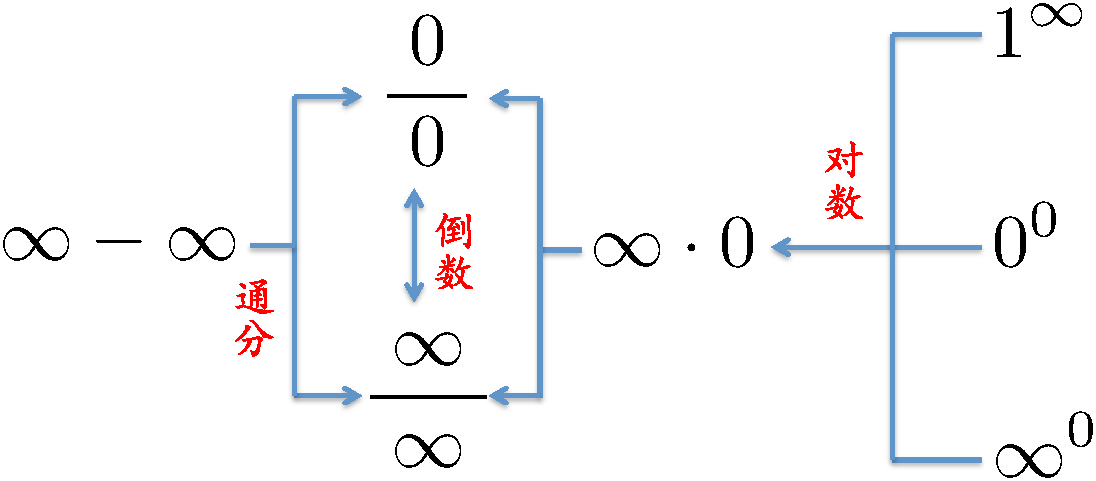
\includegraphics{./images/ch5/lim00.pdf}}
\end{center}

既然不定式极限之间存在这样的转换关系,理论上讲,只要解决了其中的一类问题,则可以将
有关的结果直接推广应用于其他的类型,或者说,总可以将任何一类不定式的问题化为其中的
一个类型(例如$\df{\bm0}{\bm0}$型)的极限来讨论。正因为如此,才有了所谓无穷小
的比较这一说法。

{\bf 定义:}设$\alpha,\beta$均为$x\to\Delta$时的无穷小,且
$\limx{\Delta}\df{\beta}{\alpha}=A$
\begin{enumerate}[(1)]
  \setlength{\itemindent}{1cm}
  \item $A=0$,称$\beta$为$\alpha$当$x\to\Delta$时的{\it 高阶(高级)无穷小},记为:
  \ps{\b 等式中出现无穷小符号$\circ$或$\mathrm{O}$时,等号的含义,准确地
  解释应该是指左侧函数为右侧符号所标识的函数之一!}
  $$\beta=\circ(\alpha)\;\;(x\to\Delta)$$
  \begin{itemize}
    \item {\it 无穷小}可记为:
    $$\beta=\circ(1),\alpha=\circ(1)\;\;(x\to\Delta)$$
  \end{itemize}
  \item $A\ne 0$,称$\beta$为$\alpha$当$x\to\Delta$时的{\it 同阶(同级)无穷小},记为:
  $$\beta=\mathrm{O}(\alpha)\;\;(x\to\Delta)$$
  \item $A=1$,称$\beta$为$\alpha$当$x\to\Delta$时的{\it 等价无穷小},记为:
  $$\beta\sim \alpha\;\;(x\to\Delta)$$
\end{enumerate}

{\bf 注意:}{\it\b 所有的无穷小都必须是和某个$x\to\Delta$相关的,因此讨论
无穷小性质或者对其进行计算、推导时,必须说明是在怎样的$x$变化趋势之中!!!}

\begin{shaded}
	{\bf 高阶无穷小的演算}
	
	对包含有无穷小符号的表达式进行推导,不可避免地会涉及一些化简、合并运算,以下是一些常用
	的化简形式,以$x\to 0$时的无穷小为例:
	\begin{enumerate}[(1)]
  	  \setlength{\itemindent}{1cm}
  	  \item $C\cdot\circ(x^n)=\circ(x^n)\;(C\in\mathbb{R}\mbox{为常数})$
	  \item $x^n=\circ(x^m)\quad (m<n)$ 
	  \item $\circ(x^n)=x^n\cdot\circ(1)$
	  \item $\circ(x^n)\pm\circ(x^n)=\circ(x^n)$
	  \item $x^n\cdot\circ(x^m)=\circ(x^{m+n})$ 
	  \item $\circ(x^n)+\circ(x^m)=\circ(x^n)\;(m\geq n)$  
	  \item $\circ(x^n)\cdot\circ(x^m)=\circ(x^{m+n})$
	\end{enumerate}
	
	要正确理解以上的表达式,必须注意到其中的等号的意义与我们惯常使用的有所不同,其含义
	不是指表达式两边恒等,而应该理解成类似集合运算中的属于关系,例如:$x^n=\circ(x^m)\quad (m<n)$ 
	应该理解为$x_n$是所有$x^m$的高阶无穷小中的一个(属于$\circ(x^m)$所标识的一族函数);
	$x^n\cdot\circ(x^m)=\circ(x^{m+n})$应该理解为,一个$x^m$的高阶无穷小,乘以
	$x^n$,所得函数是$x^{m+n}$的一个高阶无穷小中(属于$\circ(x^{m+n})$所标识的
	一族函数)。事实上,所有包含了高阶无穷小的等式,其中的等号都应该做类似的理解!
	
	在今后的极限计算中,我们可能会用到Taylor展开式,例如:
	\begin{align}
		\limx{0}\df{e^{x^2}-\cos x}{x^2}&=\limx{0}
		\df{1+x^2+\circ(x^2)-1+\df{x^2}2+\circ(x^2)}{x^2}\notag\\
		&=\limx{0}\df{\df32x^2+\circ(x^2)}{x^2}=\df32\notag
	\end{align}
\end{shaded}

% \subsection{(等价)无穷小代换}

不难证明,等价无穷小具有如下的一些性质:
\begin{itemize}
  \setlength{\itemindent}{1cm}
  \item $\beta\sim\alpha\Leftrightarrow\beta=\alpha+\circ(\alpha)$,或者
	$\alpha=\beta+\circ(\beta)$;
  \item {\it 自反性:} $y\sim y$ ;
  \item {\it 对称性:} $y_1\sim y_2\Rightarrow y_2\sim y_1$; 
  \item {\it 传递性:} $y_1\sim y_2,y_2\sim y_3\Rightarrow y_1\sim y_3$。 
\end{itemize}

由它们,进一步可以得到如下关于等价无穷小代换的定理:

{\bf 定理:}设$\alpha\sim \beta\;(x\to\Delta)$,则
$$\limx{\Delta}\alpha\gamma=A
\quad\Leftrightarrow\quad\limx{\Delta}\beta\gamma=A.$$

这个定理意味着,极限“{\it 乘法因子}”中的等价无穷小可相互替代,这对于我们简化极限运算会大有帮助。
例如:当$x\to 0$时,我们有$\sin x\sim x$且$1-\cos x\sim\df12x^2$,故
$$\limx0\df{\sin x^2}{1-\cos x}=\limx0\df{x^2}{\frac{x^2}2}=2.$$

{\bf 问:}如果不是乘法因子,这样的代换还能正确进行吗?

[答]:不能保证结果的正确!例如极限$\limx0\df{\tan x-\sin x}{x^3}$。

如果直接进行代换,由$\tan x\sim x,\sin x\sim x$,可得
$$\limx0\df{\tan x-\sin x}{x^3}=\limx0\df{x-x}{x^3}=0.$$
但是,正确的结果应该是这样的:
$$
	\limx0\df{\tan x-\sin x}{x^3}
	=\limx0\df{\sin x(1-\cos x)}{x^3\cos x}
	=\limx0\df{x\frac{x^2}2}{x^3\cos x}
	=\limx0\df1{2\cos x}=\df12.
$$

{\b 一些常用的等价无穷小:$x\to 0$时,
\begin{enumerate}[(1)]
  \setlength{\itemindent}{1cm}
  \item $x\sim \sin x\sim \tan x$ 
  \item $x \sim\arcsin x\sim\arctan x$ 
  \item $1-\cos x\sim \df 12 x^2$ 
  \item $(1+x)^a-1\sim ax$ 
  \item $\ln(1+x)\sim x$ 
  \item $a^x-1\sim x\ln a\;(a>0)$
\end{enumerate}}

{\bf 例:}计算极限
\begin{enumerate}[(1)]
  \setlength{\itemindent}{1cm}
  \item $\limx{0}\df{\arctan x}{\sin 4x}=\df14$ 
  \item $\limx{0}\df{\ln\cos ax}{\ln\cos bx}=\limx{0}\df{1-\cos ax}{1-\cos
  bx}=\df{a^2}{b^2}$
  \item $\limx{0}\df{\cos x(e^{\sin x}-1)^4}{\sin^2 x(1-\cos x)}=2$ 
  \item $\limx{0}\df{\sin x-\tan x}{x^3}=\limx{0}\df{\cos x-1}{x^2\cos
  x}=-\df12$
\end{enumerate}

{\bf 补充例题:}

{\bf 例:}计算以下极限
\begin{enumerate}[(1)]
  \setlength{\itemindent}{1cm}
  \item $\limx{+\infty}(\sqrt{x^2+x+1}-\sqrt{x^2+x-1})$ 
  \item $\limx{0}\df{\sqrt[3]{1+x}-1}{x}$ 
  \item $\limx{0}\df{\sqrt{1-\cos x^2}}{1-\cos x}$ 
  \item $\limx{0}\df{1-\cos x\cos 2x}{1-\cos x}$
  \item $\limx{\pi /4}(\tan x)^{\tan 2x}$ 
  \item $\limx{0}\left(2e^{\frac{x}{x+1}}-1\right)^{\frac{x^2+1}{x}}$ 
  \item $\limx{+\infty}\left(\sqrt{x^2+x}-\sqrt[3]{x^3+x^2}\right)$ 
  \item $\limx{+\infty}\left(\df{x^2-1}{x^2+1}\right)^{x^2}$
  \item $\limx{0}\left(\df{a^x+b^x+c^x}{3}\right)^{1/x}\,(a,b,c>0)$ 
  \item $\limx{0}\left(\df{a^{x+1}+b^{x+1}+c^{x+1}}{a+b+c}\right)^{1/x}
  \,(a,b,c>0)$ 
  \item $\limx{0}\df{\tan(\tan x)-\sin(\sin x)}{\tan x-\sin x}$
  \item $\limx0\df{\sqrt[n]{1+\sin x}-1}{\tan x}$
  \item $\limx0(x+e^x)^{\frac1x}$
  \item $\limx0\left(\df{e^x+xe^x}{e^x-1}-\df1x\right)$
  \item $\limn\ln\left(\df{n-2na+1}{n(1-2a)}\right)^n\quad(a\ne1/2)$
  \item $\limx0\df{[\sin-\sin(\sin x)]\sin x}{x^4}$
  \item $\limx0\df{e^{\tan x}-e^{\sin x}}{x\sin^2x}$
  \item $\limx0\df{\sqrt{1+\tan x}-\sqrt{1+\sin x}}{x(1-\cos x)}$
  \item $\limn\left(n\tan\df1n\right)^{n^2}$
  \item $\limx0\df{\sin x+x^2\sin\df1x}{(1+\cos x)\ln(1+x)}$
  \item $\limx0\left[\df
  ax-\left(\df1{x^2}-a^2\right)\ln(1+ax)\right]$\quad($a\ne 0$)
  \item $\limx{\infty}\df{(x+a)^{x+a}(x+b)^{x+b}}{(x+a+b)^{2x+a+b}}$
  \item $\limx{0^+}\df{x^x-(\sin x)^x}{x^2\ln(1+x)}$
  \item $\limx0\df{\cos x-e^{-\frac{x^2}2}}{x^2[x+\ln(1-x)]}$
  \item $\limx{+\infty}\left(x+e^x\right)^{\frac1x}$
  \item $\limx{+\infty}\left(x+\sqrt{1+x^2}\right)^{\frac1x}$
  \item $\limx0\df{\sin x-x\cos x}{\sin^3x}$
  \item $\limx{+\infty}\df{e^x}{\left(1+\df1x\right)^{x^2}}$
  \item $\limx0\df1{x^3}\left[\left(\df{2+\cos x}3\right)^x-1\right]$
  \item $\limx0\df{\ln(\sin^2x+e^x)-x}{\ln(x^2+e^{2x})-2x}$
  \item $\limx1\df{x-x^x}{1-x+\ln x}$
  \item $\limx0\df{1-\cos x\sqrt{\cos2x}}{x^2}$
  \item $\limx{0^+}\df{\ln(1+e^{\frac2x})}{\ln(1+e^{\frac1x})}$
  \item $\limx{+\infty}\df{e^x-e^{-x}}{e^x+e^{-x}}$
  \item $\limx0\left(\df1n\sum\limits_{k=1}^na_k^x\right)^{\frac1x}
  \quad (a_k>0,k=1,2,\ldots,n)$
  \item $\limn n^2\left(\arctan\df an-\arctan\df a{n+1}\right)\quad (a>0)$
  \item $\limx0\df{(1+x)^{\frac1x}-(1+2x)^{\frac1{2x}}}{\sin x}$
  \item $\limn\left[\left(n^3-n^2+\df n2\right)e^{\frac1n}-\sqrt{1+n^6}\right]$
\end{enumerate}

{\bf 例:}若$x\to 0$时,$\ln\left(\cos\df{2x}3\right)\sim Ax^k$,则
$A=$\underline{$-\df29$},$k=$\underline{$2$}

{\bf 例:}设$\limx0\df{\ln\left(1+\df{f(x)}{\sin x}\right)}{a^x-1}=A\;(a\ne 1)$,求
$\limx0\df{f(x)}{x^2}$

{\bf 例:}设$\limn\df{n^a}{n^b-(n-1)^b}=10$,则$a=\underline{-9/10},
b=\underline{1/10}$

[提示]:
$\limn\df{n^a}{n^b-(n-1)^b}=10=\limn\df{n^{a-b}}{1-\left(1-\df1n\right)^b}
=\limn\df{n^{a-b+1}}b,$
由此可知,显然$b\ne 0$,且只有当$a-b+1=0$时,极限为为零有限值。

数列掌握和应用等价无穷小代换,能够使我们在计算极限值时获得很大的便利,但是必须指出的是,
到目前为止,还存在相当多的极限问题是我们无法求解的,例如:
$$\limx0\df{x-\sin x}{x^3},
\quad\limx0\df{e^x-\cos x}x,$$
这些题目需要我们在后续章节中学习的L'Hospital法则和Taylor公式等新的工具。
特别值得一提的是,学习完Taylor公式后,我们将会对无穷小的认识有一个大大深入的理解和认识。

\section{函数的连续性}

\subsection{函数连续的概念}

{\bf 函数$f(x)$在$x_0$连续},也即:
$$\b\limx{x_0}f(x)=f(x_0).$$
如果记$\Delta y=f(x_0+\Delta x)-f(x_0)$,则函数连续也可以等价地表示为:
$$\b\lim\limits_{\Delta x\to 0}\Delta y=0.$$

直观地理解,就是在$x_0$左右两侧的函数值都趋于相同的极限(左右极限相等),
且极限值恰好是这一点处的函数值。因此,函数连续也等价于
\begin{itemize}
  \setlength{\itemindent}{1cm}
  \item $f(x)$在$x_0$有定义; 
  \item $\limx{x_0}f(x)$存在; 
  \item $f(x_0)=f(x_0+0)=f(x_0-0)$。
\end{itemize}
以上三者都是函数连续的必要条件。

从代数运算的意义上,函数连续等价于该函数的运算可以和极限运算交换次序,因为
连续的定义事实上也可以写为:
$$\b\limx{x_0}f(x)=f(\limx{x_0}x).$$

{\bf 注:}必要时,可以只考虑函数在某点一侧的连续性,即所谓{\it 左(右)连续}。

{\bf 例:}证明:$f(x)=xD(x)$只在$x=0$处连续。
\ps{在现实世界里,没有只在一个点连续的曲线,这是数学概念和直观现实存在差异的一个很好的例证}

[提示]:先证明$xD(x)$仅在$x=0$处极限存在。

{\bf 例:}\ps{KD教材3.4.1节-例3}
设$f(x)$在$(-\infty,+\infty)$上有定义,
且对任意$x,y\in (-\infty,+\infty)$,有
$$f(x+y)=f(x)+f(y),$$
则$f(x)$在$(-\infty,+\infty)$上连续,当且仅当$f(x)$在$x=0$连续。

% \begin{center}
% 	\resizebox{!}{4cm}{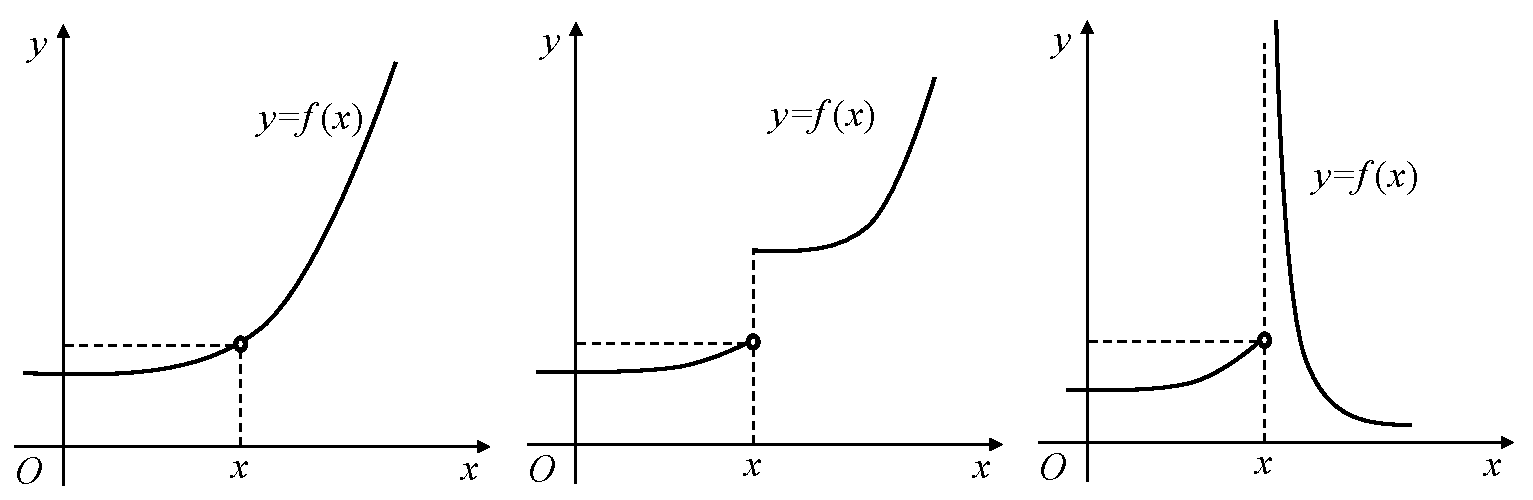
\includegraphics{./images/ch3/notCont.pdf}}
% \end{center}

\subsection{函数的间断点}

{\b 间断点}即不连续点,根据前述函数连续的必要条件,可以对间断点作出如下的分类:

设$x_0$是$f(x)$的间断点(不连续点),对其分类定义如下:
\ps{此处的第一类、第二类间断点的分类,沿用了KD教材的定义}
\begin{enumerate}[(1)]
  \setlength{\itemindent}{1cm}
  \item {\it 第一类间断点:}$f(x_0+0),f(x_0-0)$均存在
  \begin{itemize}
    \item {\it 跳跃间断点:}$f(x_0+0)\ne f(x_0-0)$,例:$y=[x]$当$x$为整数时
    \begin{center}
		\resizebox{!}{4cm}{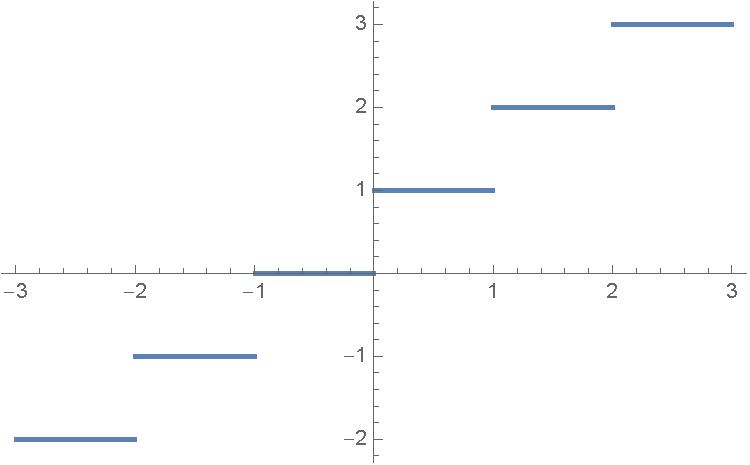
\includegraphics{./images/ch3/roundx.pdf}}
 	\end{center}
    \item {\it 可去间断点:}$f(x_0)$无定义,或
    $$f(x_0)\ne f(x_0+0)=f(x_0-0)$$
    例:$y=\df{\sin x}x$在$x=0$处
    \begin{center}
		\resizebox{!}{4cm}{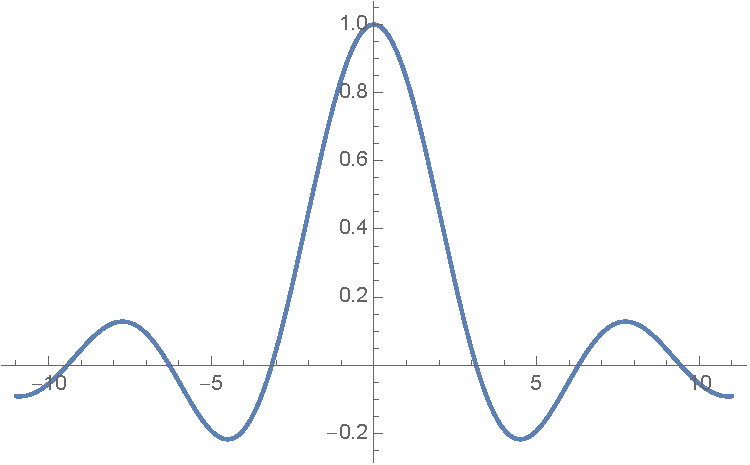
\includegraphics{./images/ch3/sinxox.pdf}}
 	\end{center}
  \end{itemize}
  \item {\it 第二类间断点:}$f(x_0+0),f(x_0-0)$不同时存在
  \begin{itemize}
    \item {\it 无穷间断点:}某个单侧极限趋于无穷,例:$y=\tan x$和$y=\sec x$在$x=k\pi+\df{\pi}2$处
     \begin{center}
		\resizebox{!}{4cm}{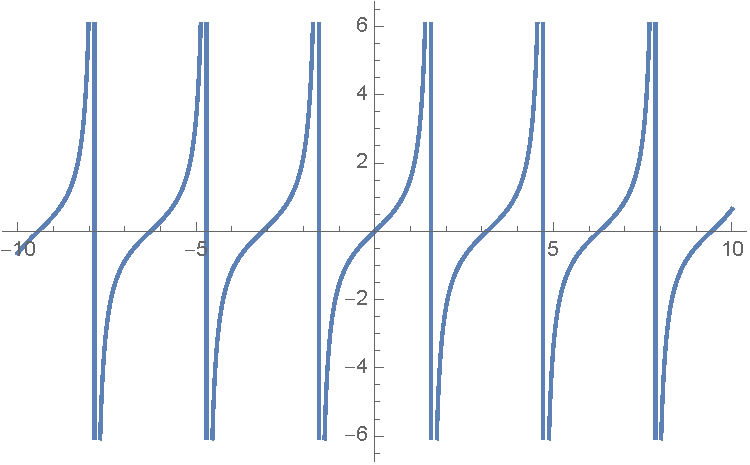
\includegraphics{./images/ch3/tanx.pdf}}
		\resizebox{!}{4cm}{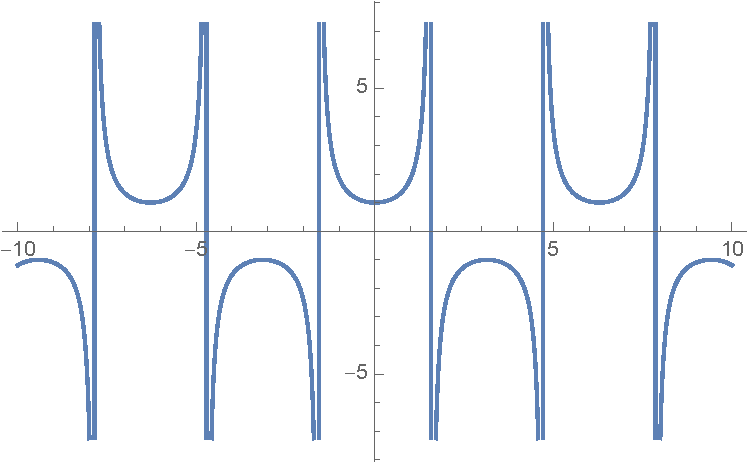
\includegraphics{./images/ch3/secx.pdf}}
 	\end{center}
    \item {\it 振荡间断点:}某个单侧极限不存在,且非无穷,例:$y=\sin\df1x$在$x=0$处
    \begin{center}
		\resizebox{!}{5cm}{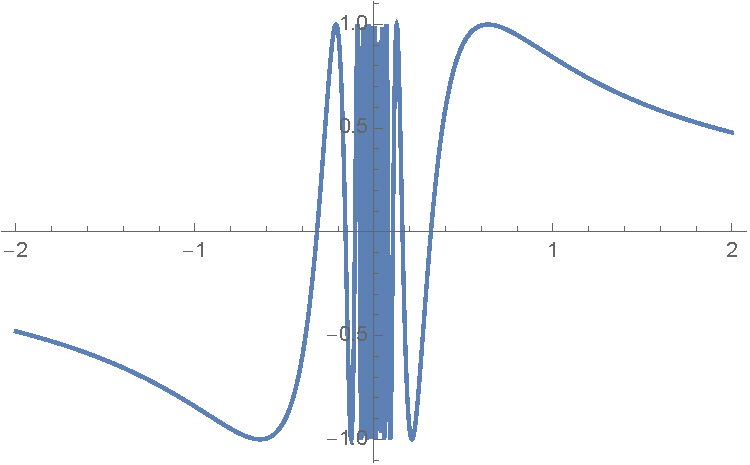
\includegraphics{./images/ch3/sin1ox.pdf}}
 	\end{center}
  \end{itemize}
\end{enumerate}

{\bf 例:}指出以下函数的间断点,判断其类型
\begin{enumerate}[(1)]
  \setlength{\itemindent}{1cm}
  \item $y=\df{x^2-1}{x-1}$\quad{\it 可去}
  \item $y=\df{x^2+1}{x-1}$\quad{\it 无穷}
  \item $y=D(x)$\quad{\it 振荡}
\end{enumerate}

\subsection{连续函数的运算与初等函数的连续性}

\begin{enumerate}[(1)]
  \setlength{\itemindent}{1cm}
  \item {\it 四则运算:} 四则运算仍保持函数的连续性; 
  \item {\it 复合函数:} 连续函数的函数运算可以和极限运算交换次序; 
  \item {\it 反函数:} 连续函数的反函数也连续 ;
  \item {\it 初等函数:} 初等函数在其{\it 定义区间}内连续;
\end{enumerate}

{\bf 注:}以上的定义区间是指函数定义域内的一个开区间,例如:$y=\df1x$在定义域内整体
是不连续的,但在定义域内的任意一个区间内都连续。

\subsection{闭区间上连续函数的性质}

以下我们引入记号$f(x)\in C(I)$,表示函数$f(x)$在区间$I$上连续。例如:
{\b$f(x)\in C[a,b]$表示函数$f(x)$在闭区间$[a,b]$上连续}。

闭区间上的连续函数有一些“有趣”的性质,这些性质在很大程度上是符合我们对
连续这一概念的直观印象的。

\subsubsection{有界性与最值存在性}

{\bf 最值定理:}$f(x)\in C[a,b]$,则$f(x)$在$[a,b]$上可取到最大和最小值。
{\it 也即,存在$\xi,\eta\in[a,b]$,是对任意$x\in[a,b]$,总有$f(\xi)
\leq f(x)\leq f(\eta)$}

此定理掌握结论即可,无须了解证明。下面的推论是显然的

{\bf 有界性:}$f(x)\in C[a,b]$,则$f(x)$在$[a,b]$上有界。
\ps{提醒注意一点:在闭区间上,连续可以推出有界,但反之不然,请自行思考反例}

利用这一性质,可以证明类似下面的结论:

{\bf 例:}设$f(x)\in C[a,+\infty)$,且$\limx{+\infty}f(x)$存在,
证明:$f(x)$在$[a,+\infty)$上有界。

[提示]:首先利用函数极限的有界性证明,存在$M_1$和$X$,对任意$x>X$,有$|f(x)|<M_1$。
然后,利用连续函数在闭区间上的有界性,说明存在$M_2$,对任意$x\in[a,X]$,有$|f(x)|<M_2$。
综合即证。

{\bf 例:}设$f(x)\in C(\mathrm{R})$,且$f(\infty)$存在,则$f(x)$在$\mathrm{R}$
上有界。

\subsubsection{介值定理和零点存在定理}

{\bf 介值定理:}设$f(x)\in C[a,b]$,$M,m$分别为$f(x)$在$[a,b]$上的最大和最小值,
则对任意$\gamma\in[m,M]$,存在\ps{\b “存在”与“至少存在”意义是完全一致的!}
$\xi\in[a,b]$,使得$f(\xi)=\gamma$。

定理证明不需要掌握,略过。该定理最常用的是如下的推论:

{\bf 零值存在定理:}设$f(x)\in C[a,b]$,且$f(a)f(b)<0$,则$f(x)$在$[a,b]$上必有零点。

和前述关于有界性的讨论类似,零点存在定理也可以进一步作如下的推广:
\begin{enumerate}[(1)]
  \setlength{\itemindent}{1cm}
  \item {\b 设$f(x)\in C(a,b)$,且$f(a+0)\cdot f(b-0)<0$,则$f(x)$在$(a,b)$内有零点。} 
  \item {\b 设$f(x)\in C(-\infty,+\infty)$,且$f(-\infty)\cdot f(+\infty)<0$,
  则$f(x)$在$(-\infty,+\infty)$内有零点。}
\end{enumerate}

[提示]:利用极限的保号性证明。

{\bf 补充例题:}

{\bf 例:}设$a_0\ne 0$,证明:以下方程至少有一个实根\ps{\b 奇数次多项式方程至少有一个实根!}
$$a_0x^{2n+1}+a_1x^{2n}+\ldots+a_{2n}x+a_{2n+1}=0.$$

[提示]:$\limx{\infty}\df{f(x)}{x^{2n+1}}=a_0$,利用极限保号性说明
$f(x)$当$x$充分大(小)时,分别有取正和取负的值。

{\bf 例:}已知$f(x)\in C[0,3]$,且$f(0)=f(3)$,证明:至少存在
一个$\xi\in[0,2]$,使得$f(\xi+1)=f(\xi)$

[证]:设$F(x)=f(x+1)-f(x)$,显然$F(x)\in C[0,2]$。

注意到若$f(0)=f(1)$或$f(1)=f(2)$或$f(2)=f(3)$,结论显然成立。故以下设$f(0)\ne f(1),
f(1)\ne f(2),f(2)\ne f(3)$。

不妨设$f(1)>f(0)$,则$F(0)>0$。此时,若$f(2)<f(1)$,则$F(1)<0$,
由连续函数的介值定理可知必有$\xi\in[0,1]$,使得$F(\xi)=0$。
又若$f(2)>f(1)$,则$F(1)>0$,
$$F(2)=f(3)-f(2)=f(0)-f(2)<f(1)-f(2)=-F(1)<0,$$
同样由连续函数的介值定理可知必有$\xi\in[1,2]$,
使得$F(\xi)=0$。

综上,必有$\xi\in[0,2]$,使得$F(\xi)=0$,也即$f(\xi+1)=f(\xi)$。\hfill $\Box$

{\bf 例:}设$G$是第一象限内的一个有界区域(其边界为连续的简单闭曲线),$ABCD$表示
它的一个外接矩形。矩形的一条边与$x$轴的夹角记为$\theta$,如果对于任意$\theta\in
[0,\pi/2]$,$G$总可以被某个外接矩形所围,证明:至少存在某个$\theta_0\in[0,\pi/2]$,
使得与之对应的外接矩形恰好为正方形。({\it 推论:任一平面有界区域都可以内接于某个正方形})

\begin{center}
	\resizebox{!}{6cm}{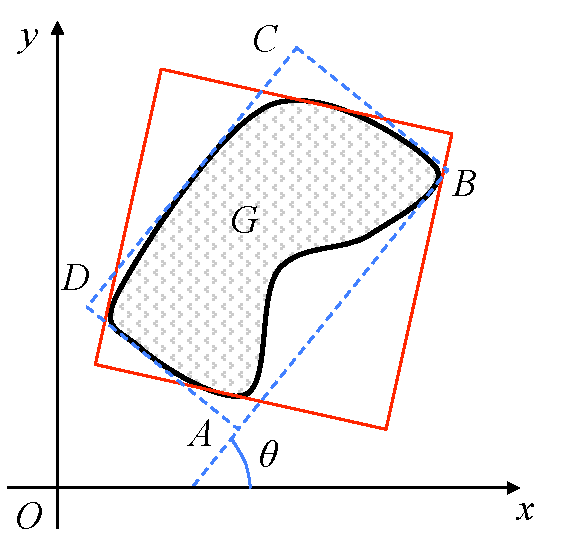
\includegraphics{./images/ch3/sqOut.pdf}}
\end{center}

[提示]:记$l_1(\theta),l_2(\theta)$分别为$AB$和$BC$的长度,显然
$$l_1(0)=l_2(\pi/2),\quad l_2(0)=l_1(\pi/2).$$
令$f(\theta)=l_1(\theta)-l_2(\theta)$,由介值定理可以证明$f(\theta)$存在零点。

{\bf 例:}证明:给定任意平面有界区域,以及一个向量,一定存在一条与该向量平行的直线
平分该区域。

{\bf 例:}证明:给定任意平面有界区域,一定存在两条相互垂直的直线,将其四等分。

[提示]:设其中一条直线的极角为$\theta$,则另一条的为$\theta+\pi/2$。
分别记两条直线为$l_{\theta}$和$l_{\theta+\pi/2}$,显然可以使得二者都平分给定区域。
设此时四个区域的面积按顺时针方向依次为$S_1,S_2,S_3,S_4$,且由平分可满足
$$A_1+A_2=A_3+A_4,\quad A_1+A_4=A2+A_3,$$

\begin{center}
	\resizebox{!}{6cm}{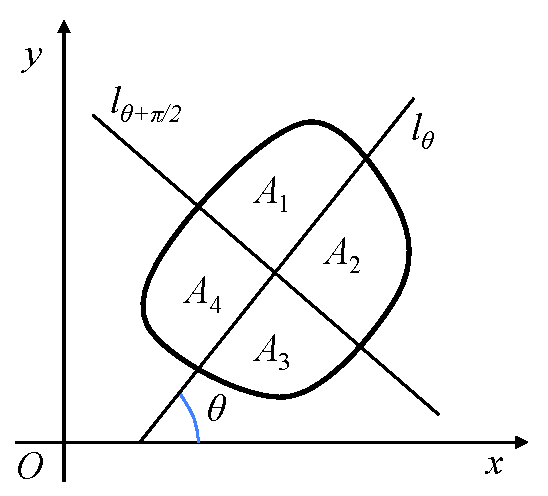
\includegraphics{./images/ch3/4cut.pdf}}
\end{center}

由此可得
$$A_1=A_3,\quad A_2=A_4.$$
进而,只需适当取$\theta$,使得$A_1=A_2$即可。

记$f(\theta)=A_1(\theta)-A_2(\theta)$,不妨设$f(0)>0$,从而
$$f(\pi/2)=A_1(\pi/2)-A_2(\pi/2)=A_4(0)-A_1(0)=A_2(0)-A_1(0)=-f(0)<0,$$
由介值定理,即证。

{\bf 例:}任意金属圆环上,总存在相对的两点温度相同。
({\it 圆环可以看成赤道,温度即为两点的气温})

[提示]:默认假设温度总是连续分布的。

{\bf 思考:}构造更多类似的例题,用介值定理证明某种状态的存在性。

% \subsubsection{一致连续性}
% 
% 略

\section*{小结}
\addcontentsline{toc}{section}{小结}

数列极限是我们研究和讨论更一般的函数极限的基础,因为其典型性和相对简单直观的性质,成为了
我们进入微积分的起始点。

本章的一个难点是{\it 数列极限的“$\e-N$”定义},能够准确叙述定义,并使用其来证明一些极限
对于很多同学来说需要付出巨大的能力。通过这部分的学习,能使大家对什么是严谨的数学和逻辑推理,
怎样作到数学表达的严密和精确有一个初步的体验。

就目前来看,用定义证明数列极限从未作为各级高数考试的重点,这可以说是非常幸运的。
而本章真正的重点,毫无疑问,是数列极限的判敛和计算。我们介绍了一些典型的方法
和常用技巧,包括:{\it 子数列的性质、夹逼定理、单调有界原理、递推数列的判敛、
Stolz定理等}。对所有这些方法的理解和纯熟掌握本章学习的目标之一。

函数极限与数列极限最明显的不同,就是所考虑的自变量变化过程,从单一的趋于正无穷扩展到了
趋于无穷和趋于有限值两大类,共六种不同的过程。

在学习函数极限的概念,或者说“$\e-X$”(“$\e-\delta$”)定义时,一定要注意和数列极限
的“$\e-N$”定义进行类比,严格来说,在所有这些不同极限的定义中,有所变化的只是所趋近的目标
(无穷或有限值)的邻域概念,定义的结构和内涵都是完全一样的,即:{\it 只要自变量充分靠近
趋近的目标,则函数值也会充分靠近某个稳定的值。}

正因文定义上的相似,所以在基本的性质上,函数极限和数列极限也没有本质的不同。需要注意
的仅仅是有些性质在表述上的变化,例如{\it 函数极限的有界性}和数列极限的有界性在表述上就存在
明显的差别,能够正确表述函数极限的有界性,是本章学习的第一个有挑战的知识点。

和数列极限一样,本章学习的重点是函数极限的判敛和计算问题,特别是后者。我们所学习的{\it 两个
重要极限和众多由它们衍生的常用极限},是我们今后计算很多极限的基础。在此需要提醒同学们的是,
拿到一个极限问题,首先要判断其基本的形态(例如:“$0/0$”,“$1^{\infty}$”),然后
根据其形态上的特点选择运算的方向(或者说变换的目标),最终将其化为一些我们常见或者说
基本的极限。这一点,常常被很多同学所忽视。

无穷小的概念是微积分真正成为一门新学科,在数学理论中确立其独特地位的源头。Newton最早
有意识地使用了无穷小的概念,并利用其种种性质达到简化计算和推理的目的,但无穷小的有关理论是在
其诞生后近百年后才真正稳固的。也正因为如此,无穷小也是本章学习的难点和重点。所谓的难点,
主要体现在对无穷小的“运算”方法(例如:$\circ(x^2)+\circ(x)=\circ(x)$)的理解,以及
何时可以在有关的计算(不仅仅是极限问题)中准确地将其忽略不计。至于其重要性可以说是不言而喻
的,{\it 无穷小代换}的思想对于我们计算各种不定式的极限给出了崭新的思路和表述方法,极大提高了
极限计算的效率。在本章之外,无穷小的故事还会继续。

函数的连续性概念源于生活的直觉,但并不等同于直觉,事实上,在现实中就没有“在某一点连续”
的直觉对应。{\it 函数连续的本质是,函数运算和极限运算可以交换次序},换句话说,对于在某点连续的
函数而言,计算其在该点的极限和计算其函数值没有什么不同。

{\it 有界闭区间上连续函数的性质}是本章最富有趣味也是颇具挑战性的问题,特别是和我们后续
学习中的中值定理相结合,将展示给大家极为丰富和多样化的挑战性问题,并成为本门课程的又一个
标志性的难点。

\newpage

\section*{课后作业}
\addcontentsline{toc}{section}{课后作业}
% {\bf 【必作题】}
{\b\it 说明:作业必须写明题目所在章节、页码、题号;如非特别说明,
所有题目必须抄题;两道题之间空一行;未作或作错的题目讲评后务必及时订正。}

\begin{itemize}
  \item 注册加入课程网站:https://www.trustie.net/courses/1259,邀请码:YRKWF
  \item 注册中学大学MOOC账号:http://www.icourses.cn/imooc/,将用户名告知课代表
  统一登记
  
  {\b\it 下面的题目请写在活页纸上,不用抄题:}
  \item 写一篇短文,内容及要求如下
  \begin{enumerate}[(1)]
    \item 你的个人介绍,请务必包含如下信息:姓名、性别、年龄、籍贯、中学母校的名字、
    你的高考总成绩(以及当地的满分)、你的高考数学成绩(以及当地的满分);
    \item 你的兴趣爱好、特长,或者说,你觉得自己有什么与众不同之处;
    \item 你学习数学的体会,例如:喜欢,不喜欢?喜欢什么样的数学,不喜欢什么样的数学?
    有什么好的学习方法?有什么自己觉得成功的经验,或者有趣的经历(最好与数学有关)?
    \item 你期待中的大学课堂是怎样的?怎么的教与学会对你更有帮助?对老师有什么期待、要求,
    或者建议?
    \item 请至少推荐一本(部、套)你喜欢的书、电影或者其他任何可以通过公共渠道获取到的资料
    (例如:网站、软件、APP、\ldots),说说推荐的理由;
    \item 其他任何你认为值得(可以)与我交流的东西,比如你想问我什么问题;
    \item 除第一条必须包含外,其余内容可自由取舍。
    \item 篇幅:不少于半页,不多于两页(一张纸的正反面)。
  \end{enumerate}
  {\b\it 以下的题目写在作业本上,作业本第一页背面上贴上一张个人的照片,标注专业和籍贯}
  \item 习题1-2:5(3,4),7,8
  \item 习题1-3:5(3),6(2),7,8
  \item 习题1-4:7,8
  \item 习题1-5:3
  \item 习题1-6:4(2,3,5)
  \item 习题1-7:4(2),5(3,4)
  \item 习题1-8:4
  \item 习题1-9:2,3(3,5,6),4
  \item 习题1-10:1,5,7
  \item 总习题一:14
\end{itemize}

% \bigskip
% 
% \hrule
% 
% \bigskip
% \bigskip
% 
% {\bf 【思考题】}\ps{\b 思考题主要作为课后的辅助阅读,欢迎课间找我讨论,不必写在作业纸上}
% 
% \begin{itemize}
% %   \item 习题1.1:(C)应用题
%   \item 习题1.2:13,17,22,23
%   \item 习题1.3:6,7,9
%   \item 习题5.2:3
%   \item 阅读:李开复,《给未来的你》
% \end{itemize}